\documentclass[11pt,a4paper,dvipsnames,twosided]{article}
\usepackage[deliverable]{IOHKCoverPage}

% data for Deliverable header -- added by KH from an EU H2020 project template
\DeliverableNumber{SL-D5}
\DeliverableTitle{A Formal Specification of the Cardano Ledger}{Formal Cardano Ledger Spec.}
\DeliverableResponsible{Formal Methods Team}
\EditorName{Jared Corduan, \IOHK}
\Authors{Jared Corduan \quad \texttt{<jared.corduan@iohk.io>}
   \\[1em]
   Polina Vinogradova \quad \texttt{<polina.vinogradova@iohk.io>}
   \\[1em]
   Matthias G\"udemann \quad \texttt{<matthias.gudemann@iohk.io>}
}
\DueDate{15$^{\textrm{th}}$ October 2019}
\SubmissionDate{8th October 2019}{2019/10/08}
\LeaderName{Philipp Kant, \IOHK}
\InstitutionAddress{\IOHK}
\Version{1.0}
\Project{Shelley Ledger}
\DisseminationPU

\usepackage[margin=2.5cm]{geometry}
\usepackage{lscape}
\usepackage{iohk}
\usepackage{microtype}
\usepackage{mathpazo} % nice fonts
\usepackage{amsmath}
\usepackage{amssymb}
\usepackage{amsthm}
\usepackage{latexsym}
\usepackage{mathtools}
\usepackage{stmaryrd}
\usepackage{extarrows}
\usepackage{slashed}
\usepackage[unicode=true,pdftex,pdfa,colorlinks=true]{hyperref}
\usepackage{xcolor}
\usepackage[capitalise,noabbrev,nameinlink]{cleveref}
\usepackage{float}
\floatstyle{boxed}
\restylefloat{figure}
\usepackage{tikz}
\usepackage{booktabs}
\usepackage{enumerate}
\usepackage{listings}
%%
%% Package `semantic` can be used for writing inference rules.
%%
\usepackage{semantic}
%% Setup for the semantic package
\setpremisesspace{20pt}

\usepackage{tocloft}
\addtolength{\cftsubsecnumwidth}{5pt}

%%
%% Types
%%
\newcommand{\Nothing}{\ensuremath{\Diamond}}
\newcommand{\N}{\ensuremath{\mathbb{N}}}
\newcommand{\Bool}{\type{Bool}}
\newcommand{\Npos}{\ensuremath{\mathbb{N}^{>0}}}
\newcommand{\Z}{\ensuremath{\mathbb{Z}}}
\newcommand{\Q}{\ensuremath{\mathbb{Q}}}
\newcommand{\R}{\ensuremath{\mathbb{R}}}
\newcommand{\Rnn}{\ensuremath{\mathbb{R}^{\geq 0}}}
\newcommand{\Tx}{\type{Tx}}
\newcommand{\TxBody}{\type{TxBody}}
\newcommand{\TxWitness}{\type{TxWitness}}
\newcommand{\Ix}{\type{Ix}}
\newcommand{\TxId}{\type{TxId}}
\newcommand{\Addr}{\type{Addr}}
\newcommand{\UTxO}{\type{UTxO}}
\newcommand{\Wdrl}{\type{Wdrl}}
\newcommand{\Coin}{\type{Coin}}
\newcommand{\PParams}{\type{PParams}}
\newcommand{\PParamsUpdate}{\type{PParamsUpdate}}
\newcommand{\ProposedPPUpdates}{\type{ProposedPPUpdates}}
\newcommand{\Slot}{\type{Slot}}
\newcommand{\StabilityWindow}{\ensuremath{\mathsf{StabilityWindow}}}
\newcommand{\RandomnessStabilisationWindow}{\ensuremath{\mathsf{RandomnessStabilisationWindow}}}
\newcommand{\SlotsPerEpoch}{\mathsf{SlotsPerEpoch}}
\newcommand{\SlotsPerKESPeriod}{\mathsf{SlotsPerKESPeriod}}
\newcommand{\MaxMajorPV}{\mathsf{MaxMajorPV}}
\newcommand{\ActiveSlotCoeff}{\mathsf{ActiveSlotCoeff}}
\newcommand{\Network}{\mathsf{Network}}
\newcommand{\NetworkId}{\mathsf{NetworkId}}
\newcommand{\BlockNo}{\type{BlockNo}}
\newcommand{\MaxKESEvo}{\ensuremath{\mathsf{MaxKESEvo}}}
\newcommand{\Quorum}{\ensuremath{\mathsf{Quorum}}}
\newcommand{\MaxLovelaceSupply}{\ensuremath{\mathsf{MaxLovelaceSupply}}}
\newcommand{\Duration}{\type{Duration}}
\newcommand{\StakePools}{\type{StakePools}}
\newcommand{\Seed}{\type{Seed}}
\newcommand{\seedOp}{\star}
\newcommand{\Ppm}{\type{Ppm}}
\newcommand{\ProtVer}{\ensuremath{\type{ProtVer}}}
\newcommand{\Metadatum}{\ensuremath{\type{Metadatum}}}
\newcommand{\Metadata}{\ensuremath{\type{Metadata}}}
\newcommand{\MetadataHash}{\ensuremath{\type{MetadataHash}}}
\newcommand{\Update}{\type{Update}}
\newcommand{\GenesisDelegation}{\type{GenesisDelegation}}
\newcommand{\FutGenesisDelegation}{\type{FutGenesisDelegation}}

\newcommand{\DCert}{\type{DCert}}
\newcommand{\DCertRegKey}{\type{DCert_{regkey}}}
\newcommand{\DCertDeRegKey}{\type{DCert_{deregkey}}}
\newcommand{\DCertDeleg}{\type{DCert_{delegate}}}
\newcommand{\DCertRegPool}{\type{DCert_{regpool}}}
\newcommand{\DCertRetirePool}{\type{DCert_{retirepool}}}
\newcommand{\DCertGen}{\type{DCert_{genesis}}}
\newcommand{\DCertMir}{\type{DCert_{mir}}}
\newcommand{\PoolParam}{\type{PoolParam}}
\newcommand{\PoolMD}{\type{PoolMD}}
\newcommand{\MIRPot}{\type{MIRPot}}
\newcommand{\InstantaneousRewards}{\type{InstantaneousRewards}}
\newcommand{\ReservesMIR}{\type{ReservesMIR}}
\newcommand{\TreasuryMIR}{\type{TreasuryMIR}}
\newcommand{\URL}{\type{Url}}
\newcommand{\UTxOState}{\ensuremath{\type{UTxOState}}}
\newcommand{\ledgerState}{\ensuremath{\type{ledgerState}}}

\newcommand{\AddrRWD}{\type{Addr_{rwd}}}
\newcommand{\AddrB}{\type{Addr_{base}}}
\newcommand{\AddrP}{\type{Addr_{ptr}}}
\newcommand{\AddrE}{\type{Addr_{enterprise}}}
\newcommand{\AddrBS}{\type{Addr_{bootstrap}}}
\newcommand{\Ptr}{\type{Ptr}}
\newcommand{\DState}{\type{DState}}
\newcommand{\DWEnv}{\type{DWEnv}}
\newcommand{\DPSEnv}{\type{DPSEnv}}
\newcommand{\DPEnv}{\type{DPEnv}}
\newcommand{\DEnv}{\type{DEnv}}
\newcommand{\PEnv}{\type{PEnv}}
\newcommand{\DPState}{\type{DPState}}
\newcommand{\PState}{\type{PState}}
\newcommand{\DCertBody}{\type{DCertBody}}
\newcommand{\TData}{\type{TData}}
\newcommand{\DPoolReap}{\ensuremath{\type{poolreap}}}
\newcommand{\UPIState}{\type{UPIState}}
\newcommand{\UpdatePayload}{\type{UpdatePayload}}

% multi-signature
\newcommand{\StakeCredential}{\type{Credential}_{stake}}

\newcommand{\txwitsVKey}[1]{\fun{txwitsVKey}~\var{#1}}
\newcommand{\txwitsScript}[1]{\fun{txwitsScript}~\var{#1}}

\newcommand{\AddrVKey}{\type{Addr^{vkey}}}
\newcommand{\AddrRWDVKey}{\type{Addr_{rwd}^{vkey}}}
\newcommand{\AddrRWDScr}{\type{Addr_{rwd}^{script}}}
\newcommand{\AddrVKeyB}{\type{Addr^{vkey}_{base}}}
\newcommand{\AddrVKeyP}{\type{Addr^{vkey}_{ptr}}}
\newcommand{\AddrVKeyE}{\type{Addr^{vkey}_{enterprise}}}
\newcommand{\AddrVKeyBS}{\type{Addr^{vkey}_{bootstrap}}}
\newcommand{\AddrScr}{\type{Addr^{script}}}
\newcommand{\AddrScrBase}{\type{Addr_{base}^{script}}}
\newcommand{\AddrScrEnterprise}{\type{Addr_{enterprise}^{script}}}
\newcommand{\AddrScrPtr}{\type{Addr_{ptr}^{script}}}
\newcommand{\HashScr}{\type{ScriptHash}}
\newcommand{\Script}{\type{Script}}
\newcommand{\MSig}{\type{MSig}}
\newcommand{\Credential}{\type{Credential}}

%% Adding witnesses
\newcommand{\TxIn}{\type{TxIn}}
\newcommand{\TxOut}{\type{TxOut}}
\newcommand{\VKey}{\type{VKey}}
\newcommand{\VKeyEv}{\type{VKey_{ev}}}
\newcommand{\VKeyGen}{\type{VKey_G}}
\newcommand{\SKey}{\type{SKey}}
\newcommand{\SKeyEv}{\type{SKey_{ev}}}
\newcommand{\KeyHash}{\type{KeyHash}}
\newcommand{\KeyHashGen}{\type{KeyHash_G}}
\newcommand{\KeyPair}{\type{KeyPair}}
\newcommand{\KeyPairEv}{\type{KeyPair_{ev}}}
\newcommand{\Sig}{\type{Sig}}
\newcommand{\Data}{\type{Data}}
\newcommand{\Ser}{\type{Ser}}
%% Adding delegation
\newcommand{\Epoch}{\type{Epoch}}
\newcommand{\KESPeriod}{\type{KESPeriod}}
%% Blockchain
\newcommand{\Acnt}{\type{Acnt}}
\newcommand{\Gkeys}{\var{G_{keys}}}
\newcommand{\Block}{\type{Block}}
\newcommand{\SlotId}{\type{SlotId}}
\newcommand{\PPUpdateState}{\type{PPUpdateState}}
\newcommand{\PPUpdateEnv}{\type{PPUpdateEnv}}
\newcommand{\UTxOEnv}{\type{UTxOEnv}}
\newcommand{\CEEnv}{\type{CEEnv}}
\newcommand{\CEState}{\type{CEState}}
\newcommand{\BDEnv}{\type{BDEnv}}
\newcommand{\BDState}{\type{BDState}}
\newcommand{\LEnv}{\type{LEnv}}
\newcommand{\LState}{\type{LState}}

\newcommand{\Proof}{\type{Proof}}
\newcommand{\Seedl}{\mathsf{Seed}_\ell}
\newcommand{\Seede}{\mathsf{Seed}_\eta}
\newcommand{\slotToSeed}[1]{\fun{slotToSeed}~ \var{#1}}
\newcommand{\prevHashToNonce}[1]{\fun{prevHashToNonce}~ \var{#1}}
\newcommand{\isOverlaySlot}[3]{\fun{isOverlaySlot}~\var{#1}~\var{#2}~\var{#3}}
\newcommand{\classifyOverlaySlot}[5]{\fun{classifyOverlaySlot}~\var{#1}~\var{#2}~\var{#3}~\var{#4}~\var{#5}}

\newcommand{\T}{\type{T}}
\newcommand{\vrf}[3]{\fun{vrf}_{#1} ~ #2 ~ #3}
\newcommand{\verifyVrf}[4]{\fun{verifyVrf}_{#1} ~ #2 ~ #3 ~#4}

\newcommand{\HashHeader}{\type{HashHeader}}
\newcommand{\HashBBody}{\type{HashBBody}}
\newcommand{\bhHash}[1]{\fun{bhHash}~ \var{#1}}
\newcommand{\bHeaderSize}[1]{\fun{bHeaderSize}~ \var{#1}}
\newcommand{\bSize}[1]{\fun{bSize}~ \var{#1}}
\newcommand{\bBodySize}[1]{\fun{bBodySize}~ \var{#1}}
\newcommand{\OCert}{\type{OCert}}
\newcommand{\BHeader}{\type{BHeader}}
\newcommand{\BHBody}{\type{BHBody}}

\newcommand{\bheader}[1]{\fun{bheader}~\var{#1}}
\newcommand{\hsig}[1]{\fun{hsig}~\var{#1}}
\newcommand{\bprev}[1]{\fun{bprev}~\var{#1}}
\newcommand{\bhash}[1]{\fun{bhash}~\var{#1}}
\newcommand{\bvkcold}[1]{\fun{bvkcold}~\var{#1}}
\newcommand{\bseedl}[1]{\fun{bseed}_{\ell}~\var{#1}}
\newcommand{\bprfn}[1]{\fun{bprf}_{n}~\var{#1}}
\newcommand{\bseedn}[1]{\fun{bseed}_{n}~\var{#1}}
\newcommand{\bprfl}[1]{\fun{bprf}_{\ell}~\var{#1}}
\newcommand{\bocert}[1]{\fun{bocert}~\var{#1}}
\newcommand{\bnonce}[1]{\fun{bnonce}~\var{#1}}
\newcommand{\bleader}[1]{\fun{bleader}~\var{#1}}
\newcommand{\hBbsize}[1]{\fun{hBbsize}~\var{#1}}
\newcommand{\bbodyhash}[1]{\fun{bbodyhash}~\var{#1}}
\newcommand{\overlaySchedule}[3]{\fun{overlaySchedule}~\var{#1}~\var{#2}~\var{#3}}

\newcommand{\OCertEnv}{\type{OCertEnv}}
\newcommand{\PrtclState}{\type{PrtclState}}
\newcommand{\PrtclEnv}{\type{PrtclEnv}}
\newcommand{\OverlayEnv}{\type{OverlayEnv}}
\newcommand{\VRFState}{\type{VRFState}}
\newcommand{\TickNonceState}{\type{TickNonceState}}
\newcommand{\TickNonceEnv}{\type{TickNonceEnv}}
\newcommand{\NewEpochState}{\type{NewEpochState}}
\newcommand{\UpdateNonceState}{\type{UpdateNonceState}}
\newcommand{\UpdateNonceEnv}{\type{UpdateNonceEnv}}
\newcommand{\PoolDistr}{\type{PoolDistr}}
\newcommand{\BBodyEnv}{\type{BBodyEnv}}
\newcommand{\BBodyState}{\type{BBodyState}}
\newcommand{\RUpdEnv}{\type{RUpdEnv}}
\newcommand{\ChainEnv}{\type{ChainEnv}}
\newcommand{\ChainState}{\type{ChainState}}
\newcommand{\ChainSig}{\type{ChainSig}}
\newcommand{\LastAppliedBlock}{\type{LastAppliedBlock}}
\newcommand{\lastAppliedHash}[1]{\fun{lastAppliedHash}~\var{#1}}


%%
%% Functions
%%
\newcommand{\txins}[1]{\fun{txins}~ \var{#1}}
\newcommand{\txouts}[1]{\fun{txouts}~ \var{#1}}
\newcommand{\txcerts}[1]{\fun{txcerts}~ \var{#1}}
\newcommand{\txid}[1]{\fun{txid}~ \var{#1}}
\newcommand{\outs}[1]{\fun{outs}~ \var{#1}}
\newcommand{\values}[1]{\fun{values}~ #1}
\newcommand{\ubalance}[1]{\fun{ubalance}~ \var{#1}}
\newcommand{\txttl}[1]{\fun{txttl}~ \var{#1}}
\newcommand{\firstSlot}[1]{\fun{firstSlot}~ \var{#1}}
\newcommand{\totalDeposits}[3]{\fun{totalDeposits}~ \var{#1} ~ \var{#2} ~ \var{#3}}
\newcommand{\keyRefund}[6]{\fun{keyRefund}~ {#1}~{#2}~{#3}~\var{#4}~\var{#5}~\var{#6}}
\newcommand{\refund}[4]{\fun{refund}~ \var{#1}~ \var{#2}~ {#3}~ {#4}}
\newcommand{\keyRefunds}[2]{\fun{keyRefunds}~ \var{#1}~ \var{#2}}
\newcommand{\consumed}[2]{\fun{consumed}~ \var{#1}~ \var{#2}}
\newcommand{\produced}[2]{\fun{produced}~ \var{#1}~ \var{#2}}
\newcommand{\applyFun}[2]{\fun{#1}~\var{#2}}

\newcommand{\RegKey}[1]{\textsc{RegKey}(#1)}
\newcommand{\DeregKey}[1]{\textsc{DeregKey}(#1)}
\newcommand{\Delegate}[1]{\textsc{Delegate}(#1)}
\newcommand{\RegPool}[1]{\textsc{RegPool}(#1)}
\newcommand{\RetirePool}[1]{\textsc{RetirePool}(#1)}
\newcommand{\cwitness}[1]{\fun{cwitness}~ \var{#1}}
\newcommand{\dpool}[1]{\fun{dpool}~ \var{#1}}
\newcommand{\poolParam}[1]{\fun{poolParam}~ \var{#1}}
\newcommand{\retire}[1]{\fun{retire}~ \var{#1}}
\newcommand{\addrRw}[1]{\fun{addr_{rwd}}~ \var{#1}}
\newcommand{\epoch}[1]{\fun{epoch}~\var{#1}}
\newcommand{\kesPeriod}[1]{\fun{kesPeriod}~\var{#1}}

%% UTxO witnesses
\newcommand{\inputs}[1]{\fun{inputs}~ \var{#1}}
\newcommand{\txwits}[1]{\fun{txwits}~ \var{#1}}
\newcommand{\verify}[3]{\fun{verify} ~ #1 ~ #2 ~ #3}
\newcommand{\sign}[2]{\fun{sign} ~ #1 ~ #2}
\newcommand{\verifyEv}[4]{\fun{verify_{ev}} ~ #1 ~ #2 ~ #3 ~ #4}
\newcommand{\signEv}[3]{\fun{sign_{ev}} ~ #1 ~ #2 ~ #3}
\newcommand{\serialised}[1]{\llbracket \var{#1} \rrbracket}
\newcommand{\hashKey}[1]{\fun{hashKey}~ \var{#1}}
\newcommand{\txbody}[1]{\fun{txbody}~ \var{#1}}
\newcommand{\txfee}[1]{\fun{txfee}~ \var{#1}}
\newcommand{\txwdrls}[1]{\fun{txwdrls}~ \var{#1}}
\newcommand{\minfee}[2]{\fun{minfee}~ \var{#1}~ \var{#2}}
\newcommand{\slotminus}[2]{\var{#1}~-_{s}~\var{#2}}
\DeclarePairedDelimiter\floor{\lfloor}{\rfloor}
% wildcard parameter
\newcommand{\wcard}[0]{\rule[-.5mm]{2mm}{.2mm}}
%% Adding ledgers...
\newcommand{\utxo}[1]{\fun{utxo}~ #1}
%% Delegation
\newcommand{\delegatesName}{\fun{delegates}}
\newcommand{\delegates}[3]{\delegatesName~#1~#2~#3}
\newcommand{\dwho}[1]{\fun{dwho}~\var{#1}}
\newcommand{\depoch}[1]{\fun{depoch}~\var{#1}}
\newcommand{\dval}{\ensuremath{d_{\mathsf{val}}}}
%% Delegation witnesses
\newcommand{\dbody}[1]{\fun{dbody}~\var{#1}}
\newcommand{\dwit}[1]{\fun{dwit}~\var{#1}}
%% Blockchain
\newcommand{\bwit}[1]{\fun{bwit}~\var{#1}}
\newcommand{\bslot}[1]{\fun{bslot}~\var{#1}}
\newcommand{\bblockno}[1]{\fun{bblockno}~\var{#1}}
\newcommand{\bbody}[1]{\fun{bbody}~\var{#1}}
\newcommand{\bhbody}[1]{\fun{bhbody}~\var{#1}}
\newcommand{\bdlgs}[1]{\fun{bdlgs}~\var{#1}}
%% ledgerstate constants
\newcommand{\genesisId}{\ensuremath{Genesis_{Id}}}
\newcommand{\genesisTxOut}{\ensuremath{Genesis_{Out}}}
\newcommand{\genesisUTxO}{\ensuremath{Genesis_{UTxO}}}
\newcommand{\genesisUTxOState}{(\genesisUTxO,\wcard,\wcard,\wcard)}
\newcommand{\emax}{\ensuremath{\mathsf{E_{max}}}}

\newcommand{\unitInterval}{\ensuremath{[0,~1]}}
\newcommand{\unitIntervalNonNull}{\ensuremath{(0,~1]}}
\newcommand{\nonnegReals}{\ensuremath{[0,~\infty)}}
\newcommand{\posReals}{\ensuremath{(0,~\infty)}}

\theoremstyle{definition}
\newtheorem{definition}{Definition}[section]
\newtheorem{lemma}[definition]{Lemma}
\newtheorem{theorem}[definition]{Theorem}
\newtheorem{property}{Property}[section]

\newcommand{\leteq}{\ensuremath{\mathrel{\mathop:}=}}

\begin{document}

\hypersetup{
  pdftitle={Formal Specification of the Cardano Ledger with a Native
  Multicurrency Implementation},
  breaklinks=true,
  bookmarks=true,
  colorlinks=false,
  linkcolor={blue},
  citecolor={blue},
  urlcolor={blue},
  linkbordercolor={white},
  citebordercolor={white},
  urlbordercolor={white}
}

\title{Formal Specification of the Cardano Ledger with a Native
Multicurrency Implementation}

\author{
   Polina Vinogradova \\ {\small \texttt{polina.vinogradova@iohk.io}} \\
   }

\date{}

\maketitle

\begin{abstract}
This document presents the modifications of the Shelley ledger
specification
(see~\cite{shelley_spec}) which will enable it to support native
Multicurrency (see~\cite{multi_currency} and~\cite{formal_multicur})
using a small scripting language fully specified
by the ledger rules.
\end{abstract}

\section*{List of Contributors}
\label{acknowledgements}

Duncan Coutts,
Philipp Kant,
Michal Peyton Jones,
Jann Mueller,
Jared Corduan,
Matthias Gudemann,
Manuel Chakravarty,
Kevin Hammond


\section{Introduction}
\label{sec:introduction}

This specification models the \textit{conditions} that the different parts of a
transaction have to fulfill so that they can extend a ledger, which is
represented here as a list of transactions. In particular, we model the
following aspects:

\begin{description}
\item[Preservation of value] relationship between the total value of input and
  outputs in a new transaction, and the unspent outputs.
\item[Witnesses] authentication of parts of the transaction data by means of
  cryptographic entities (such as signatures and private keys) contained in
  these transactions.
\item[Delegation] validity of delegation certificates, which delegate
  block-signing rights.
\item[Update validation] voting mechanism which captures the identification of
  the voters, and the participants that can post update proposals.
\end{description}

The following aspects will not be modeled (since they are not part of the Byron
release):
\begin{description}
\item[Stake] staking rights associated to an addresses.
\end{description}

\newcommand{\pto}{\to_{*}}

\section{Notation}

This specification features some changes to the notation used in previous specifications.

\begin{description}
\item[Maps and partial functions] We use the notation $f : A \pto B$
  to denote a finitely supported partial function. If $B$ is a monoid,
  $f$ is a function such that $f a = 0$ for all but finitely many
  $a$. Otherwise it is a function $f : A \to B^?$ such that
  $f a = \Nothing$ for all but finitely many $a$.
\item[Map operations] We use standard notation for restriction and
  corestriction of functions to operate on partial functions as well.
\end{description}


\section{Cryptographic primitives}
\label{sec:crypto-primitives}

Figure~\ref{fig:crypto-defs} introduces the cryptographic abstractions used in
this document.

\begin{figure}[htb]
  \emph{Abstract types}
  %
  \begin{equation*}
    \begin{array}{r@{~\in~}lr}
      \var{vk} & \SKey & \text{signing key}\\
      \var{vk} & \VKey & \text{verifying key}\\
      \var{hk} & \Hash & \text{hash of a key}\\
      \sigma & \Sig  & \text{signature}\\
      \var{d} & \Data  & \text{data}\\
    \end{array}
  \end{equation*}
  \emph{Derived types}
  \begin{equation*}
    \begin{array}{r@{~\in~}lr}
      (sk, vk) & \SkVk & \text{signing-verifying key pairs}
    \end{array}
  \end{equation*}
  \emph{Abstract functions}
  %
  \begin{equation*}
    \begin{array}{r@{~\in~}lr}
      \hash{} & \VKey \to \Hash
      & \text{hash function} \\
      %
      \fun{verify} & \VKey \times \Data \times \Sig
      & \text{verification relation}\\
    \end{array}
  \end{equation*}
  \emph{Constraints}
  \begin{align*}
    & \forall (sk, vk) \in \SkVk,~ m \in \Data,~ \sigma \in \Sig \cdot
      \verify{vk}{m}{\sigma} \iff \sign{sk}{m} = \sigma
  \end{align*}
  \emph{Notation for serialized and verified data}
  \begin{align*}
    & \serialised{x} & \text{serialised representation of } x\\
    & \mathcal{V}_{\var{vk}}{\serialised{m}}_{\sigma} = \verify{vk}{m}{\sigma}
      & \text{shorthand notation for } \fun{verify}
  \end{align*}
  \caption{Cryptographic definitions}
  \label{fig:crypto-defs}
\end{figure}
\section{Addresses}
\label{sec:addresses}

Addresses are described in section 4.2 of the delegation design document \cite{delegation_design}.
The types needed for the addresses are defined in Figure~\ref{fig:defs:addresses}.
There are four types of UTxO addresses:
\begin{itemize}
\item Base addresses, $\AddrB$, containing the hash of a payment credential and
  the hash of a staking credential,
\item Pointer addresses, $\AddrP$,
  containing the hash of a payment credential and a pointer to a stake key registration certificate,
\item Enterprise addresses, $\AddrE$,
  containing only the hash of a payment credential (and which have no staking rights).
\item Bootstrap addresses, $\AddrBS$, corresponding to the addresses in
  Byron, behaving exactly like enterprise addresses with a key hash
  payment credential.
\end{itemize}

Where a credential is either key or a multi-signature script. Together, these
three address types make up the $\Addr$ type, which will be used in transaction
outputs in Section~\ref{sec:utxo}.

Note that for security, privacy and usability reasons, the staking (delegating)
credential associated with an address should be different from its payment
credential.  Before the stake credential is registered and delegated to an
existing stake pool, the payment credential can be used for transactions, though
it will not receive rewards from staking.  Once a stake credential is
registered, the shorter pointer addresses can be generated.

Finally, there is an account style address $\AddrRWD$ which contains the hash of
a staking credential. These account addresses will only be used for receiving
rewards from the proof of stake leader election. Appendix A
of~\cite{delegation_design} explains this design choice.  The mechanism for
transferring rewards from these accounts will be explained in
Section~\ref{sec:utxo} and follows~\cite{chimeric}.

\begin{figure*}[hbt]
  \emph{Abstract types}
  %
  \begin{equation*}
    \begin{array}{r@{~\in~}lr}
      slot & \Slot & \text{absolute slot}\\
      ix & \Ix & \text{index}\\
    \end{array}
  \end{equation*}
  %
  \emph{Derived types}
  %
  \begin{equation*}
    \begin{array}{r@{~\in~}l@{\qquad=\qquad}lr}
      \var{cred} & \Credential & \KeyHash\uniondistinct\HashScr \\
      \var{(s,t,c)}
      & \Ptr
      & \Slot\times\Ix\times\Ix
      & \text{certificate pointer}
      \\
      \var{addr}
      & \AddrB
      & \KeyHash_{pay}\times\KeyHash_{stake}
      & \text{base address}
      \\
      \var{addr}
      & \AddrP
      & \KeyHash_{pay}\times\Ptr
      & \text{pointer address}
      \\
      \var{addr}
      & \AddrE
      & \KeyHash_{pay}
      & \text{enterprise address}
      \\
      \var{addr}
      & \AddrBS
      & \KeyHash_{pay}
      & \text{bootstrap address}
      \\
      \var{addr}
      & \Addr
      & \begin{array}{l@{~\uniondistinct}l}
          \AddrB & \AddrP \uniondistinct \AddrE
          \\
                 & \AddrBS
        \end{array}
      & \text{output address}
      \\
      \var{acct}
      & \AddrRWD
      & \KeyHash_{stake}
      & \text{reward account}
      \\
    \end{array}
  \end{equation*}
  %
  \emph{Accessor Functions}
  %
  \begin{equation*}
    \begin{array}{r@{~\in~}lr}
      \fun{paymentHK} & \Addr \to \KeyHash_{pay}
                      & \text{hash of payment key from addr}\\
      \fun{stakeHK_b} & \AddrB \to \KeyHash_{stake}
                      & \text{hash of stake key from base addr}\\
      \fun{stakeHK_r} & \AddrRWD \to \KeyHash_{stake}
                      & \text{hash of stake key from reward account}\\
      \fun{addrPtr} & \AddrP \to \Ptr
                    & \text{pointer from pointer addr}\\
    \end{array}
  \end{equation*}
  %
  \emph{Constructor Functions}
  %
  \begin{equation*}
    \begin{array}{r@{~\in~}lr}
      \fun{addr_{rwd}}
        & \KeyHash_{stake} \to \AddrRWD
        & \text{construct a reward account}
    \end{array}
  \end{equation*}
  %
  \emph{Constraints}
  %
  \begin{equation*}
    \var{hk_1} = \var{hk_2} \iff \fun{addr_{rwd}}~\var{hk_2} = \fun{addr_{rwd}}~\var{hk_2}
    ~~~ \left( \fun{addr_{rwd}} \text{ is injective} \right)
  \end{equation*}
  \caption{Definitions used in Addresses}
  \label{fig:defs:addresses}
\end{figure*}

\clearpage

% \section{Protocol Parameters}
\section{Language Versions and Cost Models}
\label{sec:protocol-parameters}

% \begin{note}
%   The content of this section is mostly not about protocol parameters, so this should be refactored.
% \end{note}
%% Done.

We require the following types (see Figure~\ref{fig:defs:protocol-parameters})
in addition to those that are already defined in the Shelley specification~\cite{XX}. \TODO{Add the citation}

\vspace{12pt}
\begin{tabular}{lp{5in}}
  $\Language$ &
  This represents the language name/tag (including the Plutus
  version number).\khcomment{But the concept is not tied just to Plutus, is it?}
  \\
  $\ExUnits$ &
  A term of this type contains two integer values,
  $(mem, steps)$.
  These represent abstract notions of the relative memory usage and script execution steps,
  respectively (a ``unit cost model''~\cite{XX}).
  \\
  $\CostMod$ &
  A term of this type represents the vector of coefficients that are used to generate
  a term of type $\ExUnits$ given a vector of some resource primitives.  The mapping is defined
  concretely by the specific version of the Plutus interpreter that is associated with $\Language$.
%  We keep this type as
%   abstract in the specification - it is defined concretely in the Plutus interpreter.
%  The
%  conversion to $\ExUnits$ is also done by the interpreter (thus, is opaque to the ledger rules).
  \\
  $\Prices$ &
  A term of this type comprises two integer values, that correspond to the components of $\ExUnits$,
  $\var{pr_{mem}, pr_{steps})}$:
  $pr_{mem}$ is the price (in Ada) per unit of memory, and $pr_{steps}$ is the price (in Ada) per
  ``reduction step''. \khcomment{Should be execution step shouldn't it?} This is used to calculate the Ada cost for a specific script execution.
\end{tabular}
\vspace{12pt}

We also need a number of additional protocol parameters and accessor functions: ...\todo{List these.}

\begin{tabular}{||l|l||}
  \textbf{Item} & \textbf{Use} \\
  \
  \end{tabular}

\subsection{Language Versions and Backwards Compatibility Requirements}
\label{sec:versions}

In the $\Language$ type, each \emph{version} of a language is considered to be a different language (so there might be several versions of the Plutus language, each of which would be considered to
be different).
Each such language needs to be interpreted by a language-specific interpreter that is called from the ledger implementation.
The interpreter is provided with the (language- and version-specific) arguments that it requires.
It is necessary for the ledger to be capable of executing scripts for all current languages as well as all languages that have previously been encountered.
This implies that it is necessary to maintain all forms of ledger
data that is needed by any past or current language.  \khcomment{I think this needs to be elaborated.  It's quite a serious design problem.   I wonder whether it's
  even necessary, if we have eras?}
Introducing a new language will require a major protocol version update (``hard fork''), since the ledger rules must be updated to use the new interpreter.
\khcomment{I think the rationale is not quite right, is it?  It's necessary because we must only call interpreters that we know about, and for which we have valid
  cost models etc.  We could define a generic ledger rule that would execute any valid interpreter, and plug in any valid piece of code...}
\khcomment{Looking forwards, this is potentially going to slow down the development/deployment of new languages.  That may not necessarily be a bad thing.}

\subsection{Determinism of Script Evaluation}
\label{sec:determinism}

The data that is passed to the interpreter
includes the validator script\khcomment{confirm this is a script, please}, the redeemer, information about the transaction that
embeds the script, any relevant ledger data, and any relevant protocol parameters.
It is necessary for the validation outcome\khcomment{Just boolean?  So only relevant if true??}  to remain the same during the entire
period between transaction
submission and completion of the script processing.
%
In order to achieve this,
any data that is passed to the interpreter must be
identical to the data that was provided in the original transacton.
% Because of this requirement, the carrying
The transaction therefore includes a hash of any data that it contains.
When the transaction is processed, as part of the UTXOW rule, this hash is compared with a hash of the  data that is passed to the interpreter. This
ensures that scripts are only executed if they have been provided with the correct data.

The $\fun{hashLanguagePP}$ function (Figure~\ref{fig:defs:protocol-parameters}) selects the protocol parameters that are relevant to
a given set of languages and computes their hash.
%
At the time of writing, the only parameter that needs to be passed to the interpreter is the execution cost model, as described above.

\subsection{Script Evaluation Cost Model and Prices}
\label{sec:cost-mod}

A cost model is used to convert resource primitives into the
more abstract $\ExUnits$.
The conversion is performed by the relevant language interpreter.
% This conversion is done by the interpreter executing the script,\khcomment{Ambiguous - implies the interpreter runs the script to work out the cost model...}
This means we can keep the cost model abstract in this specification.
The actual cost models are recorded in the  $\var{costmdls}$ protocol parameter.
%
By using distinct cost models for each language version and by changing the conversion coefficients, we can discourage users from
paying into scripts that have been built using old versions of Plutus, by making these more expensive to execute, for example.
%
The calculation of the actual cost, in Ada, of running
a script that takes $\var{exunits} \in \ExUnits$ resources to run,
is done by a formula in the ledger rules, which uses the
$\var{prices}$ parameter. This is a parameter that applies to all
scripts and that cannot be varied for individual languages. This parameter
reflects the real-world costs of processing the transaction in terms of energy usage, hardware resources etc.

\textbf{Limiting Script Execution Costs.}
The $\var{maxTxExUnits}$ and $\var{maxBlockExUnits}$ protocol parameters are
used to limit the total per-transaction and per-block resource use. These only apply to non-native scripts.
The parameters are used to ensure that the time and memory that are required to verify a block are bounded. % , per-block resource use needs to be limited

\begin{figure*}[htb]
  \emph{Abstract types}
  %
  \begin{equation*}
    \begin{array}{r@{~\in~}l@{\qquad\qquad\qquad\qquad\qquad\qquad\qquad\qquad\qquad}r}
      \var{cm} & \CostMod & \text{Coefficients for the cost model} \\
      \var{pph} & \PPHash & \text{Hash of a protocol parameter}
    \end{array}
  \end{equation*}
  %
  \emph{Derived types}
  \begin{equation*}
    \begin{array}{r@{~\in~}l@{\quad=\quad}l@{\qquad}r}
      \var{lg}
      & \Language
      & \{\Plutus, \dotsb\}
      & \text{Script Language}
      \\
      \var{pr_{mem}, pr_{steps})}
      & \Prices
      & \Coin \times \Coin
      & \text {Coefficients for $\ExUnits$ prices}
      \\
      \var{(mem, steps)}
      & \ExUnits
      & \N \times \N
      & \text{Abstract execution units} \\
    \end{array}
  \end{equation*}
  %
  \emph{Protocol Parameters}
  %
  \begin{equation*}
      \begin{array}{r@{~\in~}l@{\qquad}r}
        \var{costmdls} \mapsto (\Language \mapsto \CostMod) & \PParams & \text{Script exec. cost model}\\
        \var{prices} \mapsto \Prices & \PParams & \text{Coefficients for $\ExUnits$ prices} \\
        \var{maxTxExUnits} \mapsto \ExUnits & \PParams & \text{Max. total tx script exec. resources}\\
        \var{maxBlockExUnits} \mapsto \ExUnits & \PParams & \text{Max. total block script exec. resources}\\
      \end{array}
  \end{equation*}
  %
  \emph{Accessor Functions}
  %
  \begin{center}
  \fun{costmdls},~\fun{maxTxExUnits},~\fun{maxBlockExUnits},~\fun{prices}
  \end{center}
  %
  \emph{Helper Functions}
  %
  \begin{align*}
    & \fun{hashLanguagePP} \in \PParams \to \Language \to \PPHash \\
    & \fun{hashLanguagePP}~\var{pp}~\Plutus = \fun{hash}~(\{\Plutus\} \restrictdom \fun{costmdls}~{pp})
  \end{align*}
  %
  \caption{Definitions Used in Protocol Parameters}
  \label{fig:defs:protocol-parameters}
\end{figure*}

\section{Transactions}
\label{sec:transactions}

Transactions are defined in Figure~\ref{fig:defs:utxo-shelley}.
A transaction body, $\TxBody$, is made up of seven pieces:

\begin{itemize}
  \item A set of transaction inputs.
    The $\TxIn$ derived type identifies an output from a previous transaction.
    It consists of a transaction id and an index to uniquely identify the output.
  \item An indexed collection of transaction outputs.
    The $\TxOut$ type is an address paired with a coin value.
  \item A list of certificates, which will be explained in detail in
    Section~\ref{sec:delegation-shelley}.
  \item A transaction fee. This value will be added to the fee pot and eventually handed out
    as stake rewards.
  \item A time to live. A transaction will be deemed invalid if processed after this slot.
  \item A mapping of reward account withdrawals.  The type $\Wdrl$ is a finite map that maps
    a reward address to the coin value to be withdrawn. The coin value must be equal
    to the full value contained in the account. Explicitly stating these values ensures
    that error messages can be precise about why a transaction is invalid.
  \item Update proposals, a pair of mappings from genesis keys to proposals.
    The first mapping is for protocol parameters and the second one is for application versions.
\end{itemize}
A transaction, $\Tx$, is a transaction body together with:

\begin{itemize}
  \item A collection of witnesses, represented as a finite map from payment verification keys
    to signatures.
  \item Updates from genesis keys.
\end{itemize}

Additionally, the $\UTxO$ type will be used by the ledger state to store all the
unspent transaction outputs. It is a finite map from transaction inputs
to transaction outputs that are available to be spent.

Finally, $\fun{txid}$ computes the transaction id of a given transaction.
This function must produce a unique id for each unique transaction.

\begin{figure*}[htb]
  \emph{Abstract types}
  %
  \begin{equation*}
    \begin{array}{r@{~\in~}lr}
      \var{txid} & \TxId & \text{transaction id}\\
      \var{an} & \ApName & \text{application name}\\
      \var{st} & \SystemTag & \text{system tag}\\
      \var{ud} & \UpdateData & \text{update data}\\
    \end{array}
  \end{equation*}
  \emph{Derived types}
  %
  \begin{equation*}
    \begin{array}{r@{~\in~}l@{\qquad=\qquad}lr}
      (\var{txid}, \var{ix})
      & \TxIn
      & \TxId \times \Ix
      & \text{transaction input}
      \\
      (\var{addr}, c)
      & \type{TxOut}
      & \Addr \times \Coin
      & \text{transaction output}
      \\
      \var{utxo}
      & \UTxO
      & \TxIn \mapsto \TxOut
      & \text{unspent tx outputs}
      \\
      \var{wdrl}
      & \Wdrl
      & \AddrRWD \mapsto \Coin
      & \text{reward withdrawal}
      \\
      \var{pup}
      & \PPUpdate
      & \VKeyGen \mapsto \Ppm \mapsto \Seed
      & \text{protocol parameter update}
      \\
      \var{av}
      & \ApVer
      & \N
      & \text{application versions}
      \\
      \var{md}
      & \Metadata
      & \SystemTag\mapsto\UpdateData
      & \text{application metadata}
      \\
      \var{apps}
      & \Applications
      & \ApName \mapsto (\ApVer \times \Metadata)
      & \text{application versions}
      \\
      \var{aup}
      & \AVUpdate
      & \VKeyGen \mapsto \Applications
      & \text{application update}
      \\
      \var{up}
      & \Update
      & \PPUpdate \times \AVUpdate
      & \text{update proposal}
    \end{array}
  \end{equation*}
  %
  \emph{Transaction Types}
  %
  \begin{equation*}
    \begin{array}{r@{~\in~}l@{\qquad=\qquad}l}
      \var{txbody}
      & \TxBody
      & \powerset{\TxIn} \times (\Ix \mapsto \TxOut) \times \seqof{\DCert}
        \times \Coin \times \Slot \times \Wdrl \times \Update
      \\
      \var{wit} & \TxWitness & (\VKey \mapsto \Sig, \HashScr \mapsto \Script)
      \\
      \var{tx}
      & \Tx
      & \TxBody \times \TxWitness
    \end{array}
  \end{equation*}
  %
  \emph{Accessor Functions}
  \begin{equation*}
    \begin{array}{r@{~\in~}lr}
      \fun{txins} & \Tx \to \powerset{\TxIn} & \text{transaction inputs} \\
      \fun{txouts} & \Tx \to (\Ix \mapsto \TxOut) & \text{transaction outputs} \\
      \fun{txcerts} & \Tx \to \seqof{\DCert} & \text{delegation certificates} \\
      \fun{txfee} & \Tx \to \Coin & \text{transaction fee} \\
      \fun{txttl} & \Tx \to \Slot & \text{time to live} \\
      \fun{txwdrls} & \Tx \to \Wdrl & \text{withdrawals} \\
      \fun{txbody} & \Tx \to \TxBody & \text{transaction body}\\
      \fun{txwitsVKey} & \Tx \to (\VKey \mapsto \Sig) & \text{VKey witnesses} \\
      \fun{txwitsScript} & \Tx \to (\HashScr \mapsto \Script) & \text{script witnesses}\\
      \fun{txup} & \Tx \to \Update & \text{protocol parameter update}
    \end{array}
  \end{equation*}
  %
  \emph{Abstract Functions}
  \begin{equation*}
    \begin{array}{r@{~\in~}lr}
      \txid{} & \Tx \to \TxId & \text{compute transaction id}\\
      \fun{validateScript} & \Script \to \Tx \to \Bool & \text{script interpreter}
    \end{array}
  \end{equation*}
  \caption{Definitions used in the UTxO transition system}
  \label{fig:defs:utxo-shelley}
\end{figure*}

\begin{figure*}[htb]
  \emph{Helper Functions}
  %
  \begin{align*}
    \fun{txinsVKey} & \in \powerset \TxIn \to \UTxO \to \powerset\TxIn & \text{VKey Tx inputs}\\
    \fun{txinsVKey} & ~\var{txins}~\var{utxo} =
    \var{txins} \cap \dom (\var{utxo} \restrictrange (\AddrVKey \times Coin))
    \\
    \\
    \fun{txinsScript} & \in \powerset \TxIn \to \UTxO \to \powerset\TxIn & \text{Script Tx inputs}\\
    \fun{txinsScript} & ~\var{txins}~\var{utxo} =
                        \var{txins} \cap \dom (\var{utxo} \restrictrange (\AddrScr \times Coin))
  \end{align*}
  %
  \begin{align*}
    \fun{validateScript} & \in\Script\to\Tx\to\Bool & \text{validate native
                                                          script} \\
    \fun{validateScript} & ~\var{msig}~\var{tx}= \\
                         & \textrm{let}~\var{vhks}\leteq \{\fun{hashKey}~vk \vert
                           vk \in \fun{txwitsVKey}~\var{tx}\} \\
                         & \fun{evalMultiSigScript}~msig~vhks
  \end{align*}
  %
  \caption{Helper Functions for Transaction Inputs}
  \label{fig:defs:functions-txins}
\end{figure*}

Figure~\ref{fig:defs:functions-txins} shows the helper functions
$\fun{txinsVKey}$ and $\fun{txinsScript}$ which partition the set of transaction
inputs of the transaction into those that are locked with a private key and
those that are locked via a script.

\clearpage

\section{Update Proposal Mechanism}
\label{sec:update}


The $\mathsf{UPDATE}$ transition is responsible for the federated governance model in Shelley.
The governance process includes a mechanism for core nodes to propose and vote on
protocol parameter updates. In this chapter we
outline rules for genesis keys \textit{proposing} protocol parameter updates.
For rules regarding the \textit{adoption} of protocol
parameter updates, see Section~\ref{sec:pparam-update}.

This chapter does not discuss authentication of update proposals.
The signature for the keys in the proposal will be checked in the
$\mathsf{UTXOW}$ transition, which checks all the necessary witnesses
for a transaction, see Section\ref{sec:witnesses-shelley}.

\textbf{Genesis Key Delegations.} The environment for the protocol parameter
update transition contains the value $\var{genDelegs}$,
which is a finite map indexed by genesis key hashes,
and which maps to a pair consisting of a delegate key hash
(corresponding to the cold key used for producing blocks) and
a VRF key hash.

During the Byron era, the genesis nodes are all
already delegated to some $\KeyHash$, and these delegations are inherited
through the Byron-Shelley transition (see Section~\ref{sec:byron-to-shelley}).
The VRF key hashes in this mapping will be new to the Shelley era.

The delegations mapping can be updated as described in
Section~\ref{sec:delegation-shelley},
but there is no mechanism for them to un-delegate or for the keys to which they delegate
to retire (unlike regular stake pools).

The types $\ProposedPPUpdates$ and $\Update$ were defined in
Figure~\ref{fig:defs:utxo-shelley}.
The update proposal type $\Update$ is a pair of $\ProposedPPUpdates$ and $\Epoch$.
The epoch in the update specifies the epoch in which the proposal is valid.
$\ProposedPPUpdates$ is a finite maps which is indexed by the hashes of the keys of
entities proposing the given updates, $\KeyHashGen$.
We use the abstract type $\KeyHashGen$ to represent hashes of genesis
(public verification) keys, which have type $\VKeyGen$.
Genesis keys are the keys belonging to the federated
nodes running the Cardano system currently (also referred to as core nodes).
The regular user verification keys are of a type $\VKey$, distinct from the
genesis key type, $\VKeyGen$. Similarly, the type hashes of these
are distinct, $\KeyHash$ and $\KeyHashGen$ respectively.

Currently, updates can only be proposed and voted on by the owners of the genesis keys.
The process of decentralization will result in the core nodes gradually giving up
some of their privileges and responsibilities to the network,
eventually give them \textit{all} up.
The update proposal mechanism will not be decentralized in the Shelley era, however.
For more on the decentralization process, see Section~\ref{sec:new-epoch-trans}.

\subsection{Protocol Parameter Update Proposals}
\label{sec:pp-proposals}

The transition type $\mathsf{PPUP}$ is for proposing updates to protocol
parameters, see Figure \ref{fig:ts-types:pp-update} (for the corresponding rules,
see Figure \ref{fig:rules:pp-update}).
The signal for this transition is an optional update.

Protocol updates for the current epoch are only allowed up until
($2\cdot\StabilityWindow$)-many slots before the end of the epoch.
The reason for this involves how we safely predict hard forks.
Changing the protocol version can result in a hard fork, and we would like an
entire stability period between when we know that a hard fork will necessarily happen
and when the current epoch ends.
Protocol updates can still be submitted during the last
($2\cdot\StabilityWindow$)-many slots of the epoch, but they must
be marked for the following epoch.

The transition $\mathsf{PPUP}$ has three rules:
\begin{itemize}
  \item PP-Update-Empty : No new updates were proposed, do nothing.
  \item PP-Update-Current : Some new updates $\var{up}$ were proposed
    for the current epoch, and the current slot is not too far into the epoch.
    Add these to the existing proposals using a right override. That is, if a genesis key
    has previously submitted an update proposal, replace it with its new
    proposal in $\var{pup}$.
  \item PP-Update-Future : Some new updates $\var{up}$ were proposed
    for the next epoch, and the current slot is near the end of the epoch.
    Add these to the existing future proposals using a right override. That is, if a genesis key
    has previously submitted a future update proposal, replace it with its new
    proposal in $\var{pup}$.

    The future update proposals will become update proposals on the next epoch,
    provided they contain no proposals for a protocol version which cannot follow
    from the current protocol version.
    See the $\mathsf{NEWPP}$ transition in Figure~\ref{fig:rules:new-proto-param},
    and the function $\fun{updatePpup}$ from Figure~\ref{fig:ts-types:new-proto-param}.
\end{itemize}

This rule has the following predicate failures:

\begin{enumerate}
\item In the case that the epoch number in the signal is not appropriate for the
  slot in the current epoch, there is a \emph{PPUpdateWrongEpoch} failure.
\item In the case of \var{pup} being non-empty, if the check $\dom pup \subseteq
  \dom genDelegs$ fails, there is a \emph{NonGenesisUpdate} failure as only genesis keys
  can be used in the protocol parameter update.
\item If a protocol parameter update in \var{pup} contains a proposal for a
  protocol version which cannot follow from the current protocol version,
  there is a \emph{PVCannotFollow} failure.
  Note that $\fun{pvCanFollow}$ is defined in Figure~\ref{fig:ts-types:pp-update}.
\end{enumerate}

\begin{figure}[htb]
  \emph{Derived types}
  \begin{equation*}
    \begin{array}{lclr}
      \GenesisDelegation
      & ~=~
      & \KeyHashGen\mapsto(\KeyHash\times\KeyHash_{vrf})
      & \text{genesis delegations} \\
    \end{array}
  \end{equation*}
  %
  \emph{Protocol Parameter Update environment}
  %
  \begin{equation*}
    \PPUpdateState =
    \left(
      \begin{array}{r@{~\in~}lr}
        \var{pup} & \ProposedPPUpdates & \text{current proposals}\\
        \var{fpup} & \ProposedPPUpdates & \text{future proposals}\\
      \end{array}
    \right)
  \end{equation*}
  %
  \begin{equation*}
    \PPUpdateEnv =
    \left(
      \begin{array}{r@{~\in~}lr}
        \var{slot} & \Slot & \text{current slot}\\
        \var{pp} & \PParams & \text{protocol parameters}\\
        \var{genDelegs} & \GenesisDelegation
                        & \text{genesis key delegations} \\
      \end{array}
    \right)
  \end{equation*}
  %
  \emph{Protocol Parameter Update transitions}
  \begin{equation*}
    \_ \vdash
    \var{\_} \trans{ppup}{\_} \var{\_}
    \subseteq \powerset (
    \PPUpdateEnv \times \PPUpdateState \times \Update^? \times \PPUpdateState)
  \end{equation*}
  %
  \emph{Helper Functions}
  \begin{align*}
      & \fun{pvCanFollow} \in \ProtVer \to \ProtVer \to \Bool\\
      & \fun{pvCanFollow}~(m,~n)~(m',~n') = \\
      & ~~~~(m + 1, 0) = (m', n') \lor (m, n + 1) = (m', n')
  \end{align*}
  %
  \caption{Protocol Parameter Update Transition System Types}
  \label{fig:ts-types:pp-update}
\end{figure}

\begin{figure}[htb]
  \begin{equation}\label{eq:pp-update-Empty}
    \inference[PP-Update-Empty]
    {
      \var{up} = \Nothing
    }
    {
      \begin{array}{r}
        \var{slot}\\
        \var{pp}\\
        \var{genDelegs}\\
      \end{array}
      \vdash
      \left(
      \begin{array}{r}
        \var{pup_s} \\
        \var{fpup_s}
      \end{array}
      \right)
      \trans{ppup}{up}
      \left(
      \begin{array}{r}
        \var{pup_s} \\
        \var{fpup_s}
      \end{array}
      \right)
    }
  \end{equation}

  \nextdef

  \begin{equation}\label{eq:update-nonempty-current}
    \inference[PP-Update-Current]
    {
      (\var{pup},~\var{e})\leteq\var{up}
      &
      \dom{pup}\subseteq\dom{genDelegs}
      \\
      \forall\var{ps}\in\range{pup},~
        \var{pv}\mapsto\var{v}\in\var{ps}\implies\fun{pvCanFollow}~(\fun{pv}~\var{pp})~\var{v}
      \\
      \var{slot} < \fun{firstSlot}~((\epoch{slot}) + 1) - 2\cdot\StabilityWindow
      \\
      \epoch{slot} = e
    }
    {
      \begin{array}{c}
        \var{slot}\\
        \var{pp}\\
        \var{genDelegs}\\
      \end{array}
      \vdash
      \left(
      \begin{array}{c}
        \var{pup_s} \\
        \var{fpup_s}
      \end{array}
      \right)
      \trans{ppup}{up}
      \left(
      \begin{array}{c}
        \varUpdate{pup_s\unionoverrideRight pup} \\
        \var{fpup_s}
      \end{array}
      \right)
    }
  \end{equation}

  \nextdef

  \begin{equation}\label{eq:update-nonempty-future}
    \inference[PP-Update-Future]
    {
      (\var{pup},~\var{e})\leteq\var{up}
      &
      \dom{pup}\subseteq\dom{genDelegs}
      \\
      \forall\var{ps}\in\range{pup},~
        \var{pv}\mapsto\var{v}\in\var{ps}\implies\fun{pvCanFollow}~(\fun{pv}~\var{pp})~\var{v}
      \\
      \var{slot} \geq \fun{firstSlot}~((\epoch{slot}) + 1) - 2\cdot\StabilityWindow
      \\
      (\epoch{slot})  +1 = e
    }
    {
      \begin{array}{c}
        \var{slot}\\
        \var{pp}\\
        \var{genDelegs}\\
      \end{array}
      \vdash
      \left(
      \begin{array}{c}
        \var{pup_s} \\
        \var{fpup_s}
      \end{array}
      \right)
      \trans{ppup}{up}
      \left(
      \begin{array}{c}
        \var{pup_s} \\
        \varUpdate{fpup_s\unionoverrideRight pup} \\
      \end{array}
      \right)
    }
  \end{equation}

  \caption{Protocol Parameter Update Inference Rules}
  \label{fig:rules:pp-update}
\end{figure}

\clearpage

%%% Local Variables:
%%% mode: latex
%%% TeX-master: t
%%% End:

\section{UTxO}
\label{sec:utxo}

\subsection*{UTxO Helper Functions}

\begin{figure}[htb]
  \emph{Helper Functions}
  \begin{align*}
    & \fun{getCoin} \in \TxOut \to \Coin \\
    & \fun{getCoin}~{(\wcard,~\var{out})} ~=~\fun{valueToCoin}~\var{out}
    \nextdef
    & \fun{ubalance} \in \UTxO \to \hldiff{\Value} \\
    & \fun{ubalance} ~ utxo = \hldiff{\sum_{\wcard\mapsto\var{u}\in~\var{utxo}} \fun{getValue}~\var{u}}
  \end{align*}
  %
  \emph{Produced and Consumed Calculations}
  \begin{align*}
    & \fun{consumed} \in \PParams \to \UTxO \to \TxBody \to \hldiff{\Value} \\
    & \consumed{pp}{utxo}{txb} = \\
    & ~~\ubalance{(\txins{txb} \restrictdom \var{utxo})} ~+~ \hldiff{\fun{forge}~\var{txb}} \\
    &~~+~\hldiff{\fun{coinToValue}}(\fun{wbalance}~(\fun{txwdrls}~{txb})~+~ \keyRefunds{pp}{txb})
    \nextdef
    & \fun{produced} \in \PParams \to \StakePools \to \TxBody \to \hldiff{\Value} \\
    & \fun{produced}~\var{pp}~\var{stpools}~\var{txb} = \\
    &~~\ubalance{(\fun{outs}~{txb})} \\
    &~~+ \hldiff{\fun{coinToValue}}(\txfee{txb} + \totalDeposits{pp}{stpools}{(\txcerts{txb})})
  \end{align*}
  \caption{UTxO Calculations}
  \label{fig:functions:utxo}
\end{figure}

Figure~\ref{fig:functions:utxo} defines additional calculations that are needed for the
UTxO transition system with multi-assets:

\begin{itemize}

  \item The function $\fun{getCoin}$ returns the Ada in a given output as a $\Coin$ value.

  \item The $\fun{ubalance}$ function calculates the sum total in a given UTxO.

  \item The $\fun{consumed}$ and $\fun{produced}$ calculations are similar to their Shelley
    counterparts, with the following changes: 1) They return elements of $\Value$, which
    the administrative fields of type $\Coin$ have to be converted to, via $\fun{coinToValue}$.
    2) $\fun{consumed}$ also contains the $\fun{forge}$ field of the transaction.
    This is explained below.
\end{itemize}

\subsection*{Forging and the Preservation of Value}
What does it mean to preserve the value of non-Ada tokens, since they
are put in and taken out of circulation by the users themselves?

For the following discussion, we focus on a single arbitrary
$\var{pid}$ that is not $\mathsf{adaID}$. If a transaction $\var{tx}$
does not forge any tokens with policy ID $\var{pid}$, the preservation
of value reduces to an equation that the sum of inputs and the sum of
outputs are equal, which is exactly the same condition as for Shelley,
except that there are no administrative fields. If a transactions
forges tokens of that policy ID, then the sum of inputs and the sum of
outputs will differ, and that difference has to be exactly the value
of the $\fun{forge}$ field. Note that this means that the
$\fun{forge}$ field can also contain negative quantities.

To balance the preservation of value equation, the $\fun{forge}$ field
could be included in either $\fun{consumed}$ or $\fun{produced}$, with
the only difference being the sign of the $\fun{forge}$ field. We
include it on the $\fun{consumed}$ side, because this means that
forging a positive amount increases the amount of tokens on the
ledger, and forging a negative amount reduces the amount of tokens on
the ledger.

Note that the UTXO rule specifically forbids the forging of Ada, and
thus in the case of Ada, the preservation of value equation is exactly
the same as in Shelley.

The forging scripts themselves are not evaluated at part of the UTXO, but instead
as part of witnessing, i.e. in the UTXOW rule, see Figure~\ref{fig:functions-witnesses}.

\subsection*{The UTXO Transition Rule}
In Figure \ref{fig:rules:utxo-shelley}, we give the UTXO transition rule,
updated for multi-asset support. There are the following changes to the preconditions
of this rule as compared to the original Shelley UTXO rule:

\begin{itemize}
  \item In the preservation of value calculation (which looks the same as in
  Shelley), the value in the $\fun{forge}$ field is taken into account.

  \item The transaction is not forging any Ada.

  \item The $\Value$ of each output is constrained from below by a
    $\Value$ that contains the product of $\var{minUTxOValue}$ and the
    estimated size of the output as Ada, and zero otherwise. Note that
    this implies that no quantity appearing in that output can be
    negative.
\end{itemize}

Note that updating the $\UTxO$ with the inputs and the outputs of the transaction
looks the same as in the Shelley rule. There is a type-level difference however, as
the outputs of a transaction contain a $\Value$ term, rather than
$\Coin$.


\begin{figure}[htb]
  \begin{equation}\label{eq:utxo-inductive-shelley}
    \inference[UTxO-inductive]
    { \var{txb}\leteq\txbody{tx}
      & \txttl txb \geq \var{slot}
      \\ \txins{txb} \neq \emptyset
      & \minfee{pp}{tx} \leq \txfee{txb}
      & \txins{txb} \subseteq \dom \var{utxo}
      \\
      \consumed{pp}{utxo}~{txb} = \produced{pp}{stpools}~{txb}
      \\
      ~
      \\
      {
        \begin{array}{r}
          \var{slot} \\
          \var{pp} \\
          \var{genDelegs} \\
        \end{array}
      }
      \vdash \var{pup} \trans{\hyperref[fig:rules:update]{ppup}}{\fun{txup}~\var{tx}} \var{pup'}
      \\
      ~
      \\
      \hldiff{\mathsf{adaID}~\notin \supp{\fun{forge}~tx}} \\
      ~\\
      \hldiff{\forall txout \in \txouts{txb},} \\
      \hldiff{txout \geq \fun{coinToValue}(\fun{valueSize}~(\fun{getValue}~txout) * \fun{minUTxOValue}~pp)} \\~
      \\
      \forall (\wcard\mapsto (a,~\wcard)) \in \txouts{txb}, \fun{netId}~a =\NetworkId
      \\
      \forall (a\mapsto\wcard) \in \txwdrls{txb}, \fun{netId}~a =\NetworkId
      \\
      \fun{txsize}~{tx}\leq\fun{maxTxSize}~\var{pp}
      \\
      ~
      \\
      \var{refunded} \leteq \keyRefunds{pp}{txb}
      \\
      \var{depositChange} \leteq
        \totalDeposits{pp}{stpools}{(\txcerts{txb})} - \var{refunded}
    }
    {
      \begin{array}{r}
        \var{slot}\\
        \var{pp}\\
        \var{stkCreds}\\
        \var{stpools}\\
        \var{genDelegs}\\
      \end{array}
      \vdash
      \left(
      \begin{array}{r}
        \var{utxo} \\
        \var{deposits} \\
        \var{fees} \\
        \var{pup}\\
      \end{array}
      \right)
      \trans{utxo}{tx}
      \left(
      \begin{array}{r}
        \varUpdate{(\txins{txb} \subtractdom \var{utxo}) \cup \fun{outs}~{txb}}  \\
        \varUpdate{\var{deposits} + \var{depositChange}} \\
        \varUpdate{\var{fees} + \txfee{txb}} \\
        \varUpdate{pup'}\\
      \end{array}
      \right)
    }
  \end{equation}
  \caption{UTxO inference rules}
  \label{fig:rules:utxo-shelley}
\end{figure}


\subsection*{Witnessing}

\begin{figure}[htb]
  \begin{align*}
    \fun{scriptsNeeded} & \in \UTxO \to \Tx \to \powerset{\ScriptHash} \hspace{2cm} \text{required script hashes} \\
    \fun{scriptsNeeded} &~\var{utxo}~\var{tx} = \\
    & ~~\{ \fun{validatorHash}~a \mid i \mapsto (a, \wcard) \in \var{utxo},\\
    & ~~~~~i\in\fun{txinsScript}~{(\fun{txins~\var{txb}})}~{utxo}\} \\
    \cup & ~~\{ \fun{stakeCred_{r}}~\var{a} \mid a \in \dom (\AddrRWDScr
           \restrictdom \fun{txwdrls}~\var{txb}) \} \\
      \cup & ~~(\AddrScr \cap \fun{certWitsNeeded}~{txb}) \\
      \cup & ~~\hldiff{\supp~(\fun{forge}~(\txbody{tx}))}
  \end{align*}
  \caption{Scripts Needed}
  \label{fig:functions-witnesses}
\end{figure}

Figure~\ref{fig:functions-witnesses} contains the changed definition
of the function $\fun{scriptsNeeded}$, to also collect the scripts
necessary for forging. This is the only change to the UTXOW rule.

\section{Delegation}
\label{sec:delegation}

An agent owning a key that can sign new blocks can delegate its signing rights
to another key by means of \textit{delegation certificates}. These certificates
are included in the ledger, and therefore also included in the body of the
blocks in the blockchain.

There are several restrictions on a certificate posted on the blockchain:
\begin{enumerate}
\item Only genesis keys can delegate.
\item Certificates must be properly signed by the delegator.
\item Any given key can delegate at most once per-epoch.
\item Any given key can issue at most one certificate in a given slot.
\item The epochs in the certificates must refer to the current or to the next
  epoch. We do not want to allow certificates from past epochs so that a
  delegation certificate cannot be replayed. On the other hand if we allow
  certificates with arbitrary future epochs, then a malicious key can issue a
  delegation certificate per-slot, setting the epoch to a sufficiently large
  value. This will cause a blow up in the size of the ledger state since we
  will not be able to clean $\var{eks}$ (we only clean past epochs). Also note
  that we do not check the relation between the certificate epoch and the slot
  in which the certificate becomes active. This would bring additional
  complexity without any obvious benefit.
\item Certificates do not become active immediately, but they require a certain
  number of slots till they become stable in all the nodes.
\end{enumerate}
These conditions are formalized in \cref{fig:rules:delegation-scheduling}.
Rule~\ref{eq:rule:delegation-scheduling} determines when a certificate can
become ``scheduled''. The definitions used in this rules are presented in
\cref{fig:defs:delegation-scheduling}, and the types of the system induced by
$\trans{sdeleg}{\wcard}$ are presented in
\cref{fig:ts-types:delegation-scheduling}.

\begin{figure}[htb]
  \emph{Abstract types}
  \begin{equation*}
    \begin{array}{r@{~\in~}lr}
      c & \DCert & \text{delegation certificate}\\
      \var{vk_g} & \VKeyGen & \text{genesis verification key}\\
    \end{array}
  \end{equation*}

  \emph{Derived types}
  \begin{equation*}
    \begin{array}{r@{~\in~}l@{\qquad=\qquad}r@{~\in~}lr}
      \var{e} & \Epoch & n & \mathbb{N} & \text{epoch}\\
      \var{s} & \Slot & s & \mathbb{N} & \text{slot}\\
      \var{d} & \SlotCount & s & \mathbb{N} & \text{slot}
    \end{array}
  \end{equation*}

  \emph{Constraints}
  \begin{align*}
    \VKeyGen \subseteq \VKey
  \end{align*}

  \emph{Abstract functions}
  \begin{equation*}
    \begin{array}{r@{~\in~}lr}
      \fun{dbody} & \DCert \to (\VKey \times \Epoch)
      & \text{body of the delegation certificate}\\
      \fun{dwit} & \DCert \to (\VKeyGen \times \Sig)
      & \text{witness for the delegation certificate}\\
      \fun{dwho} & \DCert \mapsto (\VKeyGen \times \VKey)
      & \text{who delegates to whom in the certificate}\\
      \fun{depoch} & \DCert \mapsto \Epoch
      & \text{certificate epoch}
    \end{array}
  \end{equation*}
  \caption{Delegation scheduling definitions}
  \label{fig:defs:delegation-scheduling}
\end{figure}

\begin{figure}[htb]
  \emph{Delegation scheduling environments}
  \begin{equation*}
    \DSEnv =
    \left(
      \begin{array}{r@{~\in~}lr}
        \mathcal{K} & \powerset{\VKeyGen} & \text{allowed delegators}\\
        \var{e} & \Epoch & \text{epoch}\\
        \var{s} & \Slot & \text{slot}\\
        \var{k} & \SlotCount & \text{chain stability parameter}
      \end{array}
    \right)
  \end{equation*}

  \emph{Delegation scheduling states}
  \begin{equation*}
    \DSState
    = \left(
      \begin{array}{r@{~\in~}lr}
        \var{sds} & \seqof{(\Slot \times (\VKeyGen \times \VKey))} & \text{scheduled delegations}\\
        \var{eks} & \powerset{(\Epoch \times \VKeyGen)} & \text{key-epoch delegations}
      \end{array}
    \right)
  \end{equation*}

  \emph{Delegation scheduling transitions}
  \begin{equation*}
    \var{\_} \vdash
    \var{\_} \trans{sdeleg}{\_} \var{\_}
    \subseteq \powerset (\DSEnv \times \DSState \times \DCert \times \DSState)
  \end{equation*}
  \caption{Delegation scheduling transition-system types}
  \label{fig:ts-types:delegation-scheduling}
\end{figure}

\begin{figure}[htb]
  \begin{equation}
    \inference
    {
    }
    {
      {\begin{array}{l}
       \mathcal{K}\\
        e\\
        s\\
        d
      \end{array}}
      \vdash
      \left(
        \begin{array}{l}
          \epsilon\\
          \emptyset
        \end{array}
      \right)
    }
  \end{equation}
  \nextdef
  \begin{equation}
    \label{eq:rule:delegation-scheduling}
    \inference
    {
      (\var{vk_s},~ \sigma) \leteq \dwit{c}
      & \verify{vk_s}{\serialised{\dbody{c}}}{\sigma} & vk_s \in \mathcal{K}\\ ~ \\
      (\var{vk_s},~ \var{vk_d}) \leteq \dwho{c} & e_d \leteq \depoch{c}
      & (e_d,~ \var{vk_s}) \notin \var{eks} & 0 \leq e_d - e \leq 1 \\ ~ \\
      d \leteq 2 \cdot k & (s + d,~ (\var{vk_s},~ \wcard)) \notin \var{sds}\\
    }
    {
      {\begin{array}{l}
       \mathcal{K}\\
        e\\
        s\\
        k
      \end{array}}
      \vdash
      {
        \left(
          \begin{array}{l}
            \var{sds}\\
            \var{eks}
          \end{array}
        \right)
      }
      \trans{sdeleg}{c}
      {
        \left(
          \begin{array}{l}
            \var{sds}; (s + d,~ (\var{vk_s},~ \var{vk_d}))\\
            \var{eks} \cup \{(e_d,~ \var{vk_s})\}
          \end{array}
        \right)
      }
    }
  \end{equation}
  \caption{Delegation scheduling rules}
  \label{fig:rules:delegation-scheduling}
\end{figure}

\clearpage

The rules in Figure~\ref{fig:rules:delegation} model the activation of
delegation certificates. Once a scheduled certificate becomes active
(see~\cref{sec:delegation-interface-rules}), the delegation map is changed by
it only if:
\begin{itemize}
\item The delegating key ($\var{vk_s}$) did not activate a delegation
  certificate in a slot greater or equal than the certificate slot ($s$). This
  check is performed to avoid having the constraint that the delegation
  certificates have to be activated in slot order.
\item The key being delegated to ($\var{vk_d}$) has not been delegated by
  another key (injectivity constraint).
\end{itemize}
The reason why we check that the delegation map is injective is to avoid a
potential risk (during the OBFT era) in which a malicious node gets control of
a genesis key $\var{vk_m}$ that issued the maximum number of blocks in a given
window. By delegating to another key $\var{vk_d}$, which was already delegated to
by some other key $\var{vk_g}$, the malicious node could prevent $\var{vk_g}$
from issuing blocks. Even though the delegation certificates take several slots
to become effective, the malicious node could calculate when the certificate
would become active, and issue a delegation certificate at the right time.

As an additional advantage, by having an injective delegation map, we are able
to simplify our specification when it comes to counting the blocks issued by
(delegates of) genesis keys.

Note also, that we could not impose the injectivity constraint in
Rule~\ref{eq:rule:delegation-scheduling} since we do not have information about
the delegations that will become effective. We could of course detect a
violation in the injectivity constraint when scheduling a delegation
certificate, but this will lead to a complex computation and larger state in
said rule.

Finally, note that we do not want to reject a scheduled delegation that would
violate the injectivity constraint (since delegation might not have been
scheduled by the node issuing the block). Instead, we simply ignore the
delegation certificate (Rule~\ref{eq:rule:delegation-nop}).

\begin{figure}[htb]
  \begin{align*}
    & \unionoverrideRight \in (A \mapsto B) \to (A \mapsto B) \to (A \mapsto B)
    & \text{union override}\\
    & d_0 \unionoverrideRight d_1 = d_1 \cup (\dom d_1 \subtractdom d_0)
  \end{align*}
  \caption{Functions used in delegation rules}
  \label{fig:funcs:delegation}
\end{figure}

\begin{figure}[htb]
  \emph{Delegation environments}
  \begin{equation*}
    \DEnv =
    \left(
      \begin{array}{r@{~\in~}lr}
        \mathcal{K} & \powerset{\VKeyGen} & \text{allowed delegators}
      \end{array}
    \right)
  \end{equation*}

  \emph{Delegation states}
  \begin{align*}
    & \DState
      = \left(
        \begin{array}{r@{~\in~}lr}
          \var{dms} & \VKeyGen \mapsto \VKey & \text{delegation map}\\
          \var{dws} & \VKeyGen \mapsto \Slot & \text{when last delegation occurred}\\
        \end{array}\right)
  \end{align*}
  \emph{Delegation transitions}
  \begin{equation*}
    \_ \vdash \_ \trans{adeleg}{\_} \_ \in
    \powerset (\DEnv \times \DState \times (\Slot \times (\VKeyGen \times \VKey)) \times \DState)
    \end{equation*}
  \caption{Delegation transition-system types}
  \label{fig:ts-types:delegation}
\end{figure}

\begin{figure}[htb]
  \begin{equation}
    \inference
    {
      \var{dms_0} \leteq \Set{k \mapsto k}{k \in \mathcal{K}} &
      \var{dws_0} \leteq \Set{k \mapsto 0}{k \in \mathcal{K}}
    }
    {
      \mathcal{K}
      \vdash
      \left(
        \begin{array}{l}
          \var{dms_0}\\
          \var{dws_0}
        \end{array}
      \right)
    }
  \end{equation}
  \nextdef
  \begin{equation}\label{eq:rule:delegation-change}
    \inference
    {
      \var{vk_d} \notin \range~\var{dms} & (\var{vk_s} \mapsto s_p \in \var{dws} \Rightarrow s_p < s)
    }
    {
      \mathcal{K}
      \vdash
      \left(
      \begin{array}{r}
        \var{dms}\\
        \var{dws}
      \end{array}
      \right)
      \trans{adeleg}{(s,~ (vk_s,~ vk_d))}
      \left(
      \begin{array}{lcl}
        \var{dms} & \unionoverrideRight & \{\var{vk_s} \mapsto \var{vk_d}\}\\
        \var{dws} & \unionoverrideRight & \{\var{vk_s} \mapsto s \}
      \end{array}
      \right)
    }
  \end{equation}
  \nextdef
  \begin{equation}\label{eq:rule:delegation-nop}
    \inference
    {\var{vk_d} \in \range~\var{dms} \vee (\var{vk_s} \mapsto s_p  \in \var{dws}  \wedge s \leq s_p)
    }
    {
      \mathcal{K}
      \vdash
      \left(
      \begin{array}{r}
        \var{dms}\\
        \var{dws}
      \end{array}
      \right)
      \trans{adeleg}{(s,~ (\var{vk_s},~ \var{vk_d}))}
      \left(
      \begin{array}{lcl}
        \var{dms}\\
        \var{dws}
      \end{array}
      \right)
    }
  \end{equation}
  \caption{Delegation inference rules}
  \label{fig:rules:delegation}
\end{figure}

\clearpage

\subsection{Delegation sequences}
\label{sec:delegation-sequences}

This section presents the rules that model the effect that sequences of
delegations have on the ledger.

\begin{figure}[htb]
  \begin{equation}
    \inference[Initial-SDELEGS]
    {
    }
    {
      {\begin{array}{l}
       \mathcal{K}\\
        e\\
        s\\
        d
      \end{array}}
      \vdash
      \left(
        \begin{array}{l}
          \epsilon\\
          \emptyset
        \end{array}
      \right)
    }
  \end{equation}
  \nextdef
  \begin{equation}
    \label{eq:rule:delegation-scheduling-seq-base}
    \inference
    {
    }
    {
      {\begin{array}{l}
         \mathcal{K} \\
         e\\
         s\\
         d
       \end{array}}
      \vdash
      {
        \left(
          \begin{array}{l}
            \var{sds}\\
            \var{eks}
          \end{array}
        \right)
      }
      \trans{sdelegs}{\epsilon}
      {
        \left(
          \begin{array}{l}
            \var{sds}\\
            \var{eks}
          \end{array}
        \right)
      }
    }
  \end{equation}
  \nextdef
  \begin{equation}
    \label{eq:rule:delegation-scheduling-seq-ind}
    \inference
    {
      {\begin{array}{l}
         \mathcal{K} \\
         e\\
         s\\
         d
       \end{array}}
      \vdash
      {
        \left(
          \begin{array}{l}
            \var{sds}\\
            \var{eks}
          \end{array}
        \right)
      }
      \trans{sdelegs}{\Gamma}
      {
        \left(
          \begin{array}{l}
            \var{sds'}\\
            \var{eks'}
          \end{array}
        \right)
      }
      &
      {\begin{array}{l}
         \mathcal{K} \\
         e\\
         s\\
         d
       \end{array}}
      \vdash
      {
        \left(
          \begin{array}{l}
            \var{sds'}\\
            \var{eks'}
          \end{array}
        \right)
      }
      \trans{sdeleg}{c}
      {
        \left(
          \begin{array}{l}
            \var{sds''}\\
            \var{eks''}
          \end{array}
        \right)
      }
    }
    {
      {\begin{array}{l}
         \mathcal{K} \\
         e\\
         s\\
         d
       \end{array}}
      \vdash
      {
        \left(
          \begin{array}{l}
            \var{sds}\\
            \var{eks}
          \end{array}
        \right)
      }
      \trans{sdelegs}{\Gamma; c}
      {
        \left(
          \begin{array}{l}
            \var{sds''}\\
            \var{eks''}
          \end{array}
        \right)
      }
    }
  \end{equation}
  \caption{Delegation scheduling sequence rules}
  \label{fig:rules:delegation-scheduling-seq}
\end{figure}

\begin{figure}
  \begin{equation}
    \inference[Initial-ADELEGS]
    {
      \var{dms_0} \leteq \Set{k \mapsto k}{k \in \mathcal{K}} &
      \var{dws_0} \leteq \Set{k \mapsto 0}{k \in \mathcal{K}}
    }
    {
      \mathcal{K}
      \vdash
      \left(
        \begin{array}{l}
          \var{dms_0}\\
          \var{dws_0}
        \end{array}
      \right)
    }
  \end{equation}
  \nextdef
  \begin{equation}
    \label{eq:rule:delegation-seq-base}
    \inference
    {
    }
    {
      \mathcal{K}
      \vdash
      {
        \left(
          \begin{array}{l}
            \var{dms}\\
            \var{dws}
          \end{array}
        \right)
      }
      \trans{adelegs}{\epsilon}
      {
        \left(
          \begin{array}{l}
            \var{dms}\\
            \var{dws}
          \end{array}
        \right)
      }
    }
  \end{equation}
  \nextdef
  \begin{equation}
    \label{eq:rule:delegation-seq-ind}
    \inference
    {
      {
        \left(
          \begin{array}{l}
            \var{dms}\\
            \var{dws}
          \end{array}
        \right)
      }
      \trans{adelegs}{\Gamma}
      {
        \left(
          \begin{array}{l}
            \var{dms'}\\
            \var{dws'}
          \end{array}
        \right)
      }
      &
      {
        \left(
          \begin{array}{l}
            \var{dms'}\\
            \var{dws'}
          \end{array}
        \right)
      }
      \trans{adeleg}{c}
      {
        \left(
          \begin{array}{l}
            \var{dms''}\\
            \var{dws''}
          \end{array}
        \right)
      }
    }
    {
      \mathcal{K}
      \vdash
      {
        \left(
          \begin{array}{l}
            \var{dms}\\
            \var{dws}
          \end{array}
        \right)
      }
      \trans{adelegs}{\Gamma; c}
      {
        \left(
          \begin{array}{l}
            \var{dms''}\\
            \var{dws''}
          \end{array}
        \right)
      }
    }
  \end{equation}
  \caption{Delegations sequence rules }
  \label{fig:rules:delegation-seq}
\end{figure}

\section{Ledger State Transition}
\label{sec:ledger-trans}

The entire state transformation of the ledger state caused by a valid transaction
can now be given as the combination of the UTxO transition and the delegation transitions.

Figure~\ref{fig:ts-types:ledger} defines the types for this transition.
The environment for this rule consists of:
\begin{itemize}
  \item The current slot.
  \item The transaction index within the current block.
  \item The protocol parameters.
\end{itemize}
The ledger state consists of:
\begin{itemize}
  \item The UTxO state.
  \item The delegation and pool states.
\end{itemize}

\begin{figure}[htb]
  \emph{Ledger environment}
  \begin{equation*}
    \LEnv =
    \left(
      \begin{array}{r@{~\in~}lr}
        \var{slot} & \Slot & \text{current slot}\\
        \var{txIx} & \Ix & \text{transaction index}\\
        \var{pp} & \PParams & \text{protocol parameters}\\
      \end{array}
    \right)
  \end{equation*}
  %
  \emph{Ledger state}
  \begin{equation*}
    \LState =
    \left(
      \begin{array}{r@{~\in~}lr}
        \var{utxoSt} & \UTxOState & \text{UTxO state}\\
        \var{dpstate} & \DPState & \text{delegation and pool state}\\
      \end{array}
    \right)
  \end{equation*}
  %
  \emph{Ledger transitions}
  \begin{equation*}
    \_ \vdash
    \var{\_} \trans{ledger}{\_} \var{\_}
    \subseteq \powerset (\LEnv \times \LState \times \Tx \times \LState)
  \end{equation*}
  \caption{Ledger transition-system types}
  \label{fig:ts-types:ledger}
\end{figure}

Figure~\ref{fig:ts-types:ledger} defines the ledger state transition.
It has a single rule, which first calls the $\mathsf{UTXOW}$ transition,
and then calls the $\mathsf{DELEGS}$ transition.

\begin{figure}
  \begin{equation}
    \label{eq:ledger}
    \inference[ledger]
    {
      (\var{dstate}, \var{pstate}) \leteq \var{dpstate} \\
    (\var{stkeys}, \_, \_, \_) \leteq \var{dstate} \\
    (\var{stpools}, \_, \_, \_, \_) \leteq \var{pstate} \\~\\
      \left({
        \begin{array}{r}
        \var{slot} \\
        \var{pp} \\
        \var{stkeys} \\
        \var{stpools}
        \end{array}
    }\right)
      \vdash \var{utxoSt} \trans{utxow}{tx} \var{utxoSt'}\\~\\~\\
      %
      {
        \left(
        \begin{array}{l}
          \var{slot} \\
          \var{txIx} \\
          \var{pp} \\
        \end{array}
      \right)
      }
      \vdash
      dpstate \trans{delegs}{\var{tx}} dpstate'
    }
    {
      \left(
        \begin{array}{l}
          \var{slot} \\
          \var{txIx} \\
          \var{pp} \\
        \end{array}
      \right)
      \vdash
      \left(
        \begin{array}{ll}
          utxoSt \\
          dpstate \\
        \end{array}
      \right)
      \trans{ledger}{tx}
      \left(
        \begin{array}{ll}
          \varUpdate{utxoSt'} \\
          \varUpdate{dpstate'} \\
        \end{array}
      \right)
    }
  \end{equation}
  \caption{Ledger inference rule}
  \label{fig:rules:ledger}
\end{figure}

\clearpage

The transition system $\mathsf{LEDGER}$ in Figure~\ref{fig:rules:ledger} is iterated
in $\mathsf{LEDGERS}$ in order to process a list of transitions.

\begin{figure}[htb]
  \emph{Ledger Sequence transitions}
  \begin{equation*}
    \_ \vdash
    \var{\_} \trans{ledgers}{\_} \var{\_}
    \subseteq \powerset ((\Slot\times\PParams) \times \LState \times \seqof{\Tx} \times \LState)
  \end{equation*}
  \caption{Ledger transition-system types}
  \label{fig:ts-types:ledgers}
\end{figure}

\begin{figure}[hbt]
  \begin{equation}
    \label{eq:ledgers-base}
    \inference[Seq-ledger-base]
    {}
    {
     \left(
      \begin{array}{r}
        \var{slot} \\
        \var{pp} \\
      \end{array}
    \right)
    \vdash \var{ls} \trans{ledgers}{\epsilon} \var{ls}
    }
  \end{equation}

  \nextdef

  \begin{equation}
    \label{eq:ledgers-induct}
    \inference[Seq-ledger-ind]
    {
      {
        \left(
          \begin{array}{r}
            \var{slot}\\
            \var{pp}\\
          \end{array}
        \right)
      }
      \vdash
      \var{ls}
      \trans{ledgers}{\Gamma}
      \var{ls'}
      &
      {
        \left(
          \begin{array}{r}
            \var{slot}\\
            \mathsf{len}~\Gamma - 1\\
            \var{pp}\\
          \end{array}
        \right)
      }
      \vdash
        \var{ls'}
        \trans{ledger}{c}
        \var{ls''}
    }
    {
    {
      \left(
      \begin{array}{r}
        \var{slot}\\
        \var{pp}\\
      \end{array}
    \right)
    }
    \vdash
      \var{ls}
      \trans{ledgers}{\Gamma; c}
      \varUpdate{\var{ls''}}
    }
  \end{equation}
  \caption{Ledger sequence rules}
  \label{fig:rules:ledger-sequence}
\end{figure}

\section{Rewards and the Epoch Boundary}
\label{sec:epoch}

\newcommand{\UTxOEpState}{\type{UTxOEpState}}
\newcommand{\Acnt}{\type{Acnt}}
\newcommand{\PlReapState}{\type{PlReapState}}
\newcommand{\NewPParamEnv}{\type{NewPParamEnv}}
\newcommand{\Snapshot}{\type{Snapshot}}
\newcommand{\Snapshots}{\type{Snapshots}}
\newcommand{\SnapshotEnv}{\type{SnapshotEnv}}
\newcommand{\SnapshotState}{\type{SnapshotState}}
\newcommand{\NewPParamState}{\type{NewPParamState}}
\newcommand{\EpochState}{\type{EpochState}}
\newcommand{\BlocksMade}{\type{BlocksMade}}
\newcommand{\Stake}{\type{Stake}}
\newcommand{\RewardUpdate}{\type{RewardUpdate}}

\newcommand{\obligation}[4]{\fun{obligation}~ \var{#1}~ \var{#2}~ \var{#3}~ \var{#4}}
\newcommand{\reward}[8]{\fun{reward}
  ~ \var{#1}~ \var{#2}~ \var{#3}~ \var{#4}~ \var{#5}~ \var{#6}~ \var{#7}~ \var{#8}}
\newcommand{\rewardOnePool}[9]{\fun{rewardOnePool}
  ~\var{#1}~\var{#2}~\var{#3}~\var{#4}~\var{#5}~\var{#6}~\var{#7}~\var{#8}~\var{#9}}
\newcommand{\isActive}[4]{\fun{isActive}~ \var{#1}~ \var{#2}~ \var{#3}~ \var{#4}}
\newcommand{\activeStake}[5]{\fun{activeStake}~ \var{#1}~ \var{#2}~ \var{#3}~ \var{#4}~ \var{#5}}
\newcommand{\poolRefunds}[3]{\fun{poolRefunds}~ \var{#1}~ \var{#2}~ \var{#3}}
\newcommand{\poolStake}[3]{\fun{poolStake}~ \var{#1}~ \var{#2}~ \var{#3}}
\newcommand{\stakeDistr}[3]{\fun{stakeDistr}~ \var{#1}~ \var{#2}~ \var{#3}}
\newcommand{\lReward}[4]{\fun{r_{operator}}~ \var{#1}~ \var{#2}~ \var{#3}~ {#4}}
\newcommand{\mReward}[4]{\fun{r_{member}}~ \var{#1}~ \var{#2}~ \var{#3}~ {#4}}
\newcommand{\poolReward}[5]{\fun{poolReward}~\var{#1}~{#2}~\var{#3}~\var{#4}~\var{#5}}
\newcommand{\createRUpd}[3]{\fun{createRUpd}~\var{#1}~\var{#2}~\var{#3}}
\newcommand{\getIR}[1]{\fun{getIR}~\var{#1}}

This chapter introduces the epoch boundary transition system and the related reward calculation.

The transition system is defined in Section~\ref{sec:total-epoch},
and involves taking stake distribution snapshots
(Sections~\ref{sec:stake-dist-calc} and~\ref{sec:snapshots}),
retiring stake pools (Section~\ref{sec:pool-reap}),
and performing protocol updates (Section~\ref{sec:pparam-update}).
The reward calculation, defined in Sections~\ref{sec:reward-dist} and~\ref{sec:reward-calc},
distributes the leader election rewards.

\subsection{Overview of the Reward Calculation}
\label{sec:reward-overview}

The rewards for a given epoch $e_i$ involve the two epochs surrounding it.
In particular, the stake distribution will come from the previous epoch
and the rewards will be calculated in the following epoch.
More concretely:
\begin{enumerate}[(A)]%for small alpha-characters within brackets.
  \item A stake distribution snapshot is taken at the begining of epoch $e_{i-1}$.
  \item The randomness for leader election is fixed during epoch $e_{i-1}$
  \item Epoch $e_{i}$ begins.
  \item Epoch $e_{i}$ ends.
    A snapshot is taken of the stake pool performance during epoch $e_{i}$.
    A snapshot is also taken of the fee pot and the decayed deposit values.
  \item The snapshots from (D) are stable and the reward calculation can begin.
  \item The reward calculation is finished and an update to the ledger state
    is ready to be applied.
  \item Rewards are given out.
\end{enumerate}

\usetikzlibrary{decorations.pathreplacing}
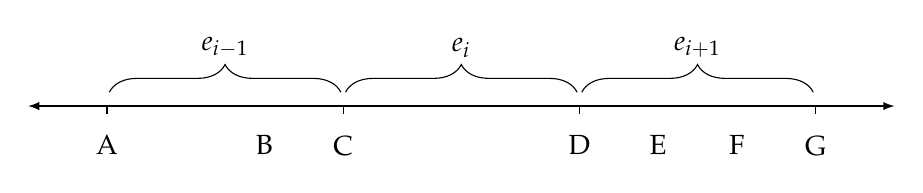
\begin{tikzpicture}
% axis
\draw[latex-latex] (0,0) -- (11,0) ;

% epoch braces
\draw [decorate,decoration={brace,amplitude=10pt} ,yshift=5pt] (1.03,0) -- (3.97,0)
  node [midway, above, yshift=9pt]{$e_{i-1}$};
\draw [decorate,decoration={brace,amplitude=10pt} ,yshift=5pt] (4.03,0) -- (6.97,0)
  node [midway, above, yshift=9pt]{$e_{i}$};
\draw [decorate,decoration={brace,amplitude=10pt} ,yshift=5pt] (7.03,0) -- (9.97,0)
  node [midway, above, yshift=9pt]{$e_{i+1}$};

% epoch boundaries
\foreach \x in  {1,4,7,10}
  \draw[shift={(\x,0)}] (0pt,0pt) -- (0pt,-3pt);

\node at (1,-0.5) {A};
\node at (3,-0.5) {B};
\node at (4,-0.5) {C};
\node at (7,-0.5) {D};
\node at (8,-0.5) {E};
\node at (9,-0.5) {F};
\node at (10,-0.5) {G};

\end{tikzpicture}

We must therefore store the last three stake distributions.
The mnemonic ``mark, set, go'' will be used to keep
track of the snapshots, where the label ``mark'' refers to the most recent snapshot,
and ``go'' refers to the snapshot that is ready to be used in the reward calculation.
In the above diagram, the snapshot taken at (A) is labeled ``mark'' during epoch $e_{i-1}$,
``set'' during epoch $e_i$ and ``go'' during epoch $e_{i+1}$. At (G) the snapshot
taken at (A) is no longer needed and will be discarded.

The two main transition systems in this section are:
\begin{itemize}
  \item The transition system named $\mathsf{EPOCH}$, which is defined in
    Section~\ref{sec:total-epoch}, covers what happens at the epoch boundary,
    such as at (A), (C), (D) and (G).
  \item The transition named $\mathsf{RUPD}$, which is defined in
    Section~\ref{sec:reward-update-trans}, covers the reward calculation that
    happens between (E) and (F).
\end{itemize}


\begin{note}
  Between time D and E we are concerned with chain growth and stability.
  Therefore this duration can be stated as 2k blocks (to state it in slots requires details about
  the particular version of the Ouroboros protocol). The duration between F and G is also 2k blocks.
  Between E and F a single honest block is enough to ensure a random nonce.
\end{note}

\subsection{Helper Functions and Accounting Fields}
\label{sec:stake-dist-helpers}

Figure~\ref{fig:funcs:epoch-helper-rewards} defines four helper functions needed
throughout the rest of the section.

\begin{itemize}
  \item The function $\fun{obligation}$ calculates the the minimal amount of coin needed to
    pay out all deposit refunds, as of the current slot.
  \item The function $\fun{poolRefunds}$ is used to calculate the total refunds
    that must be distributed for stake pools scheduled to retire.
    Note that this calculation takes a slot number corresponding to the epoch boundary slot
    when the calculation is performed.  The returned map maps pool operator hashkeys to the
    refunds, which will ultimately be returned to the registered reward account.
  \item The function $\fun{poolStake}$ filters the stake distribution to one stake pool.
\end{itemize}


%%
%% Figure - Helper Functions for Epoch Rules
%%
\begin{figure}[htb]
  \emph{Total possible refunds}
  \begin{align*}
    & \fun{obligation} \in \PParams \to \StakeCreds \to \StakePools \to \Slot \to \Coin \\
    & \obligation{pp}{stkCreds}{stpools}{cslot} =\\
    & \sum\limits_{(\_ \mapsto s) \in \var{stkCreds}}
      \refund{d_{\mathsf{val}}}{d_{\min}}{\lambda_d}{(\slotminus{cslot}{s})}
      + \sum\limits_{(\_ \mapsto s) \in \var{stpools}}
      \refund{p_{\mathsf{val}}}{p_{\min}}{\lambda_p}{(\slotminus{cslot}{s})} \\
    &
      \begin{array}{lr@{~=~}l}
        \where
          & \dval,~d_{\min},~\lambda_d
          & \fun{keyDeposit}~\var{pp},~\fun{keyMinRefund}~\var{pp},~\fun{keyDecayRate}~\var{pp}
          \\
          & p_{\mathsf{val}},~p_{\min},~\lambda_p
          & \fun{poolDeposit}~\var{pp},~\fun{poolMinRefund}~\var{pp},~\fun{poolDecayRate}~\var{pp}
      \end{array}\\
  \end{align*}
  \emph{Pool refunds}
  \begin{align*}
      & \fun{poolRefunds} \in \PParams \to (\KeyHash_{pool} \mapsto \Epoch) \to \Slot \to
      (\KeyHash_{pool} \mapsto \Coin) \\
      & \poolRefunds{pp}{retiring}{cslot} = \left\{
        \var{hk}\mapsto
          \refund{p_{\mathsf{val}}}{p_{\min}}{\lambda_p}{(\slotminus{cslot}{(\fun{slot}~e)})}
          \mid
          \var{hk}\mapsto e\in\var{retiring}
        \right\}\\
      & \where p_{\mathsf{val}},~p_{\min},~\lambda_p =
          \fun{poolDeposit}~\var{pp},~\fun{poolMinRefund}~\var{pp},~\fun{poolDecayRate}~\var{pp} \\
  \end{align*}

  \emph{Filter Stake to one Pool}
  \begin{align*}
      & \fun{poolStake} \in \KeyHash_{pool} \to (\KeyHash_{stake} \mapsto \KeyHash_{pool})
        \to \Stake \to \Stake \\
      & \poolStake{hk}{delegs}{stake} =
        \dom{(\var{delegs}\restrictrange\{hk\})\restrictdom\var{stake}}
  \end{align*}

  \caption{Helper Functions used in Rewards and Epoch Boundary}
  \label{fig:funcs:epoch-helper-rewards}
\end{figure}


The Figure~\ref{fig:defs:accounting} lists the accounting fields, denoted by $\Acnt$,
which will be used throughout this section. It consists of:
\begin{itemize}
  \item The value $\var{treasury}$ tracks the amount of coin currently stored in the treasury.
    Initially there will be no way to remove these funds.
  \item The value $\var{reserves}$ tracks the amount of coin currently stored in the reserves.
    This pot is used to pay rewards.
\end{itemize}
More will be said about the general accounting system in Section~\ref{sec:reward-calc}.

%%
%% Figure - Accounting fields
%%
\begin{figure}[htb]
  \emph{Accounting Fields}
  \begin{equation*}
    \Acnt =
    \left(
      \begin{array}{r@{~\in~}ll}
        \var{treasury} & \Coin & \text{treasury pot}\\
        \var{reserves} & \Coin & \text{reserve pot}\\
      \end{array}
    \right)
  \end{equation*}
  %
  \caption{Accounting fields}
  \label{fig:defs:accounting}
\end{figure}


\subsection{Stake Distribution Calculation}
\label{sec:stake-dist-calc}

This section defines the stake distribution calculations.
Figure~\ref{fig:epoch-defs} introduces three new derived types:
\begin{itemize}
  \item $\type{BlocksMade}$ represents the number of blocks each stake pool produced
    during an epoch.
  \item $\type{Stake}$ represents the amount of stake (in $\type{Coin}$) controlled by each
    stake pool.
\end{itemize}

%%
%% Figure - Epoch Abstract Types
%%
\begin{figure}[htb]
  \emph{Derived types}
  %
  \begin{equation*}
    \begin{array}{r@{~\in~}l@{\qquad=\qquad}lr}
      \var{blocks}
      & \BlocksMade
      & \KeyHash_{pool} \mapsto \N
      & \text{blocks made by stake pools} \\
      \var{stake}
      & \Stake
      & \Credential \mapsto \Coin
      & \text{stake} \\
    \end{array}
  \end{equation*}
  \caption{Epoch definitions}
  \label{fig:epoch-defs}
\end{figure}

The stake distribution calculation is given in Figure~\ref{fig:functions:stake-distribution}.

\begin{itemize}
\item $\fun{aggregate_{+}}$ takes a relation on $A\times B$, where $B$ is any
  monoid $(B,+,e)$ and returns a map from each $a\in A$ to the ``sum'' (using
  the monoidal $+$ operation) of all $b\in B$ such that $(a, b)\in A\times B$.
\item $\fun{stakeDistr}$ uses the $\fun{aggregate_{+}}$ function and several relations to
    compute the stake distribution, mapping each hashkey to the total coin under its control.
    Keys that are not both registered and delegated are filtered out.
    The relation passed to $\fun{aggregate_{+}}$ is made up of:
    \begin{itemize}
      \item $\fun{stakeCred_b}^{-1}$, relating credentials to (base) addresses
      \item $\left(\fun{addrPtr}\circ\var{ptr}\right)^{-1}$, relating credentials to (pointer)
        addresses
      \item $\range{utxo}$, relating addresses to coins
      \item $\fun{stakeCred_r}^{-1}\circ\var{rewards}$, relating (reward) addresses to coins
    \end{itemize}
    The notation for relations is explained in Section~\ref{sec:notation-shelley}.
\end{itemize}

%%
%% Figure Functions for Stake Distribution
%%
\begin{figure}[htb]
  \emph{Aggregation (for a monoid B)}
  %
  \begin{align*}
      & \fun{aggregate_{+}} \in \powerset{(A \times B)} \to (A\mapsto B) \\
      & \fun{aggregate_{+}}~\var{R} = \left\{a\mapsto \sum_{(a,b)\in\var{R}}b
          ~\mid~a\in\dom\var{R}\right\} \\
  \end{align*}
  %
  \emph{Stake Distribution (using functions and maps as relations)}
  %
  \begin{align*}
      & \fun{stakeDistr} \in \UTxO \to \DState \to \PState \to \Stake \\
      & \fun{stakeDistr}~{utxo}~{dstate}~{pstate} =
      (\dom{\var{activeDelegs}})\restrictdom\left(\fun{aggregate_{+}}~\var{stakeRelation}\right)\\
      & \where \\
      & ~~~~ (\var{stkCreds},~\var{rewards},~\var{delegations},~\var{ptrs},~\wcard,~\wcard)
        = \var{dstate} \\
      & ~~~~ (\var{stpools},~\wcard,~\wcard) = \var{pstate} \\
      & ~~~~ \var{stakeRelation} = \left(
        \left(\fun{stakeCred_b}^{-1}\cup\left(\fun{addrPtr}\circ\var{ptr}\right)^{-1}\right)
        \circ\left(\range{\var{utxo}}\right)
        \right)
        \cup \left(\fun{stakeCred_r}^{-1}\circ\var{rewards}\right) \\
      & ~~~~ \var{activeDelegs} =
               (\dom{stkCreds}) \restrictdom \var{delegations} \restrictrange (\dom{stpools}) \\
  \end{align*}

  \caption{Stake Distribution Function}
  \label{fig:functions:stake-distribution}
\end{figure}

\clearpage

\subsection{Snapshot Transition}
\label{sec:snapshots}

The state transition types for stake distribution snapshots are given in
Figure~\ref{fig:ts-types:snapshot}.
Each snapshot consists of:
\begin{itemize}
  \item $\var{stake}$, a stake distribution, which is defined in
    Figure~\ref{fig:epoch-defs} as a mapping of credentials to coin.
  \item $\var{delegations}$, a delegation map, mapping credentials to stake pools.
  \item $\var{poolParameters}$, storing the pool parameters of each stake pool.
\end{itemize}

The type $\type{\Snapshots}$ contains the
information needing to be saved on the epoch boundary:
\begin{itemize}
  \item $\var{pstake_{mark}}$, $\var{pstake_{set}}$ and $\var{pstake_{go}}$ are the three
    snapshots as explained in Section~\ref{sec:reward-overview}.
  \item $\var{feeSS}$ stores the fees and decayed deposit amounts at the epoch boundary.
\end{itemize}

%%
%% Figure - Snapshots Defs
%%
\begin{figure}[htb]
  \emph{Snapshot environment}
  \begin{equation*}
    \SnapshotEnv =
    \left(
      \begin{array}{r@{~\in~}ll}
        \var{pp} & \PParams & \text{protocol parameters}\\
        \var{dstate} & \DState & \text{delegation state}\\
        \var{pstate} & \PState & \text{pool state}\\
      \end{array}
    \right)
  \end{equation*}
  %
  \emph{Snapshots}
  \begin{equation*}
    \Snapshot =
    \left(
      \begin{array}{r@{~\in~}ll}
        \var{stake} & \Stake & \text{stake distribution}\\
        \var{delegations} & \Credential\mapsto\KeyHash_{pool}
                          & \text{stake delegations}\\
        \var{poolParameters} & \KeyHash_{pool} \mapsto \PoolParam & \text{pool parameters }\\
      \end{array}
    \right)
  \end{equation*}

  \begin{equation*}
    \Snapshots =
    \left(
      \begin{array}{r@{~\in~}ll}
        \var{pstake_{mark}} & \Snapshot & \text{newest stake}\\
        \var{pstake_{set}}  & \Snapshot & \text{middle stake}\\
        \var{pstake_{go}}   & \Snapshot & \text{oldest stake}\\
        \var{feeSS} & \Coin & \text{fee snapshot}\\
      \end{array}
    \right)
  \end{equation*}
  %
  \emph{Snapshot States}
  \begin{equation*}
    \SnapshotState =
    \left(
      \begin{array}{r@{~\in~}ll}
        \var{ss} & \Snapshots & \text{snapshots}\\
        \var{utxoSt} & \UTxOState & \text{utxo state}\\
      \end{array}
    \right)
  \end{equation*}
  %
  \emph{Snapshot transitions}
  \begin{equation*}
    \_ \vdash
    \var{\_} \trans{snap}{\_} \var{\_}
    \subseteq \powerset (\SnapshotEnv \times \SnapshotState \times \Epoch \times \SnapshotState)
  \end{equation*}
  %
  \caption{Snapshot transition-system types}
  \label{fig:ts-types:snapshot}
\end{figure}

The snapshot transition rule is given in Figure~\ref{fig:rules:snapshot}.
This transition has no preconditions and results in the following state change:

\begin{itemize}
  \item The oldest snapshot is replaced with the penultimate one.
  \item The penultimate snapshot is replaced with the newest one.
  \item The newest snapshot is replaced with one just calculated.
  \item The fees and decayed deposits are stored in $\var{feeSS}$. Note that this value will not
    change between epochs, unlike the $\var{fees}$ and $\var{deposits}$ values in the UTxO state.
  \item In the UTxO state, the decayed deposit amounts are moved from the deposit pot
    to the fee pool. Note that in the reward transition (Section~\ref{sec:reward-calc}),
    the value $\var{feeSS}$ will be removed from the fee pot in the UTxO state.
    The decay is calculated based on \textit{the first slot in the upcoming epoch}.
\end{itemize}

%%
%% Figure - Snapshot Rule
%%
\begin{figure}[htb]
  \begin{equation}\label{eq:snapshot}
    \inference[Snapshot]
    {
      {
      \begin{array}{r@{~\leteq~}l}
        (\var{stkCreds},~\wcard,~\var{delegations},~\wcard,~\wcard,~\wcard) & \var{dstate}\\
        (\var{stpools},~\var{poolParams},~\wcard) & \var{pstate}\\
        \var{stake} & \stakeDistr{utxo}{dstate}{pstate} \\
        \var{slot} & \firstSlot{e} \\
        \var{oblg} & \obligation{pp}{stkCreds}{stpools}{slot} \\
        \var{decayed} & \var{deposits} - \var{oblg} \\
      \end{array}
      }
    }
    {
      \begin{array}{r}
        \var{pp} \\
        \var{dstate} \\
        \var{pstate} \\
      \end{array}
      \vdash
      \left(
        \begin{array}{r}
          \var{pstake_{mark}}\\
          \var{pstake_{set}}\\
          \var{pstake_{go}}\\
          \var{feeSS} \\
          ~ \\
          \var{utxo} \\
          \var{deposits} \\
          \var{fees} \\
          \var{pup} \\
        \end{array}
      \right)
      \trans{snap}{e}
      \left(
        \begin{array}{r}
          \varUpdate{(\var{stake},~\var{delegations},~\var{poolParams})} \\
          \varUpdate{\var{pstake_{mark}}} \\
          \varUpdate{\var{pstake_{set}}} \\
          \varUpdate{\var{fees} + \var{decayed}} \\
          ~ \\
          \var{utxo} \\
          \varUpdate{\var{oblg}} \\
          \varUpdate{\var{fees} + \var{decayed}} \\
          \var{pup} \\
        \end{array}
      \right)
    }
  \end{equation}
  \caption{Snapshot Inference Rule}
  \label{fig:rules:snapshot}
\end{figure}

\clearpage

\subsection{Pool Reaping Transition}
\label{sec:pool-reap}

Figure~\ref{fig:ts-types:pool-reap} defines the types for the pool reap transition,
which is responsible for removing pools slated for retirement in the given epoch.

%%
%% Figure - Pool Reap Defs
%%
\begin{figure}[htb]
  \emph{Pool Reap State}
  \begin{equation*}
    \PlReapState =
    \left(
      \begin{array}{r@{~\in~}ll}
        \var{utxoSt} & \UTxOState & \text{utxo state}\\
        \var{acnt} & \Acnt & \text{accounting}\\
        \var{dstate} & \DState & \text{delegation state}\\
        \var{pstate} & \PState & \text{pool state}\\
      \end{array}
    \right)
  \end{equation*}
  %
  \emph{Pool Reap transitions}
  \begin{equation*}
    \_ \vdash \_ \trans{poolreap}{\_} \_ \in
    \powerset (\PParams \times \PlReapState \times \Epoch \times \PlReapState)
  \end{equation*}
  %
  \caption{Pool Reap Transition}
  \label{fig:ts-types:pool-reap}
\end{figure}


The pool-reap transition rule is given in Figure~\ref{fig:rules:pool-reap}.
This transition has no preconditions and results in the following state change:

\begin{itemize}
  \item For each retiring pool, the refund for the pool registration deposit is added to the
    pool's registered reward account, provided the reward account is still registered.
  \item The sum of all the refunds attached to unregistered reward accounts are added to the
    treasury.
  \item The deposit pool is reduced by the amount of claimed and unclaimed refunds.
  \item Any delegation to a retiring pool is removed.
  \item Each retiring pool is removed from all four maps in the pool state.
\end{itemize}

%%
%% Figure - Pool Reap Rule
%%
\begin{figure}[htb]
  \begin{equation}\label{eq:pool-reap}
    \inference[Pool-Reap]
    {
      {
      \begin{array}{r@{~\leteq~}l}
        \var{retired} & \dom{(\var{retiring}^{-1}~\var{e})} \\
        \var{pr} & \poolRefunds{pp}{(\var{retired}\restrictdom\var{stpools})}{(\firstSlot{e})} \\
        \var{rewardAcnts}
                 & \{\var{hk}\mapsto \fun{poolRAcnt}~\var{pool} \mid
                   \var{hk}\mapsto\var{pool} \in \var{retired}\restrictdom\var{poolParams} \} \\
        \var{rewardAcnts'} & \left\{
                        a \mapsto c
                        \mathrel{\Bigg|}
                        \begin{array}{r@{~\in~}l}
                          \var{hk} \mapsto c & \var{pr}, \\
                          \var{hk}\mapsto\var{a} & \var{rewardAcnts} \\
                        \end{array}
                      \right\} \\
        \var{refunds} & \dom{rewards}\restrictdom\var{rewardAcnts'} \\
        \var{mRefunds} & \dom{rewards}\subtractdom\var{rewardAcnts'} \\
        \var{refunded} & \sum\limits_{\wcard\mapsto c\in\var{refunds}} c \\
        \var{unclaimed} & \sum\limits_{\wcard\mapsto c\in\var{mRefunds}} c \\
      \end{array}
      }
    }
    {
      \var{pp}
      \vdash
      \left(
        \begin{array}{r}
          \var{utxo} \\
          \var{deposits} \\
          \var{fees} \\
          \var{ups} \\
          ~ \\
          \var{treasury} \\
          \var{reserves} \\
          ~ \\
          \var{stkCreds} \\
          \var{rewards} \\
          \var{delegations} \\
          \var{ptrs} \\
          \var{genDelegs} \\
          \var{i_{rwd}} \\
          ~ \\
          \var{stpools} \\
          \var{poolParams} \\
          \var{retiring} \\
        \end{array}
      \right)
      \trans{poolreap}{e}
      \left(
        \begin{array}{rcl}
          \var{utxo} \\
          \varUpdate{\var{deposits}}
          & \varUpdate{-}
          & \varUpdate{(\var{unclaimed} + \var{refunded})} \\
          \var{fees} \\
          \var{ups} \\
          ~ \\
          \varUpdate{\var{treasury}} & \varUpdate{+} & \varUpdate{\var{unclaimed}} \\
          \var{reserves} \\
          ~ \\
          \var{stkCreds} \\
          \varUpdate{\var{rewards}} & \varUpdate{\unionoverridePlus} & \varUpdate{\var{refunds}} \\
          \varUpdate{\var{delegations}} & \varUpdate{\subtractrange} & \varUpdate{\var{retired}} \\
          \var{ptrs} \\
          \var{genDelegs} \\
          \var{i_{rwd}}\\
          ~ \\
          \varUpdate{\var{retired}} & \varUpdate{\subtractdom} & \varUpdate{\var{stpools}} \\
          \varUpdate{\var{retired}} & \varUpdate{\subtractdom} & \varUpdate{\var{poolParams}} \\
          \varUpdate{\var{retired}} & \varUpdate{\subtractdom} & \varUpdate{\var{retiring}} \\
        \end{array}
      \right)
    }
  \end{equation}
  \caption{Pool Reap Inference Rule}
  \label{fig:rules:pool-reap}
\end{figure}

\clearpage

\subsection{Protocol Parameters Update Transition}
\label{sec:pparam-update}

Finally, reaching the epoch boundary may trigger a change in the protocol
parameters. The protocol parameters environment consists of the new
protocol parameters and the delegation and pool states.
The state change is a change of the $\UTxOState$, the $\Acnt$ states and the current $\PParams$.
The type of this state transition is given in Figure~\ref{fig:ts-types:new-proto-param}.

%%
%% Figure - New Proto Param Defs
%%
\begin{figure}[htb]
  \emph{New Proto Param environment}
  \begin{equation*}
    \NewPParamEnv =
    \left(
      \begin{array}{r@{~\in~}ll}
        \var{pp_{new}} & \PParams^? & \text{new protocol parameters}\\
        \var{dstate} & \DState & \text{delegation state}\\
        \var{pstate} & \PState & \text{pool state}\\
      \end{array}
    \right)
  \end{equation*}
  %
  \emph{New Proto Param States}
  \begin{equation*}
    \NewPParamState =
    \left(
      \begin{array}{r@{~\in~}ll}
        \var{utxoSt} & \UTxOState & \text{utxo state}\\
        \var{acnt} & \Acnt & \text{accounting}\\
        \var{pp} & \PParams & \text{current protocol parameters}\\
      \end{array}
    \right)
  \end{equation*}
  %
  \emph{New Proto Param transitions}
  \begin{equation*}
    \_ \vdash
    \var{\_} \trans{newpp}{\_} \var{\_}
    \subseteq \powerset (\NewPParamEnv \times \NewPParamState \times \Epoch \times \NewPParamState)
  \end{equation*}
  %
  \caption{New Proto Param transition-system types}
  \label{fig:ts-types:new-proto-param}
\end{figure}


Figure~\ref{fig:rules:new-proto-param} defines the new protocol parameter transition.
The transition has two rules, depending on whether or not the new protocol parameters
meet some requirements.
In particular, we require that the new parameters would not incur a debt of the system that
can not be covered by the reserves, and that the max block size is greater than the sum of the
max transaction size and the max header size.
If the requirements are met, the new protocol parameters are accepted, the proposal is reset,
and the reserves are adjusted to account for changes in the deposits.
Otherwise, the only change is that the proposal is reset.

Regarding adjusting the reserves for changes in the deposits, one of three things happens:

\begin{itemize}
  \item If the new protocol parameters mean that \textbf{fewer} funds are required in the
    deposit pot to cover all possible refunds, then the excess is moved to the reserves.

  \item If the new protocol parameters mean that \textbf{more} funds are required in the
    deposit pot to cover all possible refunds and the difference is \textbf{less} than
    the reserve pot, then funds are moved from the reserve pot to cover the difference.

  \item If the new protocol parameters mean that \textbf{more} funds are required in the
    deposit pot to cover all possible refunds and the difference is \textbf{more} than
    the reserve pot, then Rule~\ref{eq:new-pc-denied} meets the precondition and the
    only change of state is that the update proposals are reset.
\end{itemize}

Note that here, unlike most of the inference rules in this document,
the $\var{utxoSt'}$ and the $\var{acnt'}$ do not come from valid UTxO or
accounts transitions in the antecedent. We simply define the consequent
transition using these directly (instead of listing all the fields in both
states in the consequent transition). It is done this way here
for ease of reading.

%%
%% Figure - New Proto Param Rule
%%
\begin{figure}[htb]
  \begin{equation}\label{eq:new-pc-accepted}
    \hspace{-0.3cm}
    \inference[New-Proto-Param-Accept]
    {
      \var{pp_{new}}\neq\Nothing \\~\\
      {\begin{array}{rcl}
         \var{slot} & \leteq & \firstSlot{e} \\
         \var{oblg_{cur}} & \leteq & \obligation{pp}{stkCreds}{stpools}{slot} \\
         \var{oblg_{new}} & \leteq & \obligation{pp_{new}}{stkCreds}{stpools}{slot} \\
         \var{(\wcard,~\wcard,~\wcard,~\wcard,~\wcard,~\wcard,~\var{i_{rwd}})} &
                                                                                      \leteq
                              & \var{dstate}\\
         \var{diff} & \leteq & \var{oblg_{cur}} - \var{oblg_{new}}\\
         (\var{utxo},~\var{deposits},~\var{fees},~\var{ups}) & \leteq & \var{utxoSt} \\
         (\var{pup},~\var{aup},~\var{favs},~\var{avs}) & \leteq & \var{ups} \\
      \end{array}}
      \\~\\~\\
      \var{oblg_{cur}} = \var{deposits} \\
      \var{reserves} + \var{diff} \geq \sum\limits_{\wcard\mapsto\var{val}\in\var{i_{rwd}}} val \\
      \fun{maxTxSize}~\var{pp_{new}} + \fun{maxHeaderSize}~\var{pp_{new}} <
        \fun{maxBlockSize}~\var{pp_{new}}
      \\~\\
        \var{utxoSt'} \leteq
        \left(\var{utxo},~\varUpdate{oblg_{new}},~\var{fees}
        \left(\varUpdate{\emptyset},~\var{aup},~\var{favs},~\var{avs}\right)\right)
      \\~\\
      (\var{treasury},~\var{reserves})\leteq \var{acnt} \\
      \var{acnt'} \leteq (\var{treasury},~\varUpdate{reserves + diff}) \\
    }
    {
      \begin{array}{l}
        \var{pp_{new}}\\
        \var{dstate}\\
        \var{pstate}\\
      \end{array}
      \vdash
      \left(
        \begin{array}{r}
          \var{utxoSt} \\
          \var{acnt} \\
          \var{pp}
        \end{array}
      \right)
      \trans{newpp}{e}
      \left(
        \begin{array}{rcl}
          \varUpdate{utxoSt'}\\
          \varUpdate{acnt'} \\
          \varUpdate{\var{pp_{new}}} \\
        \end{array}
      \right)
    }
  \end{equation}

  \nextdef

  \begin{equation}\label{eq:new-pc-denied}
    \inference[New-Proto-Param-Denied]
    {
      \left({\begin{array}{c}
            \var{pp_{new}}=\Nothing \\
        \lor \\
        \var{reserves} + \var{diff} < \sum\limits_{\wcard\mapsto\var{val}\in\var{i_{rwd}}} val\\
        \lor \\
        \fun{maxTxSize}~\var{pp_{new}} + \fun{maxHeaderSize}~\var{pp_{new}} \geq
          \fun{maxBlockSize}~\var{pp_{new}}
      \end{array}}\right)
      \\~\\~\\
      {\begin{array}{rcl}
          \var{slot} & \leteq & \firstSlot{e} \\
          \var{oblg_{cur}} & \leteq & \obligation{pp}{stkCreds}{stpools}{slot} \\
          \var{oblg_{new}} & \leteq & \obligation{pp_{new}}{stkCreds}{stpools}{slot} \\
         \var{(\wcard,~\wcard,~\wcard,~\wcard,~\wcard,~\wcard,~\var{i_{rwd}})} &
                                                                                 \leteq
                              & \var{dstate}\\
         \var{diff} & \leteq & \var{oblg_{cur}} - \var{oblg_{new}}
      \end{array}}
      \\~\\~\\
      \left(\var{utxo},~\var{oblg},~\var{fees}
        \left(\var{pup},~\var{aup},~\var{favs},~\var{avs}\right)\right)
        \leteq \var{utxoSt} \\
        \var{utxoSt'} \leteq
        \left(\var{utxo},~\var{oblg},~\var{fees}
        \left(\varUpdate{\emptyset},~\var{aup},~\var{favs},~\var{avs}\right)\right)
    }
    {
      \begin{array}{l}
        \var{pp_{new}}\\
        \var{dstate}\\
        \var{pstate}\\
      \end{array}
      \vdash
      \left(
        \begin{array}{r}
          \var{utxoSt} \\
          \var{acnt} \\
          \var{pp}
        \end{array}
      \right)
      \trans{newpp}{e}
      \left(
        \begin{array}{rcl}
          \varUpdate{utxoSt'}\\
          \var{acnt} \\
          \var{pp}
        \end{array}
      \right)
    }
  \end{equation}
  \caption{New Proto Param Inference Rule}
  \label{fig:rules:new-proto-param}
\end{figure}

\clearpage

\subsection{Complete Epoch Boundary Transition}
\label{sec:total-epoch}

Finally, it is possible to define the complete epoch boundary transition type,
which is defined in Figure~\ref{fig:ts-types:epoch}.
The transition has no evironment.
The state is made up of the the accounting state, the snapshots, the ledger state and the
protocol parameters.
The transition uses a helper function $\fun{votedValue}$ which returns
the consensus value of update proposals in the event that consensus is met.
\textbf{Note that} $\fun{votedValue}$
\textbf{is only well-defined if } $\Quorum$
\textbf{is greater than half the number of core nodes, i.e.}
$\Quorum > |\var{genDelegs}|/2$ \textbf{.}

%%
%% Figure - Epoch Defs
%%
\begin{figure}[htb]
  \emph{Epoch States}
  \begin{equation*}
    \EpochState =
    \left(
      \begin{array}{r@{~\in~}ll}
        \var{acnt} & \Acnt & \text{accounting}\\
        \var{ss} & \Snapshots & \text{snapshots}\\
        \var{ls} & \LState & \text{ledger state}\\
        \var{prevPp} & \PParams & \text{previous protocol parameters}\\
        \var{pp} & \PParams & \text{protocol parameters}\\
      \end{array}
    \right)
  \end{equation*}
  %
  \emph{Epoch transitions}
  \begin{equation*}
    \vdash
    \var{\_} \trans{epoch}{\_} \var{\_}
    \subseteq \powerset (\EpochState \times \Epoch \times \EpochState)
  \end{equation*}
  %
  \emph{Accessor Functions}
  \begin{equation*}
    \begin{array}{r@{~\in~}lr}
      \fun{getIR} & \EpochState \to (\StakeCredential \mapsto \Coin)
                  & \text{get instantaneous rewards} \\
    \end{array}
  \end{equation*}
  %
  \emph{Helper Functions}
  \begin{align*}
      & \fun{votedValue} \in (\KeyHashGen\mapsto\PParamsUpdate) \to \PParamsUpdate^?\\
      & \fun{votedValue}~\var{vs} =
        \begin{cases}
          p & \exists p\in\range{vs}~(|vs\restrictrange p|\geq \Quorum) \\
          \Nothing & \text{otherwise} \\
        \end{cases}
  \end{align*}
  %
  \caption{Epoch transition-system types}
  \label{fig:ts-types:epoch}
\end{figure}


The epoch transition rule calls $\mathsf{SNAP}$, $\mathsf{POOLREAP}$ and $\mathsf{NEWPP}$
in sequence. It also stores the previous protocol parameters in $\var{prevPp}$.
The previous protocol parameters will be used for the reward calculation in the upcoming epoch,
note that they correspond to the epoch for which the rewards are being calculated.
Additionally, this transition also adopts the pool parameters $\var{fPoolParams}$
corresponding to the pool re-registration certificates which we submitted late in the ending epoch.
The ordering of these rules is important.
The stake pools which will be updated by $\var{fPoolParams}$ or
reaped during the $\mathsf{POOLREAP}$ transition must still be a
part of the new snapshot, and so $\mathsf{SNAP}$ must occur before these two actions.
Moreover, $\mathsf{SNAP}$ sets the deposit pot equal to current obligation,
which is a property that is preserved by $\mathsf{POOLREAP}$ and which
is necessary for the preservation of Ada property in the $ \mathsf{NEWPP}$ transition.

%%
%% Figure - Epoch Rule
%%
\begin{figure}[htb]
  \begin{equation}\label{eq:epoch}
    \inference[Epoch]
    {
      (\var{utxoSt},~(\var{dstate},~\var{pstate}))\leteq\var{ls} \\
      {
        \begin{array}{r}
          \var{pp}\\
          \var{dstate} \\
          \var{pstate} \\
        \end{array}
      }
      \vdash
      {
        \left(
          {
            \begin{array}{r}
              \var{ss} \\
              \var{utxoSt} \\
            \end{array}
          }
        \right)
      }
      \trans{\hyperref[fig:rules:snapshot]{snap}}{e}
      {
        \left(
          {
            \begin{array}{r}
              \var{ss'} \\
              \var{utxoSt'} \\
            \end{array}
          }
        \right)
      }
      \\~\\~\\
      (\var{stpools},~\var{poolParams},~\var{fPoolParams},~\var{retiring})\leteq\var{pstate}
      \\
      \var{pstate'}\leteq(\var{stpools},~\var{poolParams}\unionoverrideRight\var{fPoolParams},
      ~\emptyset,~\var{retiring})
      \\~\\~\\
      \var{pp}
      \vdash
      \left(
        {
          \begin{array}{r}
            \var{utxoSt'} \\
            \var{acnt} \\
            \var{dstate} \\
            \var{pstate'} \\
          \end{array}
        }
      \right)
      \trans{\hyperref[fig:rules:pool-reap]{poolreap}}{e}
      \left(
      {
        \begin{array}{rcl}
            \var{utxoSt''} \\
            \var{acnt'} \\
            \var{dstate'} \\
            \var{pstate''} \\
        \end{array}
      }
      \right)
      \\~\\~\\
      \var{(\wcard,~\wcard,~\wcard,~\var{pup})}\leteq\var{utxoSt'}\\
      \var{pp_{new}}\leteq\var{pp}\unionoverrideRight
      \fun{votedValue}~\var{pup}\\
      {
        \begin{array}{r}
          \var{pp_{new}}\\
          \var{dstate'}\\
          \var{pstate''}\\
        \end{array}
      }
      \vdash
      \left(
        {
          \begin{array}{r}
            \var{utxoSt''} \\
            \var{acnt'} \\
            \var{pp}\\
          \end{array}
        }
      \right)
      \trans{\hyperref[fig:rules:new-proto-param]{newpp}}{e}
      \left(
      {
        \begin{array}{rcl}
            \var{utxoSt'''} \\
            \var{acnt''} \\
            \var{pp'}\\
        \end{array}
      }
      \right)
      \\~\\~\\
      \var{ls}' \leteq (\var{utxoSt}''',~(\var{dstate}',~\var{pstate}''))
    }
    {
      \vdash
      \left(
      \begin{array}{r}
        \var{acnt} \\
        \var{ss} \\
        \var{ls} \\
        \var{prevPp} \\
        \var{pp} \\
      \end{array}
      \right)
      \trans{epoch}{e}
      \left(
      \begin{array}{rcl}
        \varUpdate{\var{acnt''}} \\
        \varUpdate{\var{ss'}} \\
        \varUpdate{\var{ls'}} \\
        \varUpdate{\var{pp}} \\
        \varUpdate{\var{pp'}} \\
      \end{array}
      \right)
    }
  \end{equation}
  \caption{Epoch Inference Rule}
  \label{fig:rules:epoch}
\end{figure}

\clearpage

\subsection{Rewards Distribution Calculation}
\label{sec:reward-dist}

This section defines the reward calculation for the proof of stake leader election.
Figure~\ref{fig:functions:rewards} defines the pool reward as described in section
5.5.2 of~\cite{delegation_design}.

\begin{itemize}
  \item The function $\fun{maxPool}$ gives the maximum reward a stake pool can receive in an epoch.
    This is a fraction of the total available rewards for the epoch.
    The result depends on the pool's relative stake, the pool's pledge and the following
    protocol parameters:
    \begin{itemize}
      \item $\var{a_0}$, the leader-stake influence
      \item $n_{opt}$, the optimal number of saturated stake pools
    \end{itemize}
  \item The function $\fun{poolReward}$ gives the total rewards available to be
    distributed to the members of the given pool. It depends on the protocol parameter $d$,
    the relative stake $\sigma$, the number $n$ of blocks the pool added to the chain and the
    total number $\overline{N}$ of blocks added to the chain in the last epoch.

\end{itemize}

%%
%% Figure - Functions for the Reward Calculation
%%
\begin{figure}[htb]
  \emph{Maximal Reward Function, called $f(s,\sigma)$ in section 5.5.2 of~\cite{delegation_design}}
  %
  \begin{align*}
      & \fun{maxPool} \in \PParams \to \Coin \to \unitInterval \to \unitInterval \to \Coin \\
      & \fun{maxPool}~\var{pp}~\var{R}~\sigma~\var{p_r} =
          ~~~\floor*{
             \frac{R}{1 + a_0}
             \cdot
             \left(
               \sigma' + p'\cdot a_0\cdot\frac{\sigma' - p'\frac{z_0-\sigma'}{z_0}}{z_0}
             \right)} \\
      & ~~~\where \\
      & ~~~~~~~a_0 = \fun{influence}~pp \\
      & ~~~~~~~n_{opt} = \fun{nopt}~pp \\
      & ~~~~~~~z_0 = 1/n_{opt} \\
      & ~~~~~~~\sigma'=\min(\sigma,~z_0) \\
      & ~~~~~~~p'=\min(p_r,~z_0) \\
  \end{align*}

  \emph{Actual Reward Function, called $\hat{f}$ in section 5.5.2 of~\cite{delegation_design}}
  %
  \begin{align*}
      & \fun{poolReward} \in \unitInterval \to \unitInterval \to \N \to \N \to \Coin \to \Coin \\
      & \poolReward{d}{\sigma}{n}{\overline{N}}{f} =
      \floor*{\overline{p}\cdot\var{f}}\\
      & ~~~\where \\
      & ~~~~~~~\overline{p} =
        \begin{cases}
          \frac{\beta}{\sigma} & \text{if } d < 0.8 \\
          1 & \text{otherwise}
        \end{cases} \\
      & ~~~~~~~\beta = \frac{n}{\max(1, \overline{N})} \\
  \end{align*}
  \caption{Functions used in the Reward Calculation}
  \label{fig:functions:rewards}
\end{figure}

\clearpage

Figure~\ref{fig:functions:reward-splitting} gives the calculation for
splitting the pool rewards with its members, as described in 6.5.2 of \cite{delegation_design}.
The portion of rewards allocated to the pool operator and owners is different
than that of the members.

\begin{itemize}
  \item The $\fun{r_{operator}}$ function calculates the leader reward, based on the pool cost,
    margin and the proportion of the pool's total stake.  Note that this reward will go to the
    reward account specified in the pool registration certificate.
  \item The $\fun{r_{member}}$ function calculates the member reward, proportionally to their
    stake after the cost and margin are removed.
\end{itemize}

%%
%% Figure - Functions for the Reward Splitting
%%
\begin{figure}[htb]
  \emph{Pool leader reward, from section 5.5.3 of \cite{delegation_design}}
  %
  \begin{align*}
      & \fun{r_{operator}} \in \Coin \to \PoolParam \to \unitInterval \to \unitIntervalNonNull \to \Coin \\
      & \lReward{\hat{f}}{pool}{s}{\sigma} =
        \begin{cases}
        \hat{f} & \hat{f} \leq c\\
        c + \floor*{(\hat{f} - c)\cdot\left(m + (1-m)\cdot\frac{s}{\sigma}\right) }&
        \text{otherwise.}
      \end{cases} \\
      & ~~~\where \\
      & ~~~~~~~c = \fun{poolCost}~pool \\
      & ~~~~~~~m = \fun{poolMargin}~pool \\
  \end{align*}

  \emph{Pool member reward, from section 5.5.3 of \cite{delegation_design}}
  %
  \begin{align*}
    & \fun{r_{member}} \in \Coin \to \PoolParam \to \unitInterval \to \unitIntervalNonNull \to \Coin \\
    & \mReward{\hat{f}}{pool}{t}{\sigma} =
      \begin{cases}
        0 & \hat{f} \leq c\\
        \floor*{(\hat{f} - c)\cdot(1-m)\cdot\frac{t}{\sigma}} &
        \text{otherwise.}
      \end{cases} \\
    & ~~~\where \\
    & ~~~~~~~c = \fun{poolCost}~pool \\
    & ~~~~~~~m = \fun{poolMargin}~pool \\
  \end{align*}

  \caption{Functions used in the Reward Splitting}
  \label{fig:functions:reward-splitting}
\end{figure}


Finally, the full reward calculation is presented in Figure~\ref{fig:functions:reward-calc}.
The calculation is done pool-by-pool.
\begin{itemize}
\item The $\fun{rewardOnePool}$ function calculates the rewards given out to
  each member of a given pool. The pool leader is identified by the stake
  credential of the pool operator. The function returns the rewards, calculated
  as follows:
    \begin{itemize}
      \item $\var{pstake}$, the total amount of stake controlled by the stake pool.
      \item $\var{ostake}$, the total amount of stake controlled by the stake pool operator
        and owners
      \item $\sigma$, the total proportion of stake controlled by the stake pool.
      \item $\overline{N}$, the expected number of blocks the pool should have produced.
      \item $\var{pledge}$, the pool's pledge in lovelace.
      \item $p_r$, the pool's pledge, as a proportion of active stake.
      \item $\var{maxP}$, maximum rewards the pool can claim if the pledge is met,
        and zero otherwise.
      \item $\var{poolR}$, the pool's actual reward, based on its performance.
      \item $\var{mRewards}$, the member's rewards as a mapping of reward accounts to coin.
      \item $\var{lReward}$, the leader's reward as coin.
      \item $\var{potentialRewards}$, the combination of $\var{mRewards}$ and $\var{lRewards}$.
      \item $\var{rewards}$, the restriction of $\var{potentialRewards}$ to the active
        reward accounts.
    \end{itemize}
  \item The $\fun{reward}$ function applies $\fun{rewardOnePool}$ to each registered stake pool.
\end{itemize}

%%
%% Figure - The Reward Calculation
%%
\begin{figure}[htb]
  \emph{Calculation to reward a single stake pool}
  %
  \begin{align*}
    & \fun{rewardOnePool} \in \PParams \to \Coin \to \N \to \N \to \KeyHash \to \PoolParam\\
      & ~~~\to \Stake \to \Coin \to \powerset{\AddrRWD}
           \to (\AddrRWD \mapsto \Coin) \\
      & \rewardOnePool{pp}{R}{n}{\overline{N}}{poolHK}{pool}{stake}{tot}{addrs_{rew}} =
          \var{rewards}\\
      & ~~~\where \\
      & ~~~~~~~\var{pstake} = \sum_{\_\mapsto c\in\var{stake}} c \\
      & ~~~~~~~\var{ostake} = \sum_{\substack{
        hk_\mapsto c\in\var{stake}\\
        hk\in(\fun{poolOwners}~\var{pool})\\
        }} c \\
      & ~~~~~~~\sigma = \var{pstake} / tot \\
      & ~~~~~~~\var{pledge} = \fun{poolPledge}~pool \\
      & ~~~~~~~p_{r} = \var{pledge} / \var{tot} \\
      & ~~~~~~~maxP =
      \begin{cases}
        \fun{maxPool}~\var{pp}~\var{R}~\sigma~\var{p_r}&
        \var{pledge} \leq \var{ostake}\\
        0 & \text{otherwise.}
      \end{cases} \\
      & ~~~~~~~\var{poolR} = \poolReward{(\fun{d}~pp)}{\sigma}{n}{\overline{N}}{maxP} \\
      & ~~~~~~~\var{mRewards} = \left\{
                                  \addrRw~hk\mapsto\mReward{poolR}{pool}{\frac{c}{tot}}{\sigma}
                                  ~\Big\vert~
                                  hk\mapsto c\in\var{stake},~~hk \neq\var{poolHK}
                               \right\}\\
      & ~~~~~~~\var{lReward} = \lReward{poolR}{pool}{\frac{\var{ostake}}{tot}}{\sigma} \\
      & ~~~~~~~\var{potentialRewards} =
                 \var{mRewards} \cup
                 \{(\fun{poolRAcnt}~\var{pool})\mapsto\var{lReward}\} \\
      & ~~~~~~~\var{rewards} = \var{addrs_{rew}}\restrictdom{\var{potentialRewards}} \\
  \end{align*}

  \emph{Calculation to reward all stake pools}
  %
  \begin{align*}
      & \fun{reward} \in \PParams \to \BlocksMade \to \Coin\to \powerset{\AddrRWD}
      \to (\KeyHash \mapsto \PoolParam) \\
      & ~~~\to \Stake \to (\KeyHash_{stake} \mapsto \KeyHash_{pool}) \to
      \Coin \to (\AddrRWD \mapsto \Coin)\\
      & \reward{pp}{blocks}{R}{addrs_{rew}}{poolParams}{stake}{delegs}{total}
          = \var{rewards}\\
      & ~~~\where \\
      & ~~~~~~~tot = \sum_{\_\mapsto c\in \var{stake}}c \\
      & ~~~~~~~\var{\overline{N}} = \sum_{\_\mapsto m\in blocks}m \\
      & ~~~~~~~pdata = \left\{
        hk\mapsto \left(p,~n,~\poolStake{hk}{delegs}{stake}\right)
        \mathrel{\Bigg|}
        \begin{array}{r@{\mapsto}c@{~\in~}l}
          hk & \var{p} & \var{poolParams} \\
          hk & \var{n} & \var{blocks} \\
        \end{array}
      \right\} \\
      & ~~~~~~~\var{results} = \left\{
        hk \mapsto \rewardOnePool{pp}{R}{n}{\overline{N}}{hk}{p}{s}{tot}{addrs_{rew}}
                 \mid
        hk\mapsto(p, n, s)\in\var{pdata} \right\} \\
      & ~~~~~~~\var{rewards} = \bigcup_{\wcard\mapsto\var{r}\in\var{results}}\var{r}
  \end{align*}
  \caption{The Reward Calculation}
  \label{fig:functions:reward-calc}
\end{figure}

\clearpage

\subsection{Reward Update Calculation}
\label{sec:reward-calc}

This section defines the calculation of a reward update.
A reward update is the information needed to account for the movement of lovelace
in the system due to paying out rewards.

Figure~\ref{fig:fund-preservation} captures the potential movement of funds in the entire system,
taking every transition system in this document into account.  Value is moved between
accounting pots, but the total amount of value in the system remains constant.
In particular, the red subgraph represents the inputs and outputs to
the ``reward pot'', a temporary variable used during the reward update calculation in
Figure~\ref{fig:functions:reward-update-creation}.
The blue arrows represent the movement of funds that pass through the ``reward pot''.


\begin{figure}[htb]
  \begin{center}
    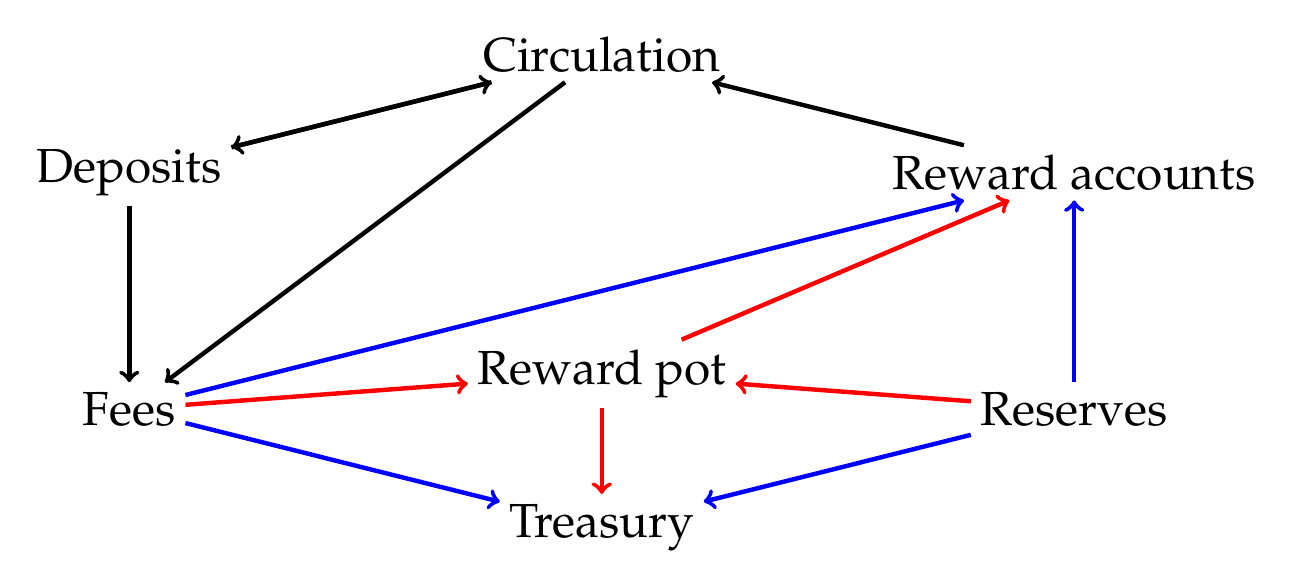
\begin{tikzpicture}
      [ x=30mm, y=30mm
      , direct/.style={black, draw}
      , implied/.style={blue, draw}
      , toTotPot/.style={red, draw}
      ]
    \node (C) at (3,2.5) {\LARGE Circulation};
    \node (R) at (5, 1) {\LARGE Reserves};
    \node (D) at (1, 2) {\LARGE Deposits};
    \node (FR) at (1,1) {\LARGE Fees};
    \node (RA) at (5, 2) {\LARGE Reward accounts};
    \node (T) at (3,0.5) {\LARGE Treasury};

    \draw[->, direct, ultra thick]
    (C) edge (D)
    (C) edge (FR)

    (D) edge (C)
    (D) edge (FR)

    (RA) edge (C);

    \draw[->, implied, ultra thick]
    (FR) edge (T)
    (FR) edge (RA)

    (R) edge (T)
    (R) edge (RA);

    \node (TP) at (3, 1.15) {\LARGE Reward pot};

    \draw[->, toTotPot, ultra thick]
    (FR) edge (TP)
    (R) edge (TP)

    (TP) edge (RA)
    (TP) edge (T);
    \end{tikzpicture}
  \end{center}
  \caption{Preservation of Value}
  \label{fig:fund-preservation}
\end{figure}

Figure~\ref{fig:defs:reward-update} defines a reward update.
It consists of four pots:
\begin{itemize}
  \item The change to the treasury. This will be a positive value.
  \item The change to the reserves. This will be a negative value.
  \item The map of new individual rewards (to be added to the existing rewards).
  \item The change to the fee pot. This will be a negative value.
    rewards.
\end{itemize}

%%
%% Figure - Reward Update Defs
%%
\begin{figure}[htb]
  \emph{Reward Update}
  \begin{equation*}
    \RewardUpdate =
    \left(
      \begin{array}{r@{~\in~}ll}
        \Delta t & \Coin & \text{change to the treasury} \\
        \Delta r & \Coin & \text{change to the reserves} \\
        \var{rs} & \AddrRWD\mapsto\Coin & \text{new individual rewards} \\
        \Delta f & \Coin & \text{change to the fee pot} \\
      \end{array}
    \right)
  \end{equation*}
  %
  \caption{Rewards Update type}
  \label{fig:defs:reward-update}
\end{figure}

\clearpage

Figure~\ref{fig:functions:reward-update-creation} defines two functions,
$\fun{createRUpd}$ to create a reward update and $\fun{applyRUpd}$ to apply a
reward update to an instance of $\EpochState$.

The $\fun{createRUpd}$ function does the following:
\begin{itemize}
  \item Note that for all the calculations below, we use the previous protocol parameters
    $\var{prevPp}$, which corresponds to the parameters during the epoch for which we
    are creating rewards.
  \item First we calculate the change to the reserves,
    as determined by the $\rho$ protocol parameter.
  \item Next we calculate $\var{rewardPot}$, the total amount of coin available for rewards this
    epoch, as described in section 6.4 of \cite{delegation_design}. It consists of four pots:
    \begin{itemize}
      \item The fee pot, containing the transaction fees from the epoch.
      \item The amount of coin in the deposit pot that is no longer needed, due to decay.
      \item The amount of monetary expansion from the reserves, calculated above.
    \end{itemize}
    Note that the fee pot and the decayed amount are taken from the snapshot taken at the
    epoch boundary.  (See~Figure\ref{fig:rules:snapshot}).
  \item Next we calculate the proportion of the reward pot that will move to the treasury,
    as determined by the $\tau$ protocol parameter. The remaining pot is called the
    $\var{R}$, just as in section 6.5 of \cite{delegation_design}.
  \item The rewards are calculated, using the oldest stake distribution snapshot (the one
    labeled ``go'').
    As given by $\fun{maxPool}$, each pool can receive a maximal amount, determined by its
    performance.  The difference between the maximal amount and the actual amount received is
    added to the amount moved to the treasury.
  \item The fee pot will be reduced by $\var{feeSS}$.
\end{itemize}

Note that fees are not explicitly removed from any account:
the fees come from transactions paying them and are accounted for whenever
transactions are processed and when the deposit decay value comes from returning
smaller refunds for deposits than were paid upon depositing.

The $\fun{applyRUpd}$ function does the following:
    \begin{itemize}
      \item Adjust the treasury, reserves and fee pots by the appropriate amounts.
      \item Add each individual reward to the global reward mapping.
    \end{itemize}

These two functions will be used in the blockchain transition systems in Section~\ref{sec:chain}.
In particular,
$\fun{createRUpd}$ will be used in Equation~\ref{eq:reward-update},
and $\fun{applyRUpd}$ will be used in Equation~\ref{eq:new-epoch}.

%%
%% Figure - The Reward Update Creation
%%
\begin{figure}[htb]
  \emph{Calculation to create a reward update}
  %
  \begin{align*}
    & \fun{createRUpd} \in \BlocksMade \to \EpochState \to \Coin \to \RewardUpdate \\
    & \createRUpd{b}{es}{total} = \left(
      \Delta t_1+\Delta t_2,-~\Delta r,~\var{rs},~-\var{feeSS}\right) \\
    & ~~~\where \\
    & ~~~~~~~(\var{acnt},~\var{ss},~\var{ls},~\var{prevPp},~\wcard) = \var{es} \\
    & ~~~~~~~(\wcard,~\wcard,~\var{pstake_{go}},~\var{poolsSS},~\var{feeSS}) = \var{ss}\\
    & ~~~~~~~(\var{stake},~\var{delegs}) = \var{pstate_{go}} \\
    & ~~~~~~~(\wcard,~\var{reserves}) = \var{acnt} \\
    & ~~~~~~~\left(
      \wcard,~
      \left(
      \left(\wcard,~\var{rewards},~\wcard,~\wcard,~\wcard,~\wcard\right)~
      \wcard
      \right)
      \right) = \var{ls} \\
    & ~~~~~~~\Delta r = \floor*{\min(1,\eta) \cdot (\fun{rho}~\var{prevPp}) \cdot
      \var{reserves}}
    \\
    & ~~~~~~~\eta = \frac{blocksMade}{\SlotsPerEpoch \cdot \ActiveSlotCoeff} \\
    & ~~~~~~~\var{rewardPot} = \var{feeSS} + \Delta r \\
    & ~~~~~~~\Delta t_1 = \floor*{(\fun{tau}~\var{prevPp}) \cdot \var{rewardPot}} \\
    & ~~~~~~~\var{R} = \var{rewardPot} - \Delta t_1 \\
    & ~~~~~~~\var{circulation} = \var{total} - \var{reserves} \\
    & ~~~~~~~\var{rs}
      = \reward{prevPp}{b}{R}{(\dom{rewards})}{poolsSS}{stake}{delegs}{circulation} \\
    & ~~~~~~~\Delta t_{2} = R - \left(\sum\limits_{\_\mapsto c\in\var{rs}}c\right) \\
    & ~~~~~~~blocksMade = \sum_{\wcard \mapsto m \in b}m
  \end{align*}

  \caption{Reward Update Creation}
  \label{fig:functions:reward-update-creation}
\end{figure}

\begin{figure}[htb]
  \emph{Applying a reward update}
  %
  \begin{align*}
      & \fun{applyRUpd} \in \RewardUpdate \to \EpochState \to \EpochState \\
      & \fun{applyRUpd}~
      \left(
        \begin{array}{c}
          \Delta t \\
          \Delta r \\
          \var{rs} \\
          \Delta f \\
        \end{array}
    \right)
      \left(
        \begin{array}{c}
          \var{treasury} \\
          \var{reserves} \\
          ~ \\
          \var{stkCreds} \\
          \var{rewards} \\
          \var{delegations} \\
          \var{ptrs} \\
          \var{genDelegs} \\
          \var{i_{rwd}}
          \\~ \\
          \var{stpools} \\
          \var{poolParams} \\
          \var{retiring} \\
          ~ \\
          \var{utxo} \\
          \var{deposits} \\
          \var{fees} \\
          \var{up} \\
          ~ \\
          \var{prevPp} \\
          \var{pp} \\
        \end{array}
      \right)
      =
      \left(
        \begin{array}{c}
          \varUpdate{\var{treasury} + \Delta t}\\
          \varUpdate{\var{reserves} + \Delta r}\\
          ~ \\
          \var{\var{stkCreds}} \\
          \varUpdate{\var{rewards}\unionoverridePlus\var{rs}} \\
          \var{delegations} \\
          \var{ptrs} \\
          \var{genDelegs} \\
          \var{i_{rwd}}
          \\~ \\
          \var{stpools} \\
          \var{poolParams} \\
          \var{retiring} \\
          ~ \\
          \var{utxo} \\
          \var{deposits} \\
          \varUpdate{\var{fees}+\Delta f} \\
          \var{up} \\
          ~ \\
          \var{prevPp} \\
          \var{pp} \\
        \end{array}
    \right)
  \end{align*}

  \caption{Reward Update Application}
  \label{fig:functions:reward-update-application}
\end{figure}

\clearpage

\section{Blockchain layer}
\label{sec:chain}

This chapter introduces the view of the blockchain layer as required for the
ledger. This includes in particular the information required for the epoch
boundary and its rewards calculation as described in Section~\ref{sec:epoch}. It
also covers the transitions that keep track of produced blocks in order to
calculate rewards and penalties for stake pools.

The main transition rule is $\mathsf{CHAIN}$ which calls the subrules
$\mathsf{NEWEPOCH}$ and $\mathsf{UPDN}$, $\mathsf{VRF}$ and $\mathsf{BBODY}$.

\subsection{Block Definitions}
\label{sec:defs-blocks}

\begin{figure*}[htb]
  \emph{Abstract types}
  %
  \begin{equation*}
    \begin{array}{r@{~\in~}lr}
      \var{h} & \HashHeader & \text{hash of a block header}\\
      \var{hb} & \HashBBody & \text{hash of a block body}\\
      \var{bn} & \BlockNo & \text{block number}\\
    \end{array}
  \end{equation*}
  %
  \emph{Operational Certificate}
  %
  \begin{equation*}
    \OCert =
    \left(
      \begin{array}{r@{~\in~}lr}
        \var{vk_{hot}} & \VKeyEv & \text{operational (hot) key}\\
        \var{n} & \N & \text{certificate issue number}\\
        c_0 & \KESPeriod & \text{start KES period}\\
        \sigma & \Sig & \text{cold key signature}\\
      \end{array}
    \right)
  \end{equation*}
  %
  \emph{Block Header Body}
  %
  \begin{equation*}
    \BHBody =
    \left(
      \begin{array}{r@{~\in~}lr}
        \var{prev} & \HashHeader^? & \text{hash of previous block header}\\
        \var{vk} & \VKey & \text{block issuer}\\
        \var{vrfVk} & \VKey & \text{VRF verification key}\\
        \var{blockno} & \BlockNo & \text{block number}\\
        \var{slot} & \Slot & \text{block slot}\\
        \eta & \Seed & \text{nonce}\\
        \var{prf}_{\eta} & \Proof & \text{nonce proof}\\
        \ell & \unitInterval & \text{leader election value}\\
        \var{prf_{\ell}} & \Proof & \text{leader election proof}\\
        \var{bsize} & \N & \text{size of the block body}\\
        \var{bhash} & \HashBBody & \text{block body hash}\\
        \var{oc} & \OCert & \text{operational certificate}\\
        \var{pv} & \ProtVer & \text{protocol version}\\
      \end{array}
    \right)
  \end{equation*}
  %
  \emph{Block Types}
  %
  \begin{equation*}
    \begin{array}{r@{~\in~}l@{\qquad=\qquad}l}
      \var{bh}
      & \BHeader
      & \BHBody \times \Sig
      \\
      \var{b}
      & \Block
      & \BHeader \times \seqof{\Tx}
    \end{array}
  \end{equation*}
  \emph{Abstract functions}
  %
  \begin{equation*}
    \begin{array}{r@{~\in~}lr}
      \bhHash{} & \BHeader \to \HashHeader
                   & \text{hash of a block header} \\
      \bHeaderSize{} & \BHeader \to \N
                   & \text{size of a block header} \\
      \bBodySize{} & \seqof{\Tx} \to \N
                   & \text{size of a block body} \\
      \slotToSeed{} & \Slot \to \Seed
                    & \text{convert a slot to a seed} \\
      \prevHashToNonce{} & \HashHeader^? \to \Seed
                    & \text{convert an optional header hash to a seed} \\
      \fun{bbodyhash} & \seqof{\Tx} \to \HashBBody \\
    \end{array}
  \end{equation*}
  %
  \emph{Accessor Functions}
  \begin{equation*}
    \begin{array}{r@{~\in~}l@{~~~~~~~~~~}r@{~\in~}lr}
      \fun{bheader} & \Block \to \BHeader &
      \fun{bhbody} & \BHeader \to \BHBody \\
      \fun{hsig} & \BHeader \to \Sig &
      \fun{bbody} & \Block \to \seqof{\Tx} \\
      \fun{bvkcold} & \BHBody \to \VKey &
      \fun{bvkvrf} & \BHBody \to \VKey \\
      \fun{bprev} & \BHBody \to \HashHeader^? &
      \fun{bslot} & \BHBody \to \Slot \\
      \fun{bblockno} & \BHBody \to \BlockNo &
      \fun{bnonce} & \BHBody \to \Seed \\
      \fun{\bprfn{}} & \BHBody \to \Proof &
      \fun{bleader} & \BHBody \to \N \\
      \fun{\bprfl{}} & \BHBody \to \Proof &
      \fun{hBbsize} & \BHBody \to \N \\
      \fun{bhash} & \BHBody \to \HashBBody &
      \fun{bocert} & \BHBody \to \OCert \\
    \end{array}
  \end{equation*}
  %
  \caption{Block Definitions}
  \label{fig:defs:blocks}
\end{figure*}

\clearpage

\subsection{MIR Transition}
\label{sec:mir-trans}

The transition which moves the instantaneous rewards is $\mathsf{MIR}$.
Figure~\ref{fig:ts-types:mir} defines the types for the transition.
It has no environment or signal, and the state is $\EpochState$.

\begin{figure}
  \emph{MIR Transitions}
  \begin{equation*}
    \vdash \var{\_} \trans{mir}{} \var{\_} \subseteq
    \powerset (\EpochState \times \EpochState)
  \end{equation*}
  \caption{MIR transition-system types}
  \label{fig:ts-types:mir}
\end{figure}

Figure~\ref{fig:rules:mir} defines the MIR state transition.

If the reserve and treasury pots are large enough to cover the sum
of the corresponding instantaneous rewards,
the reward accounts are increased by the appropriate amount
and the two pots are decreased appropriately.
In either case, if the pots are large enough or not,
we reset both of the instantaneous reward mappings back to the empty mapping.

\begin{figure}[ht]
  \begin{equation}\label{eq:mir}
    \inference[MIR]
    {
      (\var{rewards},~\var{delegations},~
      \var{ptrs},~\var{fGenDelegs},~\var{genDelegs},~\var{i_{rwd}})
        \leteq \var{ds}
      \\
      (\var{treasury},~\var{reserves})\leteq\var{acnt}
      &
      (\var{irReserves},~\var{irTreasury})\leteq\var{i_{rwd}}
      \\~\\
      \var{irwdR}\leteq
        \left\{
        \fun{addr_{rwd}}~\var{hk}\mapsto\var{val}
        ~\vert~\var{hk}\mapsto\var{val}\in(\dom{rewards})\restrictdom\var{irReserves}
        \right\}
      \\
      \var{irwdT}\leteq
        \left\{
        \fun{addr_{rwd}}~\var{hk}\mapsto\var{val}
        ~\vert~\var{hk}\mapsto\var{val}\in(\dom{rewards})\restrictdom\var{irTreasury}
        \right\}
      \\~\\
      \var{totR}\leteq\sum\limits_{\wcard\mapsto v\in\var{irwdR}}v
      &
      \var{totT}\leteq\sum\limits_{\wcard\mapsto v\in\var{irwdT}}v
      \\
      \var{totR}\leq\var{reserves}
      &
      \var{totT}\leq\var{treasury}
      \\~\\
      \var{rewards'}\leteq\var{rewards}\unionoverridePlus\var{irwdR}\unionoverridePlus\var{irwdT}
      \\
      \var{ds'} \leteq
      (\varUpdate{\var{rewards}'},~\var{delegations},~
      \var{ptrs},~\var{fGenDelegs},~\var{genDelegs},
      ~(\varUpdate{\emptyset},~\varUpdate{\emptyset}))
    }
    {
      \vdash
      {\left(\begin{array}{c}
            \var{acnt} \\
            \var{ss} \\
            (\var{us},~(\var{ds},~\var{ps})) \\
            \var{prevPP} \\
            \var{pp} \\
      \end{array}\right)}
      \trans{mir}{}
      {\left(\begin{array}{c}
            \varUpdate{(\varUpdate{\var{treasury}-\var{totT}},~\varUpdate{\var{reserves}-\var{totR}})} \\
            \var{ss} \\
            (\var{us},~(\varUpdate{\var{ds'}},~\var{ps})) \\
            \var{prevPP} \\
            \var{pp} \\
      \end{array}\right)}
    }
  \end{equation}

  \nextdef

  \begin{equation}\label{eq:mir-skip}
    \inference[MIR-Skip]
    {
      (\var{rewards},~\var{delegations},~
      \var{ptrs},~\var{fGenDelegs},~\var{genDelegs},~\var{i_{rwd}})
        \leteq \var{ds}
      \\
      (\var{treasury},~\var{reserves})\leteq\var{acnt}
      &
      (\var{irReserves},~\var{irTreasury})\leteq\var{i_{rwd}}
      \\~\\
      \var{irwdR}\leteq
        \left\{
        \fun{addr_{rwd}}~\var{hk}\mapsto\var{val}
        ~\vert~\var{hk}\mapsto\var{val}\in(\dom{rewards})\restrictdom\var{irReserves}
        \right\}
      \\
      \var{irwdT}\leteq
        \left\{
        \fun{addr_{rwd}}~\var{hk}\mapsto\var{val}
        ~\vert~\var{hk}\mapsto\var{val}\in(\dom{rewards})\restrictdom\var{irTreasury}
        \right\}
      \\~\\
      \var{totR}\leteq\sum\limits_{\wcard\mapsto v\in\var{irwdR}}v
      &
      \var{totT}\leteq\sum\limits_{\wcard\mapsto v\in\var{irwdT}}v
      \\
      \var{totR}>\var{reserves}~\lor~\var{totT}>\var{treasury}
      \\~\\
      \var{ds'} \leteq
      (\var{rewards},~\var{delegations},~
      \var{ptrs},~\var{fGenDelegs},~\var{genDelegs},
      ~(\varUpdate{\emptyset},~\varUpdate{\emptyset}))
    }
    {
      \vdash
      {\left(\begin{array}{c}
            \var{acnt} \\
            \var{ss} \\
            (\var{us},~(\var{ds},~\var{ps})) \\
            \var{prevPP} \\
            \var{pp} \\
      \end{array}\right)}
      \trans{mir}{}
      {\left(\begin{array}{c}
            \var{acnt} \\
            \var{ss} \\
            (\var{us},~(\varUpdate{\var{ds'}},~\var{ps})) \\
            \var{prevPP} \\
            \var{pp} \\
      \end{array}\right)}
    }
  \end{equation}
  \caption{MIR rules}
  \label{fig:rules:mir}
\end{figure}

\subsection{New Epoch Transition}
\label{sec:new-epoch-trans}

For the transition to a new epoch ($\mathsf{NEWEPOCH}$), the environment is
given in Figure~\ref{fig:ts-types:newepoch}, it consists of

\begin{itemize}
\item The current slot.
\item The set of genesis keys.
\end{itemize}
The new epoch state is given in Figure~\ref{fig:ts-types:newepoch}, it consists
of

\begin{itemize}
\item The number of the last epoch.
\item The information about produced blocks for each stake pool during the previous epoch.
\item The information about produced blocks for each stake pool during the current epoch.
\item The old epoch state.
\item An optional rewards update.
\item The stake pool distribution of the epoch.
\end{itemize}

\begin{figure}
  \emph{New Epoch states}
  \begin{equation*}
    \NewEpochState =
    \left(
      \begin{array}{r@{~\in~}lr}
        \var{e_\ell} & \Epoch & \text{last epoch} \\
        \var{b_{prev}} & \BlocksMade & \text{blocks made last epoch} \\
        \var{b_{cur}} & \BlocksMade & \text{blocks made this epoch} \\
        \var{es} & \EpochState & \text{epoch state} \\
        \var{ru} & \RewardUpdate^? & \text{reward update} \\
        \var{pd} & \PoolDistr & \text{pool stake distribution} \\
      \end{array}
    \right)
  \end{equation*}
  %
  \emph{New Epoch Transitions}
  \begin{equation*}
    \vdash \var{\_} \trans{newepoch}{\_} \var{\_} \subseteq
    \powerset (\NewEpochState \times \Epoch \times \NewEpochState)
  \end{equation*}
  %
  \emph{Helper function}
  \begin{align*}
      & \fun{calculatePoolDistr} \in \Snapshot \to \PoolDistr \\
      & \fun{calculatePoolDistr}~(\var{stake},~\var{delegs},~\var{poolParams}) = \\
      & ~~~\left\{\var{hk_p}\mapsto(\sigma,~\fun{poolVRF}~\var{p})
            ~\Big\vert~
            {
              \begin{array}{r@{~\in~}l}
                \var{hk_p}\mapsto\sigma & \var{sd} \\
                \var{hk_p}\mapsto\var{p} & \var{poolParams}
              \end{array}
            }
            \right\}\\
      & ~~~~\where \\
      & ~~~~~~~~~\var{total} = \sum_{\_ \mapsto c\in\var{stake}} c \\
      & ~~~~~~~~~\var{sd} = \fun{aggregate_{+}}~\left(\var{delegs}^{-1}\circ
                     \left\{\left(
                       \var{hk}, \frac{\var{c}}{\var{total}}
                     \right) \vert (\var{hk},
                     \var{c}) \in \var{stake}
                     \right\}\right) \\
  \end{align*}

  \caption{NewEpoch transition-system types}
  \label{fig:ts-types:newepoch}
\end{figure}

Figure~\ref{fig:rules:new-epoch} defines the new epoch state transition. It has three rules.
The first rule describes the change in the case of $e$ being equal to the next epoch $e_\ell+ 1$.
It also calls the $\mathsf{MIR}$ and $\mathsf{EPOCH}$ rules and checks that the reward update
is net neutral with respect to the Ada in the system.
This should always hold (by the definition of the $\fun{createRUpd}$ function)
and is present only for extra assurance and for help in proving
that Ada is preserved by this transition.
The second rule deals with the case when the epoch signal $e$ is not one greater than the
current epoch \var{e_\ell}. This rule does not change the state.
The third rule is nearly the same as the first rule, only there is no reward update to apply.
This third rule is defined for completeness, but in practice we hope that it is never used,
since it only applies in the case that epoch $e$ processed no blocks after the first
$\StabilityWindow$-many slots.

In the first case, the new epoch state is updated as follows:

\begin{itemize}
\item The epoch is set to the new epoch $e$.
\item The mapping for the blocks produced by each stake pool for the previous epoch
  is set to the current such mapping.
\item The mapping for the blocks produced by each stake pool for the current epoch
  is set to the empty map.
\item The epoch state is updated with: first applying the rewards update \var{ru},
  then calling the $\mathsf{MIR}$ transition, and finally by calling the
  $\mathsf{EPOCH}$ transition.
\item The rewards update is set to \Nothing.
\item The new pool distribution \var{pd}' is calculated from the delegation map and
  stake allocation of the previous epoch.
\end{itemize}

\begin{figure}[ht]
  \begin{equation}\label{eq:new-epoch}
    \inference[New-Epoch]
    {
      e = e_\ell + 1
      &
      \var{ru} \neq \Nothing
      &
      (\Delta t,~\Delta r,~\var{rs},~\Delta f)\leteq\var{ru}
      \\
      \Delta t+~\Delta r+\left(\sum\limits_{\wcard\mapsto v\in\var{rs}} v\right)+\Delta f=0
      \\
      \var{es'}\leteq\fun{applyRUpd}~\var{ru}~\var{es}
      &
      {
        \vdash
        \var{es'}
          \trans{\hyperref[fig:rules:mir]{mir}}{}\var{es''}
      }
      &
      {
        \vdash
        \var{es''}
          \trans{\hyperref[fig:rules:epoch]{epoch}}{\var{e}}\var{es'''}
      }
      \\~\\
      {\begin{array}{r@{~\leteq~}l}
         (\var{acnt},~\var{ss},~\wcard,~\wcard,~\wcard) & \var{es'''} \\
         (\wcard,~\var{pstake_{set}},~\wcard,~\wcard) & \var{ss} \\
         \var{pd'} & \fun{calculatePoolDistr}~\var{pstake_{set}} \\
       \end{array}}
    }
    {
      \vdash
      {\left(\begin{array}{c}
            \var{e_\ell} \\
            \var{b_{prev}} \\
            \var{b_{cur}} \\
            \var{es} \\
            \var{ru} \\
            \var{pd} \\
      \end{array}\right)}
      \trans{newepoch}{\var{e}}
      {\left(\begin{array}{c}
            \varUpdate{\var{e}} \\
            \varUpdate{\var{b_{cur}}} \\
            \varUpdate{\emptyset} \\
            \varUpdate{\var{es'''}} \\
            \varUpdate{\Nothing} \\
            \varUpdate{\var{pd}'} \\
      \end{array}\right)}
    }
  \end{equation}

  \nextdef

  \begin{equation}\label{eq:not-new-epoch}
    \inference[Not-New-Epoch]
    {
      (e_\ell,~\wcard,~\wcard,~\wcard,~\wcard,~\wcard,~\wcard)\leteq\var{nes}
      &
      e \neq e_\ell + 1
    }
    {
      \vdash\var{nes}\trans{newepoch}{\var{e}} \var{nes}
    }
  \end{equation}

  \nextdef

  \begin{equation}\label{eq:no-reward-update}
    \inference[No-Reward-Update]
    {
      (e_\ell,~\wcard,~\wcard,~\wcard,~\var{ru},~\wcard,~\wcard)\leteq\var{nes}
      &
      e = e_\ell + 1
      &
      \var{ru} = \Nothing
      \\
      {
        \vdash
        \var{es}
          \trans{\hyperref[fig:rules:mir]{mir}}{}\var{es''}
      }
      &
      {
        \vdash
        \var{es''}
          \trans{\hyperref[fig:rules:epoch]{epoch}}{\var{e}}\var{es'''}
      }
      \\~\\
      {\begin{array}{r@{~\leteq~}l}
         (\var{acnt},~\var{ss},~\wcard,~\wcard,~\wcard) & \var{es'''} \\
         (\wcard,~\var{pstake_{set}},~\wcard,~\wcard) & \var{ss} \\
         \var{pd'} & \fun{calculatePoolDistr}~\var{pstake_{set}} \\
       \end{array}}
    }
    {
      \vdash
      {\left(\begin{array}{c}
            \var{e_\ell} \\
            \var{b_{prev}} \\
            \var{b_{cur}} \\
            \var{es} \\
            \var{ru} \\
            \var{pd} \\
      \end{array}\right)}
      \trans{newepoch}{\var{e}}
      {\left(\begin{array}{c}
            \varUpdate{\var{e}} \\
            \varUpdate{\var{b_{cur}}} \\
            \varUpdate{\emptyset} \\
            \varUpdate{\var{es'''}} \\
            \var{ru} \\
            \varUpdate{\var{pd}'} \\
      \end{array}\right)}
    }
  \end{equation}
  \caption{New Epoch rules}
  \label{fig:rules:new-epoch}
\end{figure}

\clearpage

\subsection{Tick Nonce Transition}
\label{sec:tick-nonce-trans}

The Tick Nonce Transition is responsible for updating the epoch nonce and the
previous hash nonce at the start of an epoch. Its environment is shown in
Figure~\ref{fig:ts-types:ticknonce} and consists of the protocol parameters
$\var{pp}$, the candidate nonce $\eta_c$ and the previous header hash as a
nonce. Its state consists of the epoch nonce $\eta_0$ and the previous hash
nonce.

\begin{figure}
  \emph{Tick Nonce environments}
  \begin{equation*}
    \TickNonceEnv =
    \left(
      \begin{array}{r@{~\in~}lr}
        \var{pp} & \PParams & \text{protocol parameters} \\
        \eta_c & \Seed & \text{candidate nonce} \\
        \eta_\var{ph} & \Seed & \text{previous header hash as nonce} \\
      \end{array}
    \right)
  \end{equation*}
  %
  \emph{Tick Nonce states}
  \begin{equation*}
    \TickNonceState =
    \left(
      \begin{array}{r@{~\in~}lr}
        \eta_0 & \Seed & \text{epoch nonce} \\
        \eta_h & \Seed & \text{seed generated from hash of previous epoch} \\
      \end{array}
    \right)
  \end{equation*}
  \label{fig:ts-types:ticknonce}
\end{figure}

The signal to the transition rule $\mathsf{TICKN}$ is a marker indicating
whether we are in a new epoch. If we are in a new epoch, we update the epoch
nonce and the previous hash. Otherwise, we do nothing.

\begin{figure}[ht]
  \begin{equation}\label{eq:tick-nonce-notnewepoch}
   \inference[Not-New-Epoch]
   { }
   {
     {\begin{array}{c}
        \var{pp} \\
        \eta_c \\
        \eta_\var{ph} \\
      \end{array}}
     \vdash
     {\left(\begin{array}{c}
           \eta_0 \\
           \eta_h \\
     \end{array}\right)}
     \trans{tickn}{\mathsf{False}}
     {\left(\begin{array}{c}
           \eta_0 \\
           \eta_h \\
     \end{array}\right)}
   }
 \end{equation}

 \nextdef

 \begin{equation}\label{eq:tick-nonce-newepoch}
   \inference[New-Epoch]
   {
     \eta_e \leteq \fun{extraEntropy}~\var{pp}
   }
   {
     {\begin{array}{c}
        \var{pp} \\
        \eta_c \\
        \eta_\var{ph} \\
      \end{array}}
     \vdash
     {\left(\begin{array}{c}
           \eta_0 \\
           \eta_h \\
     \end{array}\right)}
     \trans{tickn}{\mathsf{True}}
     {\left(\begin{array}{c}
           \varUpdate{\eta_c \seedOp \eta_h \seedOp \eta_e} \\
           \varUpdate{\eta_\var{ph}} \\
     \end{array}\right)}
   }
 \end{equation}

 \caption{Tick Nonce rules}
 \label{fig:rules:tick-nonce}
\end{figure}

\subsection{Update Nonce Transition}
\label{sec:update-nonces-trans}

The Update Nonce Transition updates the nonces until the randomness gets fixed.
The environment is shown in Figure~\ref{fig:ts-types:updnonce} and consists of
the block nonce $\eta$.
The update nonce state is shown in Figure~\ref{fig:ts-types:updnonce} and consists of
the candidate nonce $\eta_c$ and the evolving nonce $\eta_v$.

\begin{figure}
  \emph{Update Nonce environments}
  \begin{equation*}
    \UpdateNonceEnv =
    \left(
      \begin{array}{r@{~\in~}lr}
        \eta & \Seed & \text{new nonce} \\
      \end{array}
    \right)
  \end{equation*}
  %
  \emph{Update Nonce states}
  \begin{equation*}
    \UpdateNonceState =
    \left(
      \begin{array}{r@{~\in~}lr}
        \eta_v & \Seed & \text{evolving nonce} \\
        \eta_c & \Seed & \text{candidate nonce} \\
      \end{array}
    \right)
  \end{equation*}
  %
  \emph{Update Nonce Transitions}
  \begin{equation*}
    \_ \vdash \var{\_} \trans{updn}{\_} \var{\_} \subseteq
    \powerset (\UpdateNonceEnv
               \times \UpdateNonceState
               \times \Slot
               \times \UpdateNonceState
              )
  \end{equation*}
  \caption{UpdNonce transition-system types}
  \label{fig:ts-types:updnonce}
\end{figure}

The transition rule $\mathsf{UPDN}$ takes the slot \var{s} as signal. There are
two different cases for $\mathsf{UPDN}$: one where \var{s} is not yet
\StabilityWindow{} slots from the beginning of the next epoch and one where
\var{s} is less than \StabilityWindow{} slots until the start of the next epoch.

Note that in \ref{eq:update-both}, the nonce candidate $\eta_c$ transitions to
$\eta_v\seedOp\eta$, not $\eta_c\seedOp\eta$. The reason for this is that even
though the nonce candidate is frozen sometime during the epoch, we want the two
nonces to again be equal at the start of a new epoch (so that the entropy added
near the end of the epoch is not discarded).

\begin{figure}[ht]

  \begin{equation}\label{eq:update-both}
    \inference[Update-Both]
    {
      s < \fun{firstSlot}~((\epoch{s}) + 1) - \StabilityWindow
    }
    {
      {\begin{array}{c}
         \eta \\
       \end{array}}
      \vdash
      {\left(\begin{array}{c}
            \eta_v \\
            \eta_c \\
      \end{array}\right)}
      \trans{updn}{\var{s}}
      {\left(\begin{array}{c}
            \varUpdate{\eta_v\seedOp\eta} \\
            \varUpdate{\eta_v\seedOp\eta} \\
      \end{array}\right)}
    }
  \end{equation}

  \nextdef

  \begin{equation}\label{eq:only-evolve}
    \inference[Only-Evolve]
    {
      s \geq \fun{firstSlot}~((\epoch{s}) + 1) - \StabilityWindow
    }
    {
      {\begin{array}{c}
         \eta \\
       \end{array}}
      \vdash
      {\left(\begin{array}{c}
            \eta_v \\
            \eta_c \\
      \end{array}\right)}
      \trans{updn}{\var{s}}
      {\left(\begin{array}{c}
            \varUpdate{\eta_v\seedOp\eta} \\
            \eta_c \\
      \end{array}\right)}
    }
  \end{equation}
  \caption{Update Nonce rules}
  \label{fig:rules:update-nonce}
\end{figure}

\subsection{Reward Update Transition}
\label{sec:reward-update-trans}

The Reward Update Transition calculates a new $\RewardUpdate$ to apply in a
$\mathsf{NEWEPOCH}$ transition. The environment is shown in
Figure~\ref{fig:ts-types:reward-update}, it consists of the produced blocks
mapping \var{b} and the epoch state \var{es}. Its state is an optional reward
update.

\begin{figure}
  \emph{Reward Update environments}
  \begin{equation*}
    \RUpdEnv =
    \left(
      \begin{array}{r@{~\in~}lr}
        \var{b} & \BlocksMade & \text{blocks made} \\
        \var{es} & \EpochState & \text{epoch state} \\
      \end{array}
    \right)
  \end{equation*}
  %
  \emph{Reward Update Transitions}
  \begin{equation*}
    \_ \vdash \var{\_} \trans{rupd}{\_} \var{\_} \subseteq
    \powerset (\RUpdEnv \times \RewardUpdate^? \times \Slot \times \RewardUpdate^?)
  \end{equation*}
  \caption{Reward Update transition-system types}
  \label{fig:ts-types:reward-update}
\end{figure}

The transition rules are shown in Figure~\ref{fig:rules:reward-update}. There
are three cases, one which computes a new reward update, one which leaves the
rewards update unchanged as it has not yet been applied and finally one that
leaves the reward update unchanged as the transition was started too early.

The signal of the transition rule $\mathsf{RUPD}$ is the slot \var{s}. The
execution of the transition role is as follows:

\begin{itemize}
\item If the current reward update \var{ru} is empty and \var{s} is greater than
  the sum of the first slot of its epoch and the duration \RandomnessStabilisationWindow, then a
  new rewards update is calculated and the state is updated.
  (Note the errata in Section~\ref{sec:errata:stability-windows}.)
\item If the current reward update \var{ru} is not \Nothing, i.e., a reward
  update has already been calculated but not yet applied, then the state is not updated.
\item If the current reward update \var{ru} is empty and \var{s} is less than or equal to the sum
  of the first slot of its epoch and the duration to start rewards \RandomnessStabilisationWindow,
  then the state is not updated.
\end{itemize}

\begin{figure}[ht]
  \begin{equation}\label{eq:reward-update}
    \inference[Create-Reward-Update]
    {
      s > \fun{firstSlot}~(\epoch{s}) + \RandomnessStabilisationWindow
      &
      ru = \Nothing
      \\~\\
      ru' \leteq \createRUpd{\SlotsPerEpoch}{b}{es}{\MaxLovelaceSupply}
    }
    {
      {\begin{array}{c}
         \var{b} \\
         \var{es} \\
       \end{array}}
      \vdash
      \var{ru}\trans{rupd}{\var{s}}\varUpdate{\var{ru}'}
    }
  \end{equation}

  \nextdef

  \begin{equation}\label{eq:reward-update-exists}
    \inference[Reward-Update-Exists]
    {
      ru \neq \Nothing
    }
    {
      {\begin{array}{c}
         \var{b} \\
         \var{es} \\
       \end{array}}
      \vdash
      \var{ru}\trans{rupd}{\var{s}}\var{ru}
    }
  \end{equation}

  \nextdef

  \begin{equation}\label{eq:reward-too-early}
    \inference[Reward-Too-Early]
    {
      ru = \Nothing
      \\
      s \leq \fun{firstSlot}~(\epoch{s}) + \RandomnessStabilisationWindow
    }
    {
      {\begin{array}{c}
         \var{b} \\
         \var{es} \\
       \end{array}}
      \vdash
      \var{ru}\trans{rupd}{\var{s}}\var{ru}
    }
  \end{equation}

  \caption{Reward Update rules}
  \label{fig:rules:reward-update}
\end{figure}

\subsection{Chain Tick Transition}
\label{sec:tick-trans}

The Chain Tick Transition performs some chain level
upkeep. The environment consists of a set of genesis keys, and the state is the
epoch specific state necessary for the $\mathsf{NEWEPOCH}$ transition.

Part of the upkeep is updating the genesis key delegation mapping
according to the future delegation mapping.
For each genesis key, we adopt the most recent delegation in $\var{fGenDelegs}$
that is past the current slot, and any future genesis key delegations past the current
slot is removed. The helper function $\fun{adoptGenesisDelegs}$ accomplishes the update.

\begin{figure}
  \emph{Chain Tick Transitions}
  \begin{equation*}
    \vdash \var{\_} \trans{tick}{\_} \var{\_} \subseteq
    \powerset (\NewEpochState \times \Slot \times \NewEpochState)
  \end{equation*}
  \caption{Tick transition-system types}
  \label{fig:ts-types:tick}
  %
  \emph{helper function}
  \begin{align*}
      & \fun{adoptGenesisDelegs} \in \EpochState \to \Slot \to EpochState
      \\
      & \fun{adoptGenesisDelegs}~\var{es}~\var{slot} = \var{es'}
      \\
      & ~~~~\where
      \\
      & ~~~~~~~~~~
      (\var{acnt},~\var{ss},(\var{us},(\var{ds},\var{ps})),~\var{prevPp},~\var{pp})
      \leteq\var{es}
      \\
      & ~~~~~~~~~~
      (~\var{rewards},~\var{delegations},~\var{ptrs},
      ~\var{fGenDelegs},~\var{genDelegs},~\var{i_{rwd}})\leteq\var{ds}
      \\
      & ~~~~~~~~~~\var{curr}\leteq
        \{
          (\var{s},~\var{gkh})\mapsto(\var{vkh},~\var{vrf})\in\var{fGenDelegs}
          ~\mid~
          \var{s}\leq\var{slot}
        \}
      \\
      & ~~~~~~~~~~\var{fGenDelegs'}\leteq
          \var{fGenDelegs}\setminus\var{curr}
      \\
      & ~~~~~~~~~~\var{genDelegs'}\leteq
          \left\{
            \var{gkh}\mapsto(\var{vkh},~\var{vrf})
            ~\mathrel{\Bigg|}~
            {
              \begin{array}{l}
                (\var{s},~\var{gkh})\mapsto(\var{vkh},~\var{vrf})\in\var{curr}\\
                \var{s}=\max\{s'~\mid~(s',~\var{gkh})\in\dom{\var{curr}}\}
              \end{array}
            }
          \right\}
      \\
      & ~~~~~~~~~~\var{ds'}\leteq
          (\var{rewards},~\var{delegations},~\var{ptrs},
          ~\var{fGenDelegs'},~\var{genDelegs}\unionoverrideRight\var{genDelegs'},~\var{i_{rwd}})
      \\
      & ~~~~~~~~~~\var{es'}\leteq
      (\var{acnt},~\var{ss},(\var{us},(\var{ds'},\var{ps})),~\var{prevPp},~\var{pp})
  \end{align*}
\end{figure}

The $\mathsf{TICK}$ transition rule is shown in Figure~\ref{fig:rules:tick}.
The signal is a slot \var{s}.

Three transitions are done:

\begin{itemize}
  \item The $\mathsf{NEWEPOCH}$ transition performs any state change needed if it is the first
    block of a new epoch.
  \item The $\mathsf{RUPD}$ creates the reward update if it is late enough in the epoch.
    \textbf{Note} that for every block header, either $\mathsf{NEWEPOCH}$ or $\mathsf{RUPD}$
    will be the identity transition, and so, for instance, it does not matter if $\mathsf{RUPD}$
    uses $\var{nes}$ or $\var{nes}'$ to obtain the needed state.
\end{itemize}

\begin{figure}[ht]
  \begin{equation}\label{eq:tick}
    \inference[Tick]
    {
      {
        \vdash
        \var{nes}
        \trans{\hyperref[fig:rules:new-epoch]{newepoch}}{\epoch{slot}}
        \var{nes}'
      }
      \\~\\
      (\wcard,~\var{b_{prev}},~\wcard,~\var{es},~\wcard,~\wcard)\leteq\var{nes} \\
      \\~\\
      {
        {\begin{array}{c}
           \var{b_{prev}} \\
           \var{es} \\
         \end{array}}
        \vdash \var{ru'}\trans{\hyperref[fig:rules:reward-update]{rupd}}{\var{slot}} \var{ru''}
      }
      \\~\\
      (\var{e_\ell'},~\var{b_{prev}'},~\var{b_{cur}'},~\var{es'},~\var{ru'},~\var{pd'})
      \leteq\var{nes'}
      \\
      \var{es''}\leteq\fun{adoptGenesisDelegs}~\var{es'}~\var{slot}
      \\
      \var{nes''}\leteq
      (\var{e_\ell'},~\var{b_{prev}'},~\var{b_{cur}'},~\var{es''},~\var{ru''},~\var{pd'})
      \\~\\
    }
    {
      \vdash\var{nes}\trans{tick}{\var{slot}}\varUpdate{\var{nes''}}
    }
  \end{equation}
  \caption{Tick rules}
  \label{fig:rules:tick}
\end{figure}

\clearpage

\subsection{Operational Certificate Transition}
\label{sec:oper-cert-trans}

The Operational Certificate Transition environment consists of the genesis key
delegation map $\var{genDelegs}$ and the set of stake pools $\var{stpools}$. Its state
is the mapping of operation certificate issue numbers.  Its signal is a block
header.

\begin{figure}
  \emph{Operational Certificate environments}
  \begin{equation*}
    \OCertEnv =
    \left(
      \begin{array}{r@{~\in~}lr}
        \var{stpools} & \powerset{\type{KeyHash}} & \text{stake pools} \\
        \var{genDelegs} & \powerset{\type{KeyHash}} & \text{genesis key delegates}\\
      \end{array}
    \right)
  \end{equation*}
  %
  \emph{Operational Certificate Transitions}
  \begin{equation*}
    \var{\_} \vdash \var{\_} \trans{ocert}{\_} \var{\_} \subseteq
    \powerset (\OCertEnv \times \KeyHash_{pool} \mapsto \N \times \BHeader \times \KeyHash_{pool} \mapsto \N)
  \end{equation*}
  %
  \emph{Operational Certificate helper function}
  \begin{align*}
      & \fun{currentIssueNo} \in \OCertEnv \to (\KeyHash_{pool} \mapsto \N)
                                           \to \KeyHash_{pool}
                                           \to \N^? \\
      & \fun{currentIssueNo}~(\var{stpools}, \var{genDelegs})~ \var{cs} ~\var{hk} =
      \begin{cases}
        \var{hk}\mapsto \var{n} \in \var{cs} & n \\
        \var{hk} \in \var{stpools} & 0 \\
        \var{hk} \in \var{genDelegs} & 0 \\
        \text{otherwise} & \Nothing
      \end{cases}
  \end{align*}
  \caption{OCert transition-system types}
  \label{fig:ts-types:ocert}
\end{figure}

The transition rule is shown in Figure~\ref{fig:rules:ocert}. From the block
header body \var{bhb} we first extract the following:

\begin{itemize}
  \item The operational certificate, consisting of the hot key \var{vk_{hot}},
    the certificate issue number \var{n}, the KES period start \var{c_0} and the cold key
  signature.
\item The cold key \var{vk_{cold}}.
\item The slot \var{s} for the block.
\item The number of KES periods that have elapsed since the start period on the certificate.
\end{itemize}

Using this we verify the preconditions of the operational certificate state
transition which are the following:

\begin{itemize}
\item The KES period of the slot in the block header body must be greater than or equal to
  the start value \var{c_0} listed in the operational certificate,
  and less than $\MaxKESEvo$-many KES periods after \var{c_0}.
  The value of $\MaxKESEvo$ is the agreed-upon lifetime of an operational certificate,
  see \cite{delegation_design}.
\item \var{hk} exists as key in the mapping of certificate issues numbers to a KES
  period \var{m} and that period is less than or equal to \var{n}.
\item The signature $\tau$ can be verified with the cold verification key
  \var{vk_{cold}}.
\item The KES signature $\sigma$ can be verified with the hot verification key
  \var{vk_{hot}}.
\end{itemize}

After this, the transition system updates the operational certificate state by
updating the mapping of operational certificates where it overwrites the entry
of the key \var{hk} with the KES period \var{n}.

\begin{figure}[ht]
  \begin{equation}\label{eq:ocert}
    \inference[OCert]
    {
      (\var{bhb},~\sigma)\leteq\var{bh}
      &
      (\var{vk_{hot}},~n,~c_{0},~\tau) \leteq \bocert{bhb}
      &
      \var{vk_{cold}} \leteq \bvkcold{bhb}
      \\
      \var{hk} \leteq \hashKey{vk_{cold}}
      &
      \var{s}\leteq\bslot{bhb}
      &
      t \leteq \kesPeriod{s} - c_0
      \\~\\
      c_0 \leq \kesPeriod{s} < c_0 + \MaxKESEvo
      \\
      \fun{currentIssueNo} ~ \var{oce} ~ \var{cs} ~ \var{hk} = m
      &
      m \leq n
      \\~\\
      \mathcal{V}_{\var{vk_{cold}}}{\serialised{(\var{vk_{hot}},~n,~c_0)}}_{\tau}
      &
      \mathcal{V}^{\mathsf{KES}}_{vk_{hot}}{\serialised{bhb}}_{\sigma}^{t}
      \\
    }
    {
      \var{oce}\vdash\var{cs}
      \trans{ocert}{\var{bh}}\varUpdate{\var{cs}\unionoverrideRight\{\var{hk}\mapsto n\}}
    }
  \end{equation}
  \caption{OCert rules}
  \label{fig:rules:ocert}
\end{figure}

The OCERT rule has six predicate failures:
\begin{itemize}
\item If the KES period is less than the KES period start in the certificate,
  there is a \emph{KESBeforeStart} failure.
\item If the KES period is greater than or equal to the KES period end (start +
  $\MaxKESEvo$) in the certificate, there is a \emph{KESAfterEnd} failure.
\item If the period counter in the original key hash counter mapping is larger
  than the period number in the certificate, there is a \emph{CounterTooSmall}
  failure.
\item If the signature of the hot key, KES period number and period start is
  incorrect, there is an \emph{InvalidSignature} failure.
\item If the KES signature using the hot key of the block header body is
  incorrect, there is an \emph{InvalideKesSignature} failure.
\item If there is no entry in the key hash to counter mapping for the cold key,
  there is a \emph{NoCounterForKeyHash} failure.
\end{itemize}

\subsection{Verifiable Random Function}
\label{sec:verif-rand-funct}

In this section we define a function $\fun{vrfChecks}$ which performs all the VRF related checks
on a given block header body.
In addition to the block header body, the function requires the epoch nonce,
the stake distribution (aggregated by pool), and the active slots coefficient from the protocol
parameters. The function checks:

\begin{itemize}
\item The validity of the proofs for the leader value and the new nonce.
\item The verification key is associated with relative stake $\sigma$ in the stake distribution.
\item The $\fun{bleader}$ value of \var{bhb} indicates a possible leader for
  this slot. The function $\fun{checkLeaderVal}$ is defined in \ref{sec:leader-value-calc}.
\end{itemize}

\begin{figure}
  \emph{VRF helper function}
  \begin{align*}
      & \fun{issuerIDfromBHBody} \in \BHBody \to \KeyHash_{pool} \\
      & \fun{issuerIDfromBHBody} = \hashKey{} \circ \bvkcold{} \\
  \end{align*}
  %
  \begin{align*}
      & \fun{mkSeed} \in \Seed \to \Slot \to \Seed \to \Seed \\
      & \fun{mkSeed}~\var{ucNonce}~\var{slot}~\eta_0 =
        \var{ucNonce}~\mathsf{XOR}~(\slotToSeed{slot}\seedOp\eta_0)\\
  \end{align*}
  %
  \begin{align*}
      & \fun{vrfChecks} \in \Seed \to \BHBody \to \Bool \\
      & \fun{vrfChecks}~\eta_0~\var{bhb} = \\
      & \begin{array}{cl}
        ~~~~ &
        \verifyVrf{\Seed}{\var{vrfK}}{(\fun{mkSeed}~\Seede~\var{slot}~\eta_0)}
               {(\bprfn{bhb},~\bnonce{bhb}}) \\
        ~~~~ \land &
               \verifyVrf{\unitInterval}{\var{vrfK}}{(\fun{mkSeed}~\Seedl~\var{slot}~\eta_0)}
               {(\bprfl{bhb},~\bleader{bhb}}) \\
      \end{array} \\
      & ~~~~\where \\
      & ~~~~~~~~~~\var{slot} \leteq \bslot{bhb} \\
      & ~~~~~~~~~~\var{vrfK} \leteq \fun{bvkvrf}~\var{bhb} \\
  \end{align*}
  %
  \begin{align*}
      & \fun{praosVrfChecks} \in \Seed \to \PoolDistr \to \unitIntervalNonNull \to \BHBody \to \Bool \\
      & \fun{praosVrfChecks}~\eta_0~\var{pd}~\var{f}~\var{bhb} = \\
      & \begin{array}{cl}
        ~~~~ & \var{hk}\mapsto (\sigma,~\var{vrfHK})\in\var{pd} \\
        ~~~~ \land & \var{vrfHK} = \hashKey{vrfK} \\
        ~~~~ \land & \fun{vrfChecks}~\eta_0~\var{bhb} \\
        ~~~~ \land & \fun{checkLeaderVal}~(\fun{bleader}~\var{bhb})~\sigma~\var{f} \\
      \end{array} \\
      & ~~~~\where \\
      & ~~~~~~~~~~\var{hk} \leteq \fun{issuerIDfromBHBody}~\var{bhb} \\
      & ~~~~~~~~~~\var{vrfK} \leteq \fun{bvkvrf}~\var{bhb} \\
  \end{align*}
  %
  \begin{align*}
      & \fun{pbftVrfChecks} \in \KeyHash_{vrf} \to \Seed \to \BHBody \to \Bool \\
      & \fun{pbftVrfChecks}~\var{vrfHK}~\eta_0~~\var{bhb} = \\
      & \begin{array}{cl}
        ~~~~ & \var{vrfHK} = \hashKey{(\fun{bvkvrf}~\var{bhb})} \\
        ~~~~ \land & \fun{vrfChecks}~\eta_0~\var{bhb} \\
      \end{array} \\
  \end{align*}
  \label{fig:vrf-checks}
\end{figure}

\clearpage

\subsection{Overlay Schedule}
\label{sec:overlay-schedule}

The transition from the bootstrap era to a fully decentralized network is explained in
section 3.9.2 of~\cite{delegation_design}.
Key to this transition is a protocol parameter $d$ which controls how many slots are governed by
the genesis nodes via OBFT, and which slots are open to any registered stake pool.
The transition system introduced in this section, $\type{OVERLAY}$, covers this mechanism.

This transition is responsible for validating the protocol for both the OBFT blocks
and the Praos blocks, depending on the overlay schedule.

The actual overlay schedule itself it determined by two functions,
$\fun{isOverlaySlot}$ and $\fun{classifyOverlaySlot}$,
which are defined in Figure~\ref{fig:rules:overlay}.
The function $\fun{isOverlaySlot}$ determines if the current slot
is reserved for the OBFT nodes.
In particular, it looks at the current relative slot to
see if the next multiple of $d$ (the decentralization protocol parameter)
raises the ceiling.
If a slot is indeed in the overlay schedule,
the function $\fun{classifyOverlaySlot}$ determines if the current slot
should be a silent slot (no block is allowed) or which core node
is responsible for the block.
The non-silent blocks are the multiples of $1/\ActiveSlotCoeff$,
and the responsible core node are determined by
taking turns according the lexicographic ordering of the core node keyhashes.
\textbf{Note} that $1/\ActiveSlotCoeff$ needs to be natural number,
otherwise the multilples of $\lfloor 1/\ActiveSlotCoeff \rfloor$
will yield a different proportion of active slots than the Praos blocks.

The environments for the overlay schedule transition are:
\begin{itemize}
  \item The decentralization parameter $d$.
  \item The epoch nonce $\eta_0$.
  \item The stake pool stake distribution $\var{pd}$.
  \item The mapping $\var{genDelegs}$ of genesis keys to their cold keys and vrf keys.
\end{itemize}

The states for this transition consist only of the mapping of certificate issue numbers.

This transition establishes that a block producer is in fact authorized.
Since there are three key pairs involved (cold keys, VRF keys, and hot KES keys)
it is worth examining the interaction closely.
First we look at the regular Praos/decentralized setting,
which is given by Equation~\ref{eq:decentralized}.

\begin{itemize}
  \item First we check the operational certificate with $\mathsf{OCERT}$.
  This uses the cold verification key given in the block header.
  We do not yet trust that this key is a registered pool key.
  If this transition is successful, we know that the cold key in the block header has authorized
  the block.
\item  Next, in the $\fun{vrfChecks}$ predicate, we check that the hash of this cold key is in the
  mapping $\var{pd}$, and that it maps to $(\sigma,~\var{hk_{vrf}})$, where
  $(\sigma,~\var{hk_{vrf}})$ is the hash of the VRF key in the header.
  If $\fun{praosVrfChecks}$ returns true, then we know that the cold key in the block header was a
  registered stake pool at the beginning of the previous epoch, and that it is indeed registered
  with the VRF key listed in the header.
\item Finally, we use the VRF verification key in the header, along with the VRF proofs in the
  header, to check that the operator is allowed to produce the block.
\end{itemize}
The situation for the overlay schedule, given by Equation~\ref{eq:active-pbft}, is similar.
The difference is that we check the overlay schedule to see what core node is
supposed to make a block, and then use the genesis delegation mapping to
check the correct cold key hash and vrf key hash.

\begin{figure}
  \emph{Overlay environments}
  \begin{equation*}
    \OverlayEnv =
    \left(
      \begin{array}{r@{~\in~}lr}
        \var{d} & \{0,~1/100,~2/100,~\ldots,~1\} & \text{decentralization parameter} \\
        \var{pd} & \PoolDistr & \text{pool stake distribution} \\
        \var{genDelegs} & \GenesisDelegation & \text{genesis key delegations} \\
        \eta_0 & \Seed & \text{epoch nonce} \\
      \end{array}
    \right)
  \end{equation*}
  %
  \emph{Overlay Transitions}
  \begin{equation*}
    \_ \vdash \var{\_} \trans{overlay}{\_} \var{\_} \subseteq
    \powerset (\OverlayEnv \times (\KeyHash_{pool} \mapsto \N) \times \BHeader \times
    (\KeyHash_{pool} \mapsto \N))
  \end{equation*}
  %
  \emph{Overlay Schedule helper functions}
  \begin{align*}
      & \fun{isOverlaySlot} \in \Slot \to \unitInterval \to \Slot \to \Bool \\
      & \isOverlaySlot{fSlot}{dval}{slot} = \lceil s\cdot dval \rceil < \lceil (s+1)\cdot dval \rceil \\
      & ~~~~ \where s\leteq\slotminus{slot}{fslot}
  \end{align*}
  %
  \begin{align*}
      & \fun{classifyOverlaySlot} \in \Slot \to \powerset{\KeyHashGen} \to \unitInterval
        \to \unitIntervalNonNull \to \Slot \to \Bool \\
      & \classifyOverlaySlot{fSlot}{gkeys}{dval}{asc}{slot} = \\
      & ~~~\begin{cases}
        \fun{elemAt}~\left( \frac{\var{position}}{\var{ascInv}} \bmod |\var{gkeys}| \right)~\var{gkeys}
        &
        \text{if } \var{position} \equiv 0 \pmod{\var{ascInv}} \\
        \Nothing
        &
        \text{otherwise}
        \end{cases} \\
      & ~~~~ \where \\
      & ~~~~~~~ \var{ascInv}\leteq\lfloor 1/\var{asc}\rfloor \\
      & ~~~~~~~ \var{position}\leteq \lceil (\slotminus{slot}{fSlot})\cdot dval \rceil \\
      & ~~~~~~~ \fun{elemAt}~i~\var{set}\leteq i'\text{th lexicographic element of }\var{set}
  \end{align*}
  %
  \caption{Overlay transition-system types}
  \label{fig:ts-types:overlay}
\end{figure}

\begin{figure}[ht]
  \begin{equation}\label{eq:active-pbft}
    \inference[Active-OBFT]
    {
      \var{bhb}\leteq\bheader{bh}
      &
      \var{vk}\leteq\bvkcold{bhb}
      &
      \var{vkh}\leteq\hashKey{vk}
      \\
      \var{slot} \leteq \bslot{bhb}
      &
      \var{fSlot} \leteq \fun{firstSlot}~(\epoch{slot})
      \\
      \var{gkh}\mapsto(\var{vkh},~\var{vrfh})\in\var{genDelegs}
      \\
      \isOverlaySlot{fSlot}{(\dom{genDelegs})}{slot}\\
      \classifyOverlaySlot{fSlot}{(\dom{genDelegs})}{d}{\ActiveSlotCoeff}{slot} = \var{ghk}
      \\~\\
      \fun{pbftVrfChecks}~\var{vrfh}~\eta_0~\var{bhb}
      \\~\\
      {
        {\begin{array}{c}
         \dom{\var{pd}} \\
         \range{\var{genDelegs}} \\
         \end{array}
        }
        \vdash\var{cs}\trans{\hyperref[fig:rules:ocert]{ocert}}{\var{bh}}\var{cs'}
      }
    }
    {
      {\begin{array}{c}
         \var{d} \\
         \eta_0 \\
         \var{pd} \\
         \var{genDelegs} \\
       \end{array}}
      \vdash
      \var{cs}
      \trans{overlay}{\var{bh}}
      \varUpdate{\var{cs}'}
    }
  \end{equation}

  \nextdef

  \begin{equation}\label{eq:decentralized}
    \inference[Decentralized]
    {
      \var{bhb}\leteq\bheader{bh}
      &
      \var{slot} \leteq \bslot{bhb}
      &
      \var{fSlot} \leteq \fun{firstSlot}~(\epoch{slot})
      \\
      \neg\isOverlaySlot{fSlot}{(\dom{genDelegs})}{slot}\\
      \\~\\
      {
        \vdash\var{cs}\trans{\hyperref[fig:rules:ocert]{ocert}}{\var{bh}}\var{cs'}
      }
      \\~\\
      \fun{praosVrfChecks}~\eta_0~\var{pd}~\ActiveSlotCoeff~\var{bhb}
    }
    {
      {\begin{array}{c}
         \var{d} \\
         \eta_0 \\
         \var{pd} \\
         \var{genDelegs} \\
       \end{array}}
      \vdash
      \var{cs}
      \trans{overlay}{\var{bh}}
      \varUpdate{\var{cs}'}
    }
  \end{equation}

  \caption{Overlay rules}
  \label{fig:rules:overlay}
\end{figure}

The OVERLAY rule has nine predicate failures:
\begin{itemize}
\item If in the decentralized case the VRF key is not in the pool distribution,
  there is a \emph{VRFKeyUnknown} failure.
\item If in the decentralized case the VRF key hash does not match the one
  listed in the block header, there is a \emph{VRFKeyWrongVRFKey} failure.
\item If the VRF generated nonce in the block header does not validate
  against the VRF certificate, there is a \emph{VRFKeyBadNonce} failure.
\item If the VRF generated leader value in the block header does not validate
  against the VRF certificate, there is a \emph{VRFKeyBadLeaderValue} failure.
\item If the VRF generated leader value in the block header is too large
  compared to the relative stake of the pool, there is a \emph{VRFLeaderValueTooBig} failure.
\item In the case of the slot being in the OBFT schedule, but without genesis
  key (i.e., $Nothing$), there is a \emph{NotActiveSlot} failure.
\item In the case of the slot being in the OBFT schedule, if there is a
  specified genesis key which is not the same key as in the bock header body,
  there is a \emph{WrongGenesisColdKey} failure.
\item In the case of the slot being in the OBFT schedule, if the hash of the
  VRF key in block header does not match the hash in the genesis delegation mapping,
  there is a \emph{WrongGenesisVRFKey} failure.
\item In the case of the slot being in the OBFT schedule, if the genesis delegate
  keyhash is not in the genesis delegation mapping,
  there is a \emph{UnknownGenesisKey} failure.
  This case should never happen, and represents a logic error.

\end{itemize}

\clearpage

\subsection{Protocol Transition}
\label{sec:protocol-trans}

The protocol transition covers the common predicates of OBFT and Praos,
and then calls $\mathsf{OVERLAY}$ for the particular transitions,
followed by the transition to update the evolving and candidate nonces.

\begin{figure}
  \emph{Protocol environments}
  \begin{equation*}
    \PrtclEnv =
    \left(
      \begin{array}{r@{~\in~}lr}
        \var{d} & \{0,~1/100,~2/100,~\ldots,~1\} & \text{decentralization parameter} \\
        \var{pd} & \PoolDistr & \text{pool stake distribution} \\
        \var{dms} & \KeyHashGen\mapsto\KeyHash & \text{genesis key delegations} \\
        \eta_0 & \Seed & \text{epoch nonce} \\
      \end{array}
    \right)
  \end{equation*}
  %
  \emph{Protocol states}
  \begin{equation*}
    \PrtclState =
    \left(
      \begin{array}{r@{~\in~}lr}
        \var{cs} & \KeyHash_{pool} \mapsto \N & \text{operational certificate issues numbers} \\
        \eta_v & \Seed & \text{evolving nonce} \\
        \eta_c & \Seed & \text{candidate nonce} \\
      \end{array}
    \right)
  \end{equation*}
  %
  \emph{Protocol Transitions}
  \begin{equation*}
    \_ \vdash \var{\_} \trans{prtcl}{\_} \var{\_} \subseteq
    \powerset (\powerset{\PrtclEnv} \times \PrtclState \times \BHeader \times \PrtclState)
  \end{equation*}
  \caption{Protocol transition-system types}
  \label{fig:ts-types:prtcl}
\end{figure}

The environments for this transition are:
\begin{itemize}
  \item The decentralization parameter $d$.
  \item The stake pool stake distribution $\var{pd}$.
  \item The mapping $\var{dms}$ of genesis keys to their cold keys.
  \item The epoch nonce $\eta_0$.
\end{itemize}

The states for this transition consists of:
\begin{itemize}
  \item The operational certificate issue number mapping.
  \item The evolving nonce.
  \item The canditate nonce for the next epoch.
\end{itemize}

\begin{figure}[ht]
  \begin{equation}\label{eq:prtcl}
    \inference[PRTCL]
    {
      \eta\leteq\fun{bnonce}~(\bhbody{bhb})
      \\~\\
      {
        \eta
        \vdash
        {\left(\begin{array}{c}
        \eta_v \\
        \eta_c \\
        \end{array}\right)}
        \trans{\hyperref[fig:rules:update-nonce]{updn}}{\var{slot}}
        {\left(\begin{array}{c}
        \eta_v' \\
        \eta_c' \\
        \end{array}\right)}
      }\\~\\
      {
        {\begin{array}{c}
          \var{d} \\
          \var{pd} \\
          \var{dms} \\
          \eta_0 \\
        \end{array}
        }
        \vdash \var{cs}\trans{\hyperref[fig:rules:overlay]{overlay}}{\var{bh}} \var{cs}'
      }
    }
    {
      {\begin{array}{c}
         \var{d} \\
         \var{pd} \\
         \var{dms} \\
         \eta_0 \\
       \end{array}}
      \vdash
      {\left(\begin{array}{c}
            \var{cs} \\
            \eta_v \\
            \eta_c \\
      \end{array}\right)}
      \trans{prtcl}{\var{bh}}
      {\left(\begin{array}{c}
            \varUpdate{cs'} \\
            \varUpdate{\eta_v'} \\
            \varUpdate{\eta_c'} \\
      \end{array}\right)}
    }
  \end{equation}
  \caption{Protocol rules}
  \label{fig:rules:prtcl}
\end{figure}

The PRTCL rule has no predicate failures, besides those of the two sub-transitons.

\clearpage

\subsection{Block Body Transition}
\label{sec:block-body-trans}

The Block Body Transition updates the block body state which comprises the ledger state and the
map describing the produced blocks.
The environment of the $\mathsf{BBODY}$ transition are
the protocol parameters and the accounting state.
The environments and states are defined in Figure~\ref{fig:ts-types:bbody}, along with
a helper function $\fun{incrBlocks}$, which counts the number of non-overlay blocks
produced by each stake pool.

\begin{figure}
  \emph{BBody environments}
  \begin{equation*}
    \BBodyEnv =
    \left(
      \begin{array}{r@{~\in~}lr}
        \var{pp} & \PParams & \text{protocol parameters} \\
        \var{acnt} & \Acnt & \text{accounting state}
      \end{array}
    \right)
  \end{equation*}
  %
  \emph{BBody states}
  \begin{equation*}
    \BBodyState =
    \left(
      \begin{array}{r@{~\in~}lr}
        \var{ls} & \LState & \text{ledger state} \\
        \var{b} & \BlocksMade & \text{blocks made} \\
      \end{array}
    \right)
  \end{equation*}
  %
  \emph{BBody Transitions}
  \begin{equation*}
    \_ \vdash \var{\_} \trans{bbody}{\_} \var{\_} \subseteq
    \powerset (\BBodyEnv \times \BBodyState \times \Block \times \BBodyState)
  \end{equation*}
  \caption{BBody transition-system types}
  \label{fig:ts-types:bbody}
  %
  \emph{BBody helper function}
  \begin{align*}
      & \fun{incrBlocks} \in \Bool \to \KeyHash_{pool} \to
          \BlocksMade \to \BlocksMade \\
      & \fun{incrBlocks}~\var{isOverlay}~\var{hk}~\var{b} =
        \begin{cases}
          b & \text{if }\var{isOverlay} \\
          b\cup\{\var{hk}\mapsto 1\} & \text{if }\var{hk}\notin\dom{b} \\
          b\unionoverrideRight\{\var{hk}\mapsto n+1\} & \text{if }\var{hk}\mapsto n\in b \\
        \end{cases}
  \end{align*}

\end{figure}

The $\mathsf{BBODY}$ transition rule is shown in Figure~\ref{fig:rules:bbody},
its sub-rule is $\mathsf{LEDGERS}$ which does the update of the ledger
state. The signal is a block from which we extract:

\begin{itemize}
\item The sequence of transactions \var{txs} of the block.
\item The block header body \var{bhb}.
\item The verification key \var{vk} of the issuer of the \var{block} and its
  hash \var{hk}.
\end{itemize}

The transition is executed if the following preconditions are met:

\begin{itemize}
\item The size of the block body matches the value given in the block header body.
\item The hash of the block body matches the value given in the block header body.
\item The $\mathsf{LEDGERS}$ transition succeeds.
\end{itemize}

After this, the transition system updates the mapping of the hashed stake pool
keys to the incremented value of produced blocks (\var{n} + 1), provided the
current slot is not an overlay slot.

\begin{figure}[ht]
  \begin{equation}\label{eq:bbody}
    \inference[Block-Body]
    {
      \var{txs} \leteq \bbody{block}
      &
      \var{bhb} \leteq \bhbody{(\bheader{block})}
      &
      \var{hk} \leteq \hashKey{(\bvkcold{bhb})}
      \\~\\
      \bBodySize{txs} = \hBbsize{bhb}
      &
      \fun{bbodyhash}~{txs} = \bhash{bhb}
      \\~\\
      \\
      \var{slot} \leteq \bslot{bhb}
      &
      \var{fSlot} \leteq \fun{firstSlot}~(\epoch{slot})
      \\~\\
      {
        {\begin{array}{c}
                 \bslot{bhb} \\
                 \var{pp} \\
                 \var{acnt}
        \end{array}}
        \vdash
             \var{ls} \\
        \trans{\hyperref[fig:rules:ledger-sequence]{ledgers}}{\var{txs}}
             \var{ls}' \\
      }
    }
    {
      {\begin{array}{c}
               \var{pp} \\
               \var{acnt}
      \end{array}}
      \vdash
      {\left(\begin{array}{c}
            \var{ls} \\
            \var{b} \\
      \end{array}\right)}
      \trans{bbody}{\var{block}}
      {\left(\begin{array}{c}
            \varUpdate{\var{ls}'} \\
            \varUpdate{\fun{incrBlocks}~{\left(\isOverlaySlot{fSlot}{(\fun{d}~pp)}{slot}\right)}~{hk}~{b}} \\
      \end{array}\right)}
    }
  \end{equation}
  \caption{BBody rules}
  \label{fig:rules:bbody}
\end{figure}

The BBODY rule has two predicate failures:
\begin{itemize}
\item if the size of the block body in the header is not equal to the real size
  of the block body, there is a \emph{WrongBlockBodySize} failure.
\item if the hash of the block body is not also the hash of transactions, there is an \emph{InvalidBodyHash} failure.
\end{itemize}

\clearpage

\subsection{Chain Transition}
\label{sec:chain-trans}

The $\mathsf{CHAIN}$ transition rule is the main rule of the blockchain layer
part of the STS. It calls $\mathsf{BHEAD}$, $\mathsf{PRTCL}$, and $\mathsf{BBODY}$ as sub-rules.

The chain rule has no environment.

The transition checks six things
(via $\fun{chainChecks}$ and $\fun{prtlSeqChecks}$ from Figure~\ref{fig:funcs:chain-helper}):
\begin{itemize}
\item The slot in the block header body is larger than the last slot recorded.
\item The block number increases by exactly one.
\item The previous hash listed in the block header matches the previous
  block header hash which was recorded.
\item The size of \var{bh} is less than or equal to the maximal size that the
  protocol parameters allow for block headers.
\item The size of the block body, as claimed by the block header, is less than or equal to the
  maximal size that the protocol parameters allow for block bodies.
  It will later be verified that the size of the block body matches the size claimed
  in the header (see Figure~\ref{fig:rules:bbody}).
\item The node is not obsolete, meaning that the major component of the
  protocol version in the protocol parameters
  is not bigger than the constant $\MaxMajorPV$.
\end{itemize}


The chain state is shown in Figure~\ref{fig:ts-types:chain}, it consists of the
following:

\begin{itemize}
  \item The epoch specific state $\var{nes}$.
  \item The operational certificate issue number map $\var{cs}$.
  \item The epoch nonce $\eta_0$.
  \item The evolving nonce $\eta_v$.
  \item The candidate nonce $\eta_c$.
  \item The previous epoch hash nonce $\eta_h$.
  \item The last header hash \var{h}.
  \item The last slot \var{s_\ell}.
  \item The last block number \var{b_\ell}.
\end{itemize}

\begin{figure}
  \emph{Chain states}
  \begin{equation*}
    \LastAppliedBlock =
    \left(
      \begin{array}{r@{~\in~}lr}
        \var{b_\ell} & \Slot & \text{last block number} \\
        \var{s_\ell} & \Slot & \text{last slot} \\
        \var{h} & \HashHeader & \text{latest header hash} \\
      \end{array}
    \right)
  \end{equation*}
  %
  \begin{equation*}
    \ChainState =
    \left(
      \begin{array}{r@{~\in~}lr}
        \var{nes} & \NewEpochState & \text{epoch specific state} \\
        \var{cs} & \KeyHash_{pool} \mapsto \N & \text{operational certificate issue numbers} \\
        ~\eta_0 & \Seed & \text{epoch nonce} \\
        ~\eta_v & \Seed & \text{evolving nonce} \\
        ~\eta_c & \Seed & \text{candidate nonce} \\
        ~\eta_h & \Seed & \text{seed generated from hash of previous epoch} \\
        \var{lab} & \LastAppliedBlock^? & \text{latest applied block} \\
      \end{array}
    \right)
  \end{equation*}
  %
  \emph{Chain Transitions}
  \begin{equation*}
    \vdash \var{\_} \trans{chain}{\_} \var{\_} \subseteq
    \powerset (\ChainState \times \Block \times \ChainState)
  \end{equation*}
  \caption{Chain transition-system types}
  \label{fig:ts-types:chain}
\end{figure}

The $\mathsf{CHAIN}$ transition rule is shown in Figure~\ref{fig:rules:chain}. Its signal is a \var{block}.
The transition uses a few helper functions defined in Figure~\ref{fig:funcs:chain-helper}.

%%
%% Figure - Helper Functions for Chain Rules
%%
\begin{figure}[htb]
  \emph{Chain Transition Helper Functions}
  \begin{align*}
      & \fun{getGKeys} \in \NewEpochState \to \powerset{\KeyHashGen} \\
      & \fun{getGKeys}~\var{nes} = \dom{genDelegs} \\
      &
      \begin{array}{lr@{~=~}l}
        \where
          & (\wcard,~\wcard,~\wcard,~\var{es},~\wcard,~\wcard)
          & \var{nes}
          \\
          & (\wcard,~\wcard,~\var{ls},~\wcard,~\wcard)
          & \var{es}
          \\
          & (\wcard,~((\wcard,~\wcard,~\wcard,~\wcard,~\var{genDelegs},~\wcard),~\wcard))
          & \var{ls}
      \end{array}
  \end{align*}
  %
  \begin{align*}
      & \fun{updateNES} \in \NewEpochState \to \BlocksMade \to \LState \to \NewEpochState \\
      & \fun{updateNES}~
      (\var{e_\ell},~\var{b_{prev}},~\wcard,~(\var{acnt},~\var{ss},~\wcard,~\var{prevPp},~\var{pp}),
       ~\var{ru},~\var{pd})
          ~\var{b_{cur}}~\var{ls} = \\
      & ~~~~
      (\var{e_\ell},~\var{b_{prev}},~\var{b_{cur}},
       ~(\var{acnt},~\var{ss},~\var{ls},~\var{prevPp},~\var{pp}),~\var{ru},~\var{pd})
  \end{align*}
  %
  \begin{align*}
      & \fun{chainChecks} \in \N \to (\N,\N, \ProtVer) \to \BHeader \to \Bool \\
      & \fun{chainChecks}~\var{maxpv}~(\var{maxBHSize},~\var{maxBBSize},~\var{protocolVersion})~\var{bh} = \\
      & ~~~~ m \leq \var{maxpv} \\
      & ~~~~ \land~\bHeaderSize{bh} \leq \var{maxBHSize} \\
      & ~~~~ \land~\hBbsize{(\bhbody{bh})} \leq \var{maxBBSize} \\
      & ~~~~ \where (m,~\wcard)\leteq\var{protocolVersion}
  \end{align*}
  %
  \begin{align*}
      & \fun{lastAppliedHash} \in \LastAppliedBlock^? \to \HashHeader^? \\
      & \fun{lastAppliedHash}~\var{lab} =
        \begin{cases}
          \Nothing & lab = \Nothing \\
          h & lab = (\wcard,~\wcard,~h) \\
        \end{cases}
  \end{align*}
  %
  \begin{align*}
      & \fun{prtlSeqChecks} \to \LastAppliedBlock^? \to \BHeader \to \Bool \\
      & \fun{prtlSeqChecks}~\var{lab}~\var{bh} =
        \begin{cases}
          \mathsf{True}
          &
          lab = \Nothing
          \\
          \var{s_\ell} < \var{slot}
          \land \var{b_\ell} + 1 = \var{bn}
          \land \var{ph} = \bprev{bhb}
          &
          lab = (b_\ell,~s_\ell,~\wcard) \\
        \end{cases} \\
      & ~~~~\where \\
      & ~~~~~~~~~~\var{bhb} \leteq \bhbody{bh} \\
      & ~~~~~~~~~~\var{bn} \leteq \bblockno{bhb} \\
      & ~~~~~~~~~~\var{slot} \leteq \bslot{bhb} \\
      & ~~~~~~~~~~\var{ph} \leteq \lastAppliedHash{lab} \\
  \end{align*}

  \caption{Helper Functions used in the CHAIN transition}
  \label{fig:funcs:chain-helper}
\end{figure}

\begin{figure}[ht]
  \begin{equation}\label{eq:chain}
    \inference[Chain]
    {
      \var{bh} \leteq \bheader{block}
      &
      \var{bhb} \leteq \bhbody{bh}
      &
      \var{s} \leteq \bslot{bhb}
      \\~\\
      \fun{prtlSeqChecks}~\var{lab}~\var{bh}
      \\~\\
      {
        \vdash\var{nes}\trans{\hyperref[fig:rules:tick]{tick}}{\var{s}}\var{nes'}
      } \\~\\
      (\var{e_1},~\wcard,~\wcard,~\wcard,~\wcard,~\wcard)
        \leteq\var{nes} \\
      (\var{e_2},~\wcard,~\var{b_{cur}},~\var{es},~\wcard,~\wcard,~\var{pd})
        \leteq\var{nes'} \\
        (\var{acnt},~\wcard,\var{ls},~\wcard,~\var{pp})\leteq\var{es}\\
        ( \wcard,
          ( (\wcard,~\wcard,~\wcard,~\wcard,~\var{genDelegs},~\wcard),~
          (\wcard,~\wcard,~\wcard)))\leteq\var{ls}\\
          \var{ne} \leteq  \var{e_1} \neq \var{e_2}\\
          \eta_{ph} \leteq \prevHashToNonce{(\lastAppliedHash{lab})}
          \\~\\
          \fun{chainChecks}~
            \MaxMajorPV~(\fun{maxHeaderSize}~\var{pp},~\fun{maxBlockSize}~\var{pp},~\fun{pv}~\var{pp})~
            \var{bh}
          \\~\\
      {
        {\begin{array}{c}
        \var{pp} \\
        \eta_c \\
        \eta_\var{ph} \\
        \end{array}}
        \vdash
        {\left(\begin{array}{c}
        \eta_0 \\
        \eta_h \\
        \end{array}\right)}
        \trans{\hyperref[fig:rules:tick-nonce]{tickn}}{\var{ne}}
        {\left(\begin{array}{c}
        \eta_0' \\
        \eta_h' \\
        \end{array}\right)}
      }\\~\\~\\
      {
        {\begin{array}{c}
            (\fun{d}~\var{pp}) \\
            \var{pd} \\
            \var{genDelegs} \\
            \eta_0' \\
         \end{array}}
        \vdash
        {\left(\begin{array}{c}
              \var{cs} \\
              \eta_v \\
              \eta_c \\
        \end{array}\right)}
        \trans{\hyperref[fig:rules:prtcl]{prtcl}}{\var{bh}}
        {\left(\begin{array}{c}
              \var{cs'} \\
              \eta_v' \\
              \eta_c' \\
        \end{array}\right)}
      } \\~\\~\\
      {
        {\begin{array}{c}
                 \var{pp} \\
                 \var{acnt}
        \end{array}}
        \vdash
        {\left(\begin{array}{c}
              \var{ls} \\
              \var{b_{cur}} \\
        \end{array}\right)}
        \trans{\hyperref[fig:rules:bbody]{bbody}}{\var{block}}
        {\left(\begin{array}{c}
              \var{ls}' \\
              \var{b_{cur}'} \\
        \end{array}\right)}
      }\\~\\
      \var{nes''}\leteq\fun{updateNES}~\var{nes'}~\var{b_{cur}'},~\var{ls'} \\
      \var{lab'}\leteq (\bblockno{bhb},~\var{s},~\bhash{bh} ) \\
    }
    {
      \vdash
      {\left(\begin{array}{c}
            \var{nes} \\
            \var{cs} \\
            \eta_0 \\
            \eta_v \\
            \eta_c \\
            \eta_h \\
            \var{lab} \\
      \end{array}\right)}
      \trans{chain}{\var{block}}
      {\left(\begin{array}{c}
            \varUpdate{\var{nes}''} \\
            \varUpdate{\var{cs}'} \\
            \varUpdate{\eta_0'} \\
            \varUpdate{\eta_v'} \\
            \varUpdate{\eta_c'} \\
            \varUpdate{\eta_h'} \\
            \varUpdate{\var{lab}'} \\
      \end{array}\right)}
    }
  \end{equation}
  \caption{Chain rules}
  \label{fig:rules:chain}
\end{figure}

The CHAIN rule has six predicate failures:
\begin{itemize}
\item If the slot of the block header body is not larger than the last slot or
  greater than the current slot, there is a \emph{WrongSlotInterval} failure.
\item If the block number does not increase by exactly one,
  there is a \emph{WrongBlockNo} failure.
\item If the hash of the previous header of the block header body is not equal
  to the hash given in the environment, there is a \emph{WrongBlockSequence}
  failure.
\item If the size of the block header is larger than the maximally allowed size,
  there is a \emph{HeaderSizeTooLarge} failure.
\item If the size of the block body is larger than the maximally allowed size,
  there is a \emph{BlockSizeTooLarge} failure.
\item If the major component of the protocol version is larger than $\MaxMajorPV$,
  there is a \emph{ObsoleteNode} failure.
\end{itemize}

\clearpage

\subsection{Byron to Shelley Transition}
\label{sec:byron-to-shelley}

This section defines the valid initial Shelley ledger states and
describes how to transition the state held by the Byron ledger to Shelley.
The Byron ledger state $\CEState$ is defined in \cite{byron_chain_spec}.
The valid initial Shelley ledger states are exactly the range of
the function $\fun{initialShelleyState}$ defined in Figure~\ref{fig:functions:initial-shelley-states}.
Figure~\ref{fig:functions:to-shelley} defines the transition function from Byron.
Note that we use the hash of the final Byron header as the first evolving and
candidate nonces for Shelley.

%%
%% Figure - Shelley Initial States
%%
\begin{figure}[htb]
  \emph{Shelley Initial States}
  %
  \begin{align*}
      & \fun{initialShelleyState} \in \LastAppliedBlock^? \to \Epoch \to \UTxO
        \to \Coin \to \GenesisDelegation \\
      & ~~~ \to (\Slot\mapsto\KeyHashGen^?)
        \to \PParams \to \Seed \to \ChainState \\
      & \fun{initialShelleyState}~
      \left(
        \begin{array}{c}
          \var{lab} \\
          \var{e} \\
          \var{utxo} \\
          \var{reserves} \\
          \var{genDelegs} \\
          \var{pp} \\
          \var{initNonce} \\
        \end{array}
      \right)
      =
      \left(
        \begin{array}{c}
          \left(
            \begin{array}{c}
              \var{e} \\
              \emptyset \\
              \emptyset \\
              \left(
                \begin{array}{c}
                  \left(
                    \begin{array}{c}
                      0 \\
                      \var{reserves} \\
                    \end{array}
                  \right) \\
                  \left(
                    \begin{array}{c}
                      (\emptyset, \emptyset) \\
                      (\emptyset, \emptyset) \\
                      (\emptyset, \emptyset) \\
                      \emptyset \\
                      \emptyset \\
                      0
                    \end{array}
                  \right) \\
                  \left(
                    \begin{array}{c}
                      \left(
                        \begin{array}{c}
                          \var{utxo} \\
                          0 \\
                          0 \\
                          (\emptyset,~\emptyset) \\
                        \end{array}
                      \right) \\
                      \left(
                        \begin{array}{c}
                        \left(
                          \begin{array}{c}
                            \emptyset \\
                            \emptyset \\
                            \emptyset \\
                            \emptyset \\
                            \var{genDelegs} \\
                            \emptyset \\
                          \end{array}
                        \right) \\
                        \left(
                          \begin{array}{c}
                            \emptyset \\
                            \emptyset \\
                            \emptyset \\
                          \end{array}
                        \right) \\
                        \end{array}
                      \right) \\
                    \end{array}
                  \right) \\
                  \var{pp} \\
                  \var{pp} \\
                \end{array}
              \right) \\
              \\
              \Nothing \\
              \emptyset \\
            \end{array}
          \right) \\
          \var{cs} \\
          \var{initNonce} \\
          \var{initNonce} \\
          \var{initNonce} \\
          0_{seed} \\
          \var{lab} \\
        \end{array}
      \right) \\
      & ~~~~\where cs = \{\var{hk}\mapsto 0~\mid~(\var{hk},~\wcard)\in\range{genDelegs}\} \\
  \end{align*}

  \caption{Initial Shelley States}
  \label{fig:functions:initial-shelley-states}
\end{figure}

%%
%% Figure - Byron to Shelley State Transition
%%
\begin{figure}[htb]
  \emph{Byron to Shelley Transition}
  %
  \begin{align*}
      & \fun{toShelley} \in \CEState \to \GenesisDelegation \to \BlockNo \to \ChainState \\
      & \fun{toShelley}~
      \left(
        \begin{array}{c}
          \var{s_{last}} \\
          \wcard \\
          \var{h} \\
          (\var{utxo},~\var{reserves}) \\
          \wcard \\
          \var{us}
        \end{array}
      \right)~\var{gd}~\var{bn}
      =
      \fun{initialShelleyState}~
      \left(
        \begin{array}{c}
          (\var{s_{last}}~\var{bn},~\prevHashToNonce{h}) \\
          e \\
          \fun{hash}~{h} \\
          \var{utxo} \\
          \var{reserves} \\
          \var{gd} \\
          \overlaySchedule{e}{(\dom{gd})}{pp} \\
          \var{pp} \\
          \prevHashToNonce{h} \\
        \end{array}
      \right) \\
      & ~~~~\where \\
      & ~~~~~~~~~e = \epoch{s_{last}} \\
      & ~~~~~~~~~pp = \fun{pps}~{us} \\   % this pps function is defined in the Byron chain spec
  \end{align*}

  \caption{Byron to Shelley State Transtition}
  \label{fig:functions:to-shelley}
\end{figure}

%%% Local Variables:
%%% mode: latex
%%% TeX-master: "ledger-spec"
%%% End:

\section{Software Updates}
\label{sec:software-updates}

Updates to the software will include increasing the protocol version.
An increase in the major version indicates a hard fork, and the minor version a soft fork
(meaning old software can validate but not produce new blocks).

The current protocol version ($\ProtVer$) is a member of the protocol parameters.
It represents a specific version of the \textit{ledger rules}.
If $\var{pv}$ changes, this document may have to be updated with
the new rules and types if there is a change in the logic.
If there is a change in the transition rules, nodes must have
software installed that can implement these rules at the epoch boundary
when the protocol parameter adoption occurs.
Switching to using these new rules is mandatory in the sense that
if the nodes do not have the applications implementing them, this
will prevent a user from reading and writing to the ledger.

Applications must sometimes support \textit{several different versions}
of ledger rules in order to accommodate the timely switch of the $\ProtVer$ at the epoch boundary.
In this situation, the newest protocol version a node is ready to use is included in the block
header of the blocks it produces, see \ref{sec:defs-blocks}. This is either:

\begin{itemize}
\item the current version (if there is no protocol version update pending or the node
has not updated to an upcoming software version capable of of implementing a
newer protocol version), or
\item the next protocol version,
(if the node has updated its software, but the current protocol version on the
ledger has not been updated yet).
\end{itemize}

Stake pools have some agency in the process of adoption of
new protocol versions. They may refuse to download and install updates.
Since software updates cannot be \textit{forced} on the users, if the majority of
users do not perform an update which allows the switch to the next $\ProtVer$,
it cannot happen.

Note that if there is a \textit{new protocol version} implemented by new
software, the core nodes can monitor how many nodes are ready to use the new
protocol version via the block headers.
Once enough nodes are ready for the new protocol version, this
may now be updated as well (by the mechanism in described in 
Section \ref{sec:update}).

\section{Transition Rule Dependencies}
\label{sec:sts-rules-overview}

Figure~\ref{fig:sts-rules-dependencies} shows all STS rules, the sub-rules they
use and possible dependencies. Each node in the graph represents one rule, the
top rule being CHAIN.\@ A straight arrow from one node to another one represents
a sub-rule relationship. There are two recursive rules, LEDGERS and DELEGS which
have self loops.

An arrow with a dotted line from one node to another represents a dependency in
the sense that the output of the target rule is an input to the source one,
either as part of the source state, the environment or the signal. In most cases
these dependencies are between sub-rules of a rule. In the case of recursive
rules, the sub-rule can also have a dependency on the super-rule. Those
recursively call themselves while traversing the input signal sequence until
reaching the base case with an empty input sequence.

\begin{figure}[htp]
  \centering
  \includegraphics[width=\textwidth]{rules}
  \caption{STS Rules, Sub-Rules and Dependencies}
  \label{fig:sts-rules-dependencies}
\end{figure}

%%% Local Variables:
%%% mode: latex
%%% TeX-master: "ledger-spec"
%%% End:

\section{Formal Properties}
\label{sec:properties}

This appendix collects the main formal properties that the new ledger rules are expected to satisfy.

\begin{enumerate}[label=P{\arabic*}:\ ]
\item
  \emph{Consistency with Shelley.}
  All formal properties that were defined for Shelley in \ref{XX} remain valid.\todo{Confirm this, or list any exceptions.}
\item
  \emph{Consistency with Multi-Asset.}
  All formal properties that were defined for multi-asset tokens in \ref{XX} also remain valid.\todo{Confirm this, or list any exceptions.}
\item
  \emph{Ada Consistency.}
  Any token with the $\PolicyID$ of Ada is an Ada token, i.e. it
  also has the $\AssetID$ of Ada.
\item
  \emph{General Accounting.}
  The \emph{general accounting} property\todo{Reference or explain this} holds for any transaction,
  whether it is fully processed or just paying fees. In particular,
  this implies that the total amount of Ada in the system is constant.
\item
  \emph{Fee Movement.}
  If a transaction is accepted and marked as paying fees only
  (i.e. $\fun{txvaltag}\, tx = \True$), then the only change to the ledger
  when processing the transaction is that the inputs marked for paying
  fees are moved to the fee pot.
\item
  \emph{Transaction Validation.}
  If a Shelley transaction is accepted, it is fully processed.\todo{What does this mean? Is this: Transaction consistency - any transaction that is successfully validated can be executed successfully by the interpreter.}
\item
  \emph{Extended UTxO Validation.}
  If a transaction extends the UTxO, all its scripts validate, and
  if it has a script that does not validate, it cannot extend the
  UTxO.
\item
  \emph{Non-Token Forging.}
  A valid transaction that does not forge tokens satisfies the
  accounting property of the Shelley ledger where the type $\Coin$ is
  replaced by $\Value$.
\item
  \todo{\emph{Script consistency.} Scripts are only processed by valid version of the interpreter.}
\item
  \todo{\emph{Backwards compatibility.} All scripts that could be processed by any previous version of the interpreter
    remain valid indefinitely.}
\item
  \todo{\emph{Cost consistency.} - no transaction exceeds the specified resource bounds.}
\item
  \todo{\emph{Backwards Compatibility.} Any transaction that was accepted in a previous version of the ledger rules
    has exactly the same cost and effect, except that the transaction output is extended.}
\item
  ... \todo{Anything else?}
\end{enumerate}

\section{Leader Value Calculation}
\label{sec:leader-value-calc}

This section details how we determine whether a node is entitled to lead (under
the Praos protocol) given the output of its verifiable random function
calculation.

\begin{figure}
  \emph{Values associated with the leader value calculations}
  \begin{equation*}
  \begin{array}{r@{~\in~}lr}
    \var{certNat} & \{n | n \in \N, n \in [0,2^{256})\} & \text{Certified natural value from VRF} \\
    \var{f} & [0,1] & \text{Active slot coefficient} \\
    \sigma & [0,1] & \text{Stake proportion}
  \end{array}
  \end{equation*}
\end{figure}

\subsection{Computing the leader value}

The verifiable random function gives us a 32-byte random output. We interpret
this as a natural number $\var{certNat}$ in the range $[0,2^{256})$.

\subsection{Node eligibility}

As per \cite{ouroboros_praos}, a node is eligible to lead when its leader value
$\ell < 1 - (1 - f)^\sigma$. We have

\begin{align*}
  \ell & < 1 - (1 -f)^\sigma \\
  \iff \left(\frac{1}{1-\ell}\right) & < \exp{(-\sigma \cdot \ln{(1-f)})}
\end{align*}

The latter inquality can be efficiently computed through use of its Taylor
expansion and error estimation to stop computing terms once we are certain that
the result will be either above or below the target value.

We carry out all computations using fixed precision arithmetic (specifically, we
use 34 decimal bits of precision, since this is enough to represent the fraction
of a single lovelace.)

As such, we define the following:

\begin{align*}
  q & = \frac{2^{256}}{2^{256} - \var{certNat}} \\
  c & = \ln{(1 - f)}
\end{align*}

and define the function \textit{checkLeaderVal} as follows:

\begin{equation*}
  \fun{checkLeaderVal}~\var{certNat}~\sigma~\var{f} =
    \left\{
      \begin{array}{l@{~}r}
        \mathsf{True}, & f = 1 \\
        q > \exp{(-\sigma \cdot c)}, & \text{otherwise}
      \end{array}
    \right.
\end{equation*}

\section{Errata}
\label{sec:errata}

We list issues found within the Shelley ledger which will be corrected in future eras.

\subsection{Total stake calculation}
\label{sec:errata:total-stake}

As described in \cite[3.4.3]{delegation_design}, stake is sometimes considered
relative to all the delegated stake, and sometimes relative to the
totally supply less the amount held by the reserves.
The former is called active stake, the latter total stake.


The $\fun{createRUpd}$ function from Figure~\ref{fig:rules:reward-update} uses the
current value of the reserve pot, named $\var{reserves}$, to calculate the total stake.
It should, however, use the value of the reserve pot as it was during the previous
epoch, since $\fun{createRUpd}$ is creating the rewards earned during the previous epoch
(see the overview in Section~\ref{sec:reward-overview}).

\subsection{Active stake registrations and the Reward Calculation}
\label{sec:errata:active-accounts-and-reward-calc}

The reward calculation takes the set of active reward accounts as a parameter
(the forth parameter of $\fun{reward}$ in Figure~\ref{fig:functions:reward-calc}).
It is only used at the end of the calculation for filtering out unregistered accounts.
Therefore, if a stake credential is deregistered just before the reward calculation starts,
it cannot reregister before the end of the epoch in order to get the rewards.
The time within the epoch when the reward calculation starts should not make any difference.
Note that this does not affect the earnings that stake pools make from their margin,
since each pool's total stake is summed before filtering.
The solution is to not filter by the current active reward accounts, since rewards for
unregistered accounts go to the treasury already anyway.

\subsection{Stability Windows}
\label{sec:errata:stability-windows}

The constant $RandomnessStabilisationWindow$ was intended to be used only
for freezing the candidate nonce in the $\mathsf{UPDN}$ rule
from Figure~\ref{fig:rules:update-nonce}.
This was chosen as a good value for both Ouroboros Praos and Ouroboros Genesis.
The implementation mistakenly used the constant in the $\mathsf{RUPD}$ rule
from Figure~\ref{fig:rules:reward-update}, and used $\StabilityWindow$
in for the $\mathsf{UPDN}$ transition.

The constant $\StabilityWindow$ is a good choice for the $\mathsf{UPDN}$
transition while we remain using Ouroboros Praos, but it will be changed before
adopting Ouroboros Genesis in the consensus layer.

There is no problem with using $RandomnessStabilisationWindow$ for the
$\mathsf{RUPD}$ transition, since anything after $\StabilityWindow$ would work,
but there is no reason to do so.

\subsection{Reward aggregation}
\label{sec:errata:reward-aggregation}

On any given epoch, a reward account can earn rewards by being a member of a stake pool,
and also by being the registered reward account for a stake pool (to receive leader rewards).
A reward account can be registered to receive leader rewards from multiple stake pools.
It was intended that reward accounts receive the sum of all such rewards,
but a mistake caused reward accounts to receive at most one of them.

In Figure~\ref{fig:functions:reward-calc}, the value of $\var{potentialRewards}$ in the
$\fun{rewardOnePool}$ function should be computed using an aggregating union
$\unionoverridePlus$, so that member rewards are not overridden by leader rewards.
Similarly, the value of $\var{rewards}$ in the $\fun{reward}$ function should be computed
using an aggregating union so that leader rewards from multiple sources are aggregated.

This was corrected at the Allegra hard fork.
There were sixty-four stake addresses that were affected,
each of which was reimbursed for the exact amount lost using a MIR certificate.
Four of the stake address were unregistered and had to be re-registered.
The unregistered addresses were reimbursed in transaction
\newline
$a01b9fe136e5703668c9c7776a76cc8541b84824635d237e270670a8ca56a392$,
and the registered addresses were reimbursed in transaction
\newline
$8cab8049e3b8c4802d7d11277b21afc74056223a596c39ef00e002c2d1f507ad$.

\subsection{Byron redeem addresses}
\label{sec:errata:byron-redeem-addresses}

The bootstrap addresses from Figure~\ref{fig:defs:addresses} were not intended
to include the Byron era redeem addresses
(those with addrtype 2, see the Byron CDDL spec).
These addresses were, however, not spendable in the Shelley era.
At the Allegra hard fork they were removed from the UTxO
and the Ada contained in them was returned to the reserves.


\clearpage

\addcontentsline{toc}{section}{References}
\bibliographystyle{habbrv}
\bibliography{references}

\clearpage
\begin{appendix}
  \section{Cryptographic Details}
\label{sec:crypto-details}

\subsection{Hashing}
We present the (informal) properties of cryptographically safe hash functions:
\begin{description}
\item[Preimage resistance] It should be hard to find a message with a given hash value.
\item[Second preimage resistance] Given one message, it should be hard to find another message with the same hash value.
\item[Collision resistance] It should be hard to find two messages with the same hash value. 
\end{description}

\noindent In practice, several cryptographic protocols use hash functions as random oracles. 
However, the properties of our scheme do not depend on it.  

The hashing algorithm we use for all verification keys and multi-signature scripts is BLAKE2b-224\footnote{Note that for the signature 
and verification algorithms, as well as the proving and verification algorithms of VRFs, we use the hash function as defined in the IETF standard (see Section~\ref{sec:app-addresses} and Section~\ref{sec:app-vrf}).}.
Explicitly, this is the payment and stake credentials (Figure~\ref{fig:defs:addresses}),
the genesis keys and their delegates (Figure~\ref{fig:ts-types:pp-update}),
stake pool verification keys (Figure~\ref{fig:delegation-transitions}),
and VRF verification keys (Figure~\ref{fig:delegation-defs}). 
The only property we require of this hash function is that of Second Preimage resistance. Given the hash of verification key or multi-signature script, it should be hard to find a different key or script with the same hash. 

Everywhere else we use BLAKE2b-256. In this case we do require second preimage resistance and collision resistance. We use the output of these hash functions to produce signatures (see Figure~\ref{fig:rules:utxow-shelley}), meaning that if an adversary can find two messages with the same hash, it could break the intended EUF-CMA (Existentially UnForgeable against a Chosen Plaintext Attack) property of the underlying signature scheme. 
 
In the CDDL specification in Appendix~\ref{sec:cddl},
$\mathsf{hash28}$ refers to BLAKE2b-224 and
and $\mathsf{hash32}$ refers to BLAKE2b-256.
BLAKE2 is specified in RFC 7693 \cite{rfcBLAKE2}.

\subsection{Addresses}
\label{sec:app-addresses}
The \fun{sign} and \fun{verify} functions from Figure~\ref{fig:crypto-defs-shelley}
use Ed25519. See \cite{rfcEdDSA}.

\subsection{KES}
The \fun{sign_{ev}} and \fun{verify_{ev}} functions from Figure~\ref{fig:kes-defs-shelley}
use the iterated sum construction from Section 3.1 of \cite{cryptoeprint:2001:034}.
We allow up to $2^7$ key evolutions, which is larger than the maximum number
of evolutions allow by the spec, \MaxKESEvo, which will be set to $90$.
See Figure~\ref{fig:rules:ocert}.

\subsection{VRF}
\label{sec:app-vrf}
The \fun{verifyVrf} function from Figure~\ref{fig:defs-vrf}
uses ECVRF-ED25519-SHA512-Elligator2 as described in the draft IETF specification
\cite{rfcVRFDraft}.

More generally, we expect the following properties from a Verifyable Random Function: 
\begin{description}
\item[Full uniqueness] For any fixed public VRF key and for \textit{any} input seed, there is a unique VRF output that can be proved valid. 
\item[Full collision resistance] It should be computationally infeasible to find two distinct VRF inputs that have the same VRF output, even if the adversary knows the private key. 
\item[Pseudorandomness] Assuming the public-private key pair has been generated honestly, the VRF hash output on any adversarially-chosen VRF input looks indistinguishable from random for a computationally bounded adversary who does not know the private key. 
\end{description}

\subsection{Abstract functions $\seedOp$ and \fun{seedToSlot}}
\label{sec:mkseed-slottoseed}
The seed operation $x \seedOp y$ from Figure~\ref{fig:defs-vrf} is implemented
as the BLAKE2b-256 hash of the concatenation of $x$ and $y$.

The function \fun{slotToSeed} from Figure~\ref{fig:defs:blocks} is implemented
as the big-endian encoding of the slot number in 8 bytes.

\subsection{Multi-Signatures}
As presented in Figure~\ref{fig:types-msig}, Shelley realizes multi-signatures 
in a native way, via a script-like DSL. One defines the conditions required to 
validate a multi-signature, and the script takes care of verifying the 
correctness of the request. It does so in a na\"ive way, i.e. checking every 
signature individually. For instance, if the requirement is to have $n$ valid 
signatures out of some set $\mathcal{V}$ of public keys, the na\"ive 
script-based solution checks if: (i) the number of submitted signatures is 
greater or equal to $n$, (ii) the distinct verification keys are part of the set 
$\mathcal{V}$, and (iii) at least $n$ signatures are valid. However, there are 
more efficient ways to achieve this using more advanced multi-signature schemes, 
that allow for aggregating both the signatures and the verification procedure. 
This results in less data to be stored on-chain, and a cheaper verification 
procedure. Several schemes provide these properties~\cite{musigBoneh, musig, 
musig2, pixel}, and we are currently investigating which would be the best fit 
for the Cardano ecosystem. We formally introduce multi-signature schemes.

\sloppy
A multi-signature scheme~\cite{musigs} is defined as a tuple of algorithms 
$\textsf{MS} = (\textsf{MS-Setup}, \textsf{MS-KG}, \textsf{MS-AVK}, 
\allowbreak\textsf{MS-Sign}, \textsf{MS-ASign}, \textsf{MS-Verify)}$ such that 
$\Pi\leftarrow\textsf{MS-Setup}(1^k)$ generates public parameters---where $k$ is 
the security parameter. Given the public parameters, one can generate a 
verification-signing key pair calling, 
$(\mathsf{vk,sk})\leftarrow\textsf{MS-KG}(\Pi)$. A multi-signature scheme 
provides a signing and an aggregate functionality. Mainly
\begin{itemize}
\item $\sigma\leftarrow\textsf{MS-Sign}(\Pi, \mathsf{sk}, m)$, produces a 
signature, $\sigma$, over a message $m$ using signing key $\mathsf{sk}$, and
\item $\tilde{\sigma}\leftarrow\textsf{MS-ASig}(\Pi, m, \mathcal{V, S)}$, where 
given a message $m$, a set of signatures, $\mathcal{S}$, over the message $m$, 
and the corresponding set of verification keys, $\mathcal{V}$, aggregates all 
signatures into a single, aggregate signature $\tilde{\sigma}$. 
\end{itemize}

To generate an aggregate verification key, the verifier calls the function 
$\mathsf{avk}\leftarrow\textsf{MS-AVK}(\Pi, \mathcal{V})$, which given input a 
set of verification keys, $\mathcal{V}$, returns an aggregate verification key 
that can be used for the verification of the aggregate siganture: 
$\textsf{MS-Verify}(\Pi, \mathsf{avk}, m, 
\tilde{\sigma})\in\{\textsf{true},\textsf{false}\}$. 

Note the distinction between multi-signature schemes (as described above) and 
multi-signatures as defined in Figure~\ref{fig:types-msig}. In 
Figure~\ref{fig:types-msig} we allow scripts to consider valid the 
\type{RequireAllOf}, \type{RequireAnyOf} or \type{RequireMOfN} typed signatures. 
In the definition above, given a set of public keys $\mathcal{V}$, a signature 
is considered valid if \textit{all} key owners participate. However, such 
multi-signature schemes together with a simple script-like DSL can achieve the 
properties defined in Figure~\ref{fig:types-msig} while still providing the 
benefits of a simple verification procedure, and a smaller signature size. 

  \section{Binary Address Format}
\label{sec:address-binary}

\newcommand{\binary}[1]{\ensuremath{\mathsf{#1}}}

Excepting bootstrap addresses,
the binary format for every address has a 1-byte header, followed by a payload
(bootstrap addresses use the binary encoding from the Byron era).
The header is composed of two nibbles (two 4-bit segments),
indicating the address type and the network id.

$$
\begin{array}{r@{~=~}l}
    \mathsf{address} & \mathsf{header\_byte}|\mathsf{payload} \\
                     & \mathsf{addr\_type\_nibble}|\mathsf{network\_nibble}|\mathsf{payload}
\end{array}
$$

\subsection{Header, first nibble}
\label{sec:address-binary-header-first-nibble}

The first nibble of the header specifies the type of the address.
Bootstrap addresses can also be identified by the first nibble.

\begin{center}
\begin{tabular}{ |c|c|c|c| }
 \hline
 address type & payment credential & stake credential & header, first nibble \\
 \hline
 \hline
 base address & keyhash      & keyhash    & \binary{0000} \\
 base address & scripthash   & keyhash    & \binary{0001} \\
 base address & keyhash      & scripthash & \binary{0010} \\
 base address & scripthash   & scripthash & \binary{0011} \\
 \hline
 pointer address & keyhash    & ptr & \binary{0100} \\
 pointer address & scripthash & ptr & \binary{0101} \\
 \hline
 enterprise address & keyhash    & - & \binary{0110} \\
 enterprise address & scripthash & - & \binary{0111} \\
 \hline
 bootstrap address & keyhash    & - & \binary{1000} \\
 \hline
 stake address & - & keyhash & \binary{1110} \\
 stake address & - & scripthash & \binary{1111} \\
 \hline
 future formats & ? & ? & \binary{1001}-\binary{1101} \\
 \hline
\end{tabular}
\end{center}

\subsection{Header, second nibble}
\label{sec:address-binary-header-second-nibble}

Excepting bootstrap addresses, the second nibble of the header specifies the network.

\begin{center}
\begin{tabular}{ |c|c| }
 \hline
 network & header, second nibble \\
 \hline
 \hline
 testnets & \binary{0000} \\
 mainnet & \binary{0001} \\
 future networks & \binary{0010}-\binary{1111}\\
 \hline
\end{tabular}
\end{center}

\subsection{Header, examples}
\label{sec:address-binary-header-examples}

On a \textbf{testnet},
the header for a \textbf{pointer} address whose payment credential is a \textbf{keyhash} is:
$$\binary{00000100}$$

On \textbf{mainnet}, the header for a \textbf{pointer} address whose payment credential is a \textbf{keyhash} is:
$$\binary{00010100}$$

On \textbf{mainnet}, the header for a \textbf{pointer} address whose payment credential is a \textbf{scripthash} is:
$$\binary{00010101}$$

\subsection{Payloads}
\label{sec:address-binary-payloads}

The payload for the different address types are as follows:

\begin{center}
\begin{tabular}{ |c|c| }
 \hline
 address type & payload \\
 \hline
 \hline
 base address & two 28-byte bytestrings \\
 \hline
 pointer address & one 28-byte bytestring,
 and three variable-length unsigned integers \\
 \hline
 enterprise address & one 28-byte bytestrings \\
 \hline
 stake address & one 28-byte bytestrings \\
 \hline
\end{tabular}
\end{center}

The variable-length encoding used in pointers addresses is the base-128 representation
of the number, with the the most significant bit of each byte indicating continuation.
If the significant bit is $0$, then another bytes follows.

  \section{Bootstrap Witnesses}
\label{sec:bootstrap-witnesses}

\subsection{Bootstrap Witnesses CBOR Specification}

In the Byron era of Cardano, public keys are transmitted
on chain as extended public keys as specified in \cite{bip32}.
The Shelley era of Cardano does not use extended public keys,
but does use the same cryptographic signing algorithm,
namely Ed25519.

The extended public key consists of 64 bytes,
the first 32 of which corresponds to the public key,
the second 32 of which correpsonds to something called the chain code:

$$\mathsf{extended\_pubkey} = \mathsf{pubkey}|\mathsf{chain\_code}$$

The chaincode is required for constructing bootstrap witnesses.

The CBOR specification of bootstrap witnesses,
named $\mathsf{bootstrap\_witness}$,
is given in
\url{https://github.com/input-output-hk/cardano-ledger-specs/tree/master/shelley/chain-and-ledger/executable-spec/cddl-files}.

In the Shelley era, only pubkey address are supported,
and are named bootstrap addresses.

The bootstrap witness consists of the public key, the signature,
the chain code, and the address attributes.
As explained above, the public key and the signature format
are the same as for all other witnesses in the Shelley era.
The address attributes has the same format as from the Byron era address,
as specified by $\mathsf{addrattr}$ in
\url{https://github.com/input-output-hk/cardano-ledger-specs/blob/master/byron/cddl-spec/byron.cddl}.


\subsection{Bootstrap Address ID Recovery}

The bootstrap address ID, named $\mathsf{addressid}$ in the Byron CDDL
specification above, can be computed as follows.

First construct the following byte string:

$$\mathsf{b} =
  \mathsf{0x830082005840}
  | \mathsf{pubkey\_bytes}
  | \mathsf{chain\_code\_bytes}
  | \mathsf{attributes\_bytes}
$$

The address ID is then obtained by first applying
sha3 256 to $\mathsf{b}$ and then applying blake2b44 to the result.
$$\mathsf{address\_id} =
  \mathsf{blake2b44}(\mathsf{sha3\_256}~\mathsf{b})
$$

  \section{CBOR Serialization Specification}
\label{sec:cddl}

Our CBOR (RFC 7049 \cite{rfcCBOR})
serialization scheme is specified using
CDDL (RFC 8610 \cite{rfcCDDL}).

\lstinputlisting[backgroundcolor = \color{lightgray}]{../executable-spec/cddl-files/shelley.cddl}

  \section{Implementation of \fun{txSize}}
\label{sec:txSize}

The minimum fee calculation in Figure~\ref{fig:defs:protocol-parameters-helpers}
depends on an abstract $\fun{txSize}$ function.
We have implemented $\fun{txSize}$ as the number of bytes in the CBOR serialization
of the transaction, as defined in Appendix~\ref{sec:cddl}.

  \input{proofs}
\end{appendix}


\end{document}
